%\documentclass{report}
\documentclass[a4paper, 12pt, french]{report}
\usepackage[utf8]{inputenc}
\usepackage[T1]{fontenc}
\usepackage{babel}
\usepackage{graphicx}
\usepackage{amssymb}
\usepackage{amsmath,amsfonts,amssymb}
\usepackage{listings}
\usepackage{color}
\usepackage{pdfpages}
\usepackage{caption} 
\usepackage{hyperref}
\usepackage{subcaption}

\usepackage{graphicx} % Required for inserting images
\renewcommand{\thesection}{\arabic{section}}
\newcommand{\dS}{\mathrm{d}S}

\topmargin -1.5 cm \textwidth 17 cm \textheight 25 cm \oddsidemargin -0.5 cm



\title{Compte Rendu TP MEF}
\author{Alexandre Prampart / Matthieu Petit}
\date{Mai 2023}

\begin{document}

\baselineskip=20pt

\maketitle

\tableofcontents
\newpage
\section{Instructions pour le code }

\subsection{Contenu}

Le code est compartimenté en plusieurs dossiers : 
\begin{itemize}
    \item FonctionC
    \item FonctionsFortran
    \item Header
\end{itemize}
Le dossier 'FonctionC' comprend le sous-dossier 'Main' avec les différents main utiles (en l'occurence 2, voir la sous-section Bash \ref{bash}), les différentes fonctions 'hautes' comme le calcul de la solution exacte et le menu, ces fonctions sont donc à changer si l'on veut résoudre d'autres problèmes.\\
Les fonctions de calcul sont quant à elles dans le sous-dossier 'FctsCalcul' et celles pour l'assemblage sont dans le sous-dossier 'FctsAssemblage'. \\
Un autre fichier important se nomme 'fdp.c', il contient la définition des fonctions inhérentes à l'opérateur différentiel : $a_{ij}$, $b_n$, $f_n$ etc. Il sera donc également important de changer ces fonctions là si l'on s'intéresse à d'autres problèmes.\\

Le code va utiliser des fichiers de maillage et de numéros de références des arêtes et du domaine, ces informations sont stockées dans les fichiers : 
\begin{itemize}
    \item FicMaillage
    \item NumRef
\end{itemize}
Les fichiers dans le répertoire 'NumRef' sont définis pour chaque problème et chaque domaine.\\
Le dossier 'FicMaillaTest' contient les maillages utilisés pour les tests des TPs précédents.\\

Enfin, nous trouvons également le répertoire 'Images' contenant les courbes d'erreur tracées à l'aide de nos résultats ainsi que la visualisation de la solution calculée pour quelques problème et domaine. Toutes ces figures sont produites par les codes python 'graphe.py' et 'sol3D.py' contenus dans le dossier 'Python'.


\subsection{Bash}
\label{bash}

Deux scripts bash ont été écrit, ils permettent, dans un premier temps, de compiler le code et de faire l'édition de lien entre toutes les fonctions contenues dans chaque dossier, qu'elles soient des fonctions Fortran ou C. Notamment en sélectionnant un main différent en fonction de si l'on veut un menu ou bien un boucle sur chaque problème. \\
Dans un second temps le bash nommé 'bashMenu.sh' exécute (si la compilation et l'édition de lien s'est bien passé) le code d'éléments finis en affichant en premier un menu, permettant à l'utilisateur de sélectionner un domaine, un problème, un maillage et une condition d'affichage.\\
Quant au bash 'bashBoucle.sh', il exécute plusieurs fois le codes éléments finis, pour chaque problème, chaque domaine, et chaque maillage (taille du maillage, triangle, quadrangle). Il imprime ensuite les résultats dans plusieurs fichiers stockés dans le sous-dossier 'FichiersResultats' qui seront ensuite utilisé afin de calculer les courbes d'erreurs l'affichage de solutions calculées.\\\\

On peut utiliser la ligne de commande '\textbf{./bashMenu.sh}' par exemple. Il est possible d'avoir à configurer l'accès des fichiers avec la commande '\textbf{chmod 755 bashMenu.sh}' avant.


\subsection{Codes Python}

Le sous-dossier 'Python' comporte deux fichier '.py'.\\
Le fichier 'graphe.py' récupère les fichiers résultats 'fort.*' stockés dans le sous-dossier 'FichiersResultats'. Il calcule ensuite les courbes d'erreur pour chaque domaine et chaque problème et imprime des courbes dans le sous dossier 'Images/Courbes-Erreurs'.\\\\
De même, le code 'sol3D.py' va récupérer les fichiers résultats 'solCalc*' stockés dans le sous-dossier 'FichiersResultats' et imprime dans le sous dossier 'Image/Figures-Calculees' un graphe 3D de la solution calculée pour différents angles, et ça pour chaque domaine et chaque problème.\\\\
On peut utiliser la ligne de commande '\textbf{python3 graphe.py}' ou bien '\textbf{python3 sol3D.py}' par exemple afin d'exécuter ces codes python.\\\\

\textbf{Note :} N'hésitez pas à revenir vers nous si un problème apparait ou si vous avez une question sur une partie du code.

\newpage
On rappelle l'équation de la formulation variationelle que nous avons programmée :\\
Trouver $u\in W$ tel que $u = u_D$ sur $\Gamma_D$ et
\begin{align*}
    a(u,v) = \ell(v) \quad \quad  \forall  v\in V
\end{align*}
Avec :
\begin{align}
    &a(u,v) = \int_\Omega \Big( \sum_{\alpha,\beta=1}^{2} a_{\alpha\beta}(x)\frac{\partial u}{\partial x_\alpha}(x)\frac{\partial v}{\partial x_\beta}(x) + a_{00}(x)u(x)v(x) \Big)dx
    +\int_{\Gamma_N}b_n(\gamma)u(\gamma)v(\gamma)d\gamma\\
    &\ell(v) = \int_\Omega f_\Omega(x)v(x)+ \int_{\Gamma_N} f_N(\gamma)v(\gamma)d\gamma
\end{align}

%%%%%%%%%%%%%%%%%%%%%%%%%%%%%%%%%
\section{Domaine 1}
%%%%%%%%%%%%%%%%%%%%%%%%%%%%%%%%%

\begin{center}
    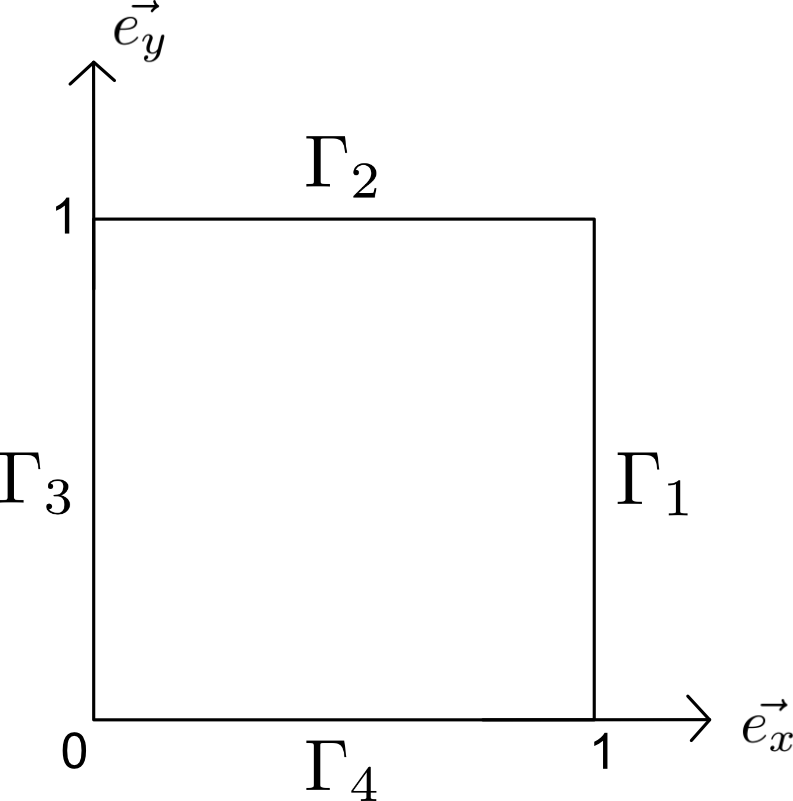
\includegraphics[height=7cm]{../Images/domaine1.png}
\end{center}

%%%%%%%%%%%%%%%%%%%%%%%%%%%%%%%%%
\subsection{Problème 1}
%%%%%%%%%%%%%%%%%%%%%%%%%%%%%%%%%


Le problème à résoudre est le suivant : 
\begin{align*}
    -\Delta u = f_\Omega
\end{align*}
La solution exacte est donnée pour $u=16xy(1-x)(1-y)$, ainsi on peut en déduire que :
\begin{align*}
    f_\Omega = 32\big( x(1-x) + y(1-y) \big)
\end{align*}
On impose une condition de Dirichlet homogène sur les 4 côtés, ainsi on a : 
\begin{align*}
    &\Gamma_D = \Gamma_1 \cup\Gamma_2 \cup\Gamma_3 \cup\Gamma_4 \\
    &\Gamma_N = \emptyset
\end{align*}
On doit également définir toutes les fonctions de la formulation variationelle comme suit : 
\begin{align*}
    &a_{\alpha\beta} = \delta_{\alpha\beta}\\
    &a_{00} = 0\\
    &b_N = 0\\
    &f_N = 0
\end{align*}

Après avoir exécuté le programme des éléments finis pour des maillages de plus en plus fins, on peut tracer une courbe qui nous montre l'erreur comparée à la solution exacte en fonction de la finesse du maillage.\\
Dans un premier temps on utilise des maillages constitués de triangles, on obtient la courbe suivante :

\begin{center}
    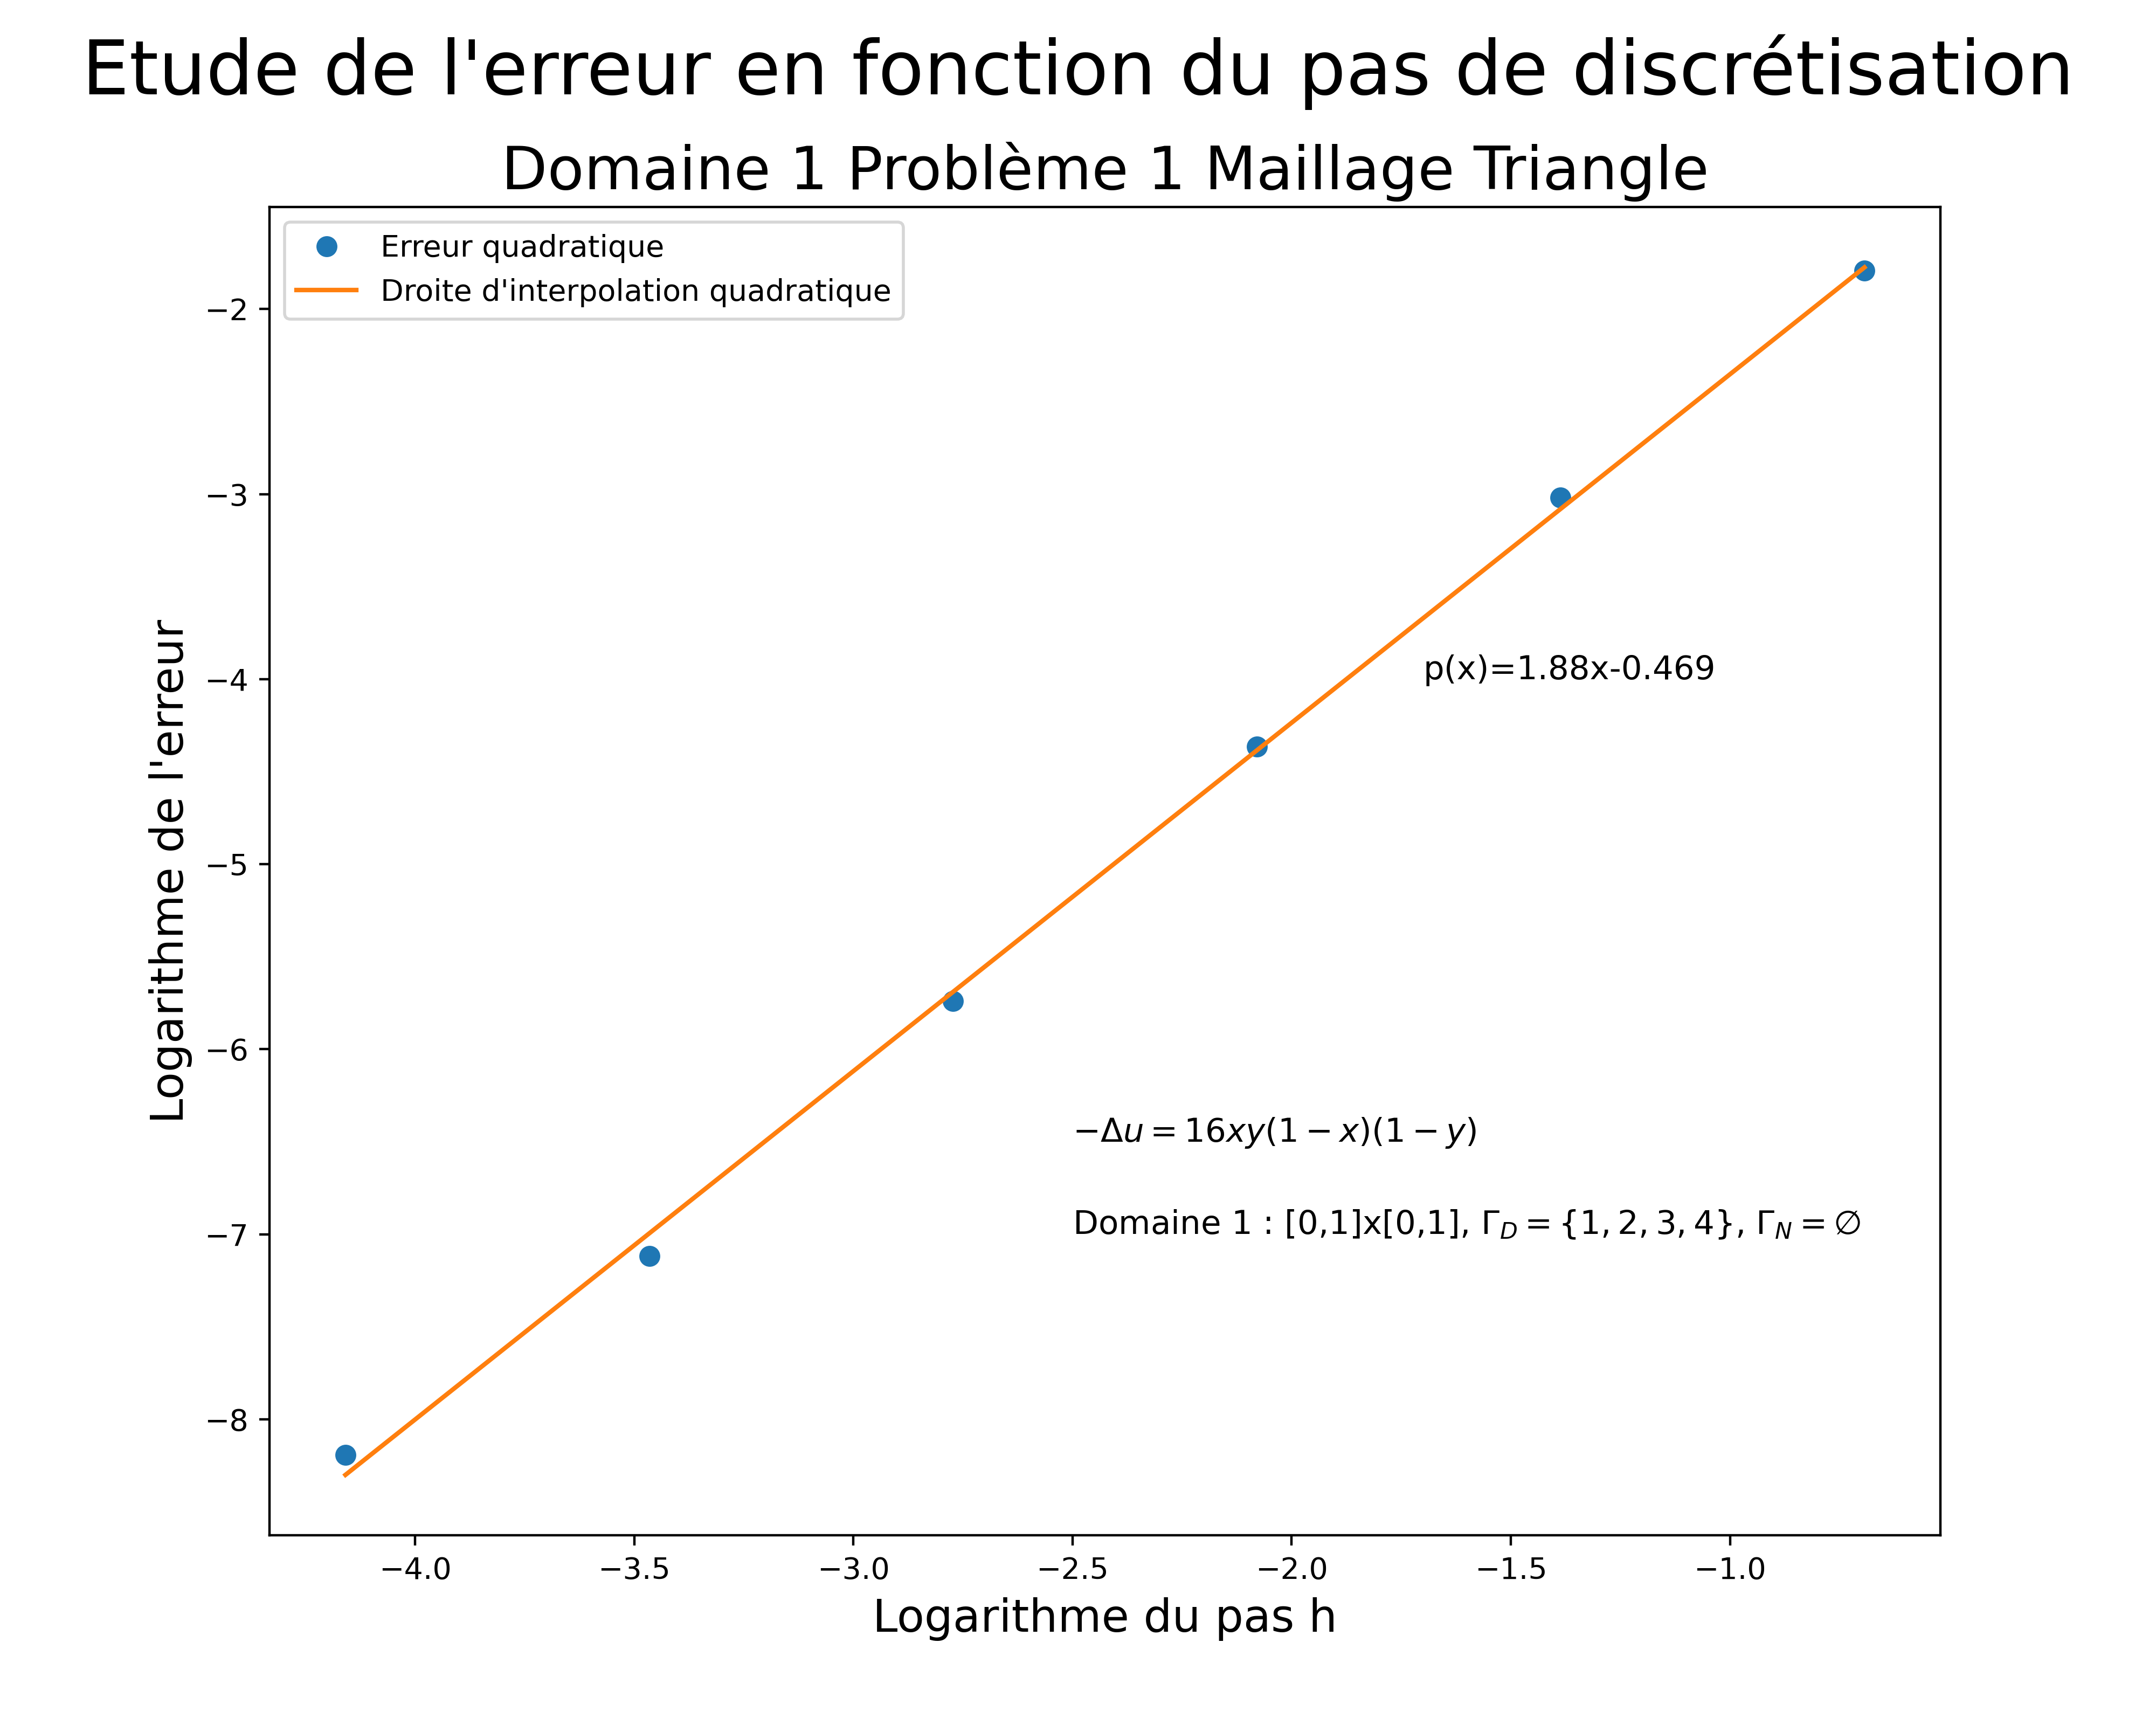
\includegraphics[height=10cm]{../Images/Courbes_Erreurs/D1P1T.png}
\end{center}

Dans un second temps, pour le même problème on utilise un maillage de quadrangle, on obtient alors la courbe suivante :
\begin{center}
    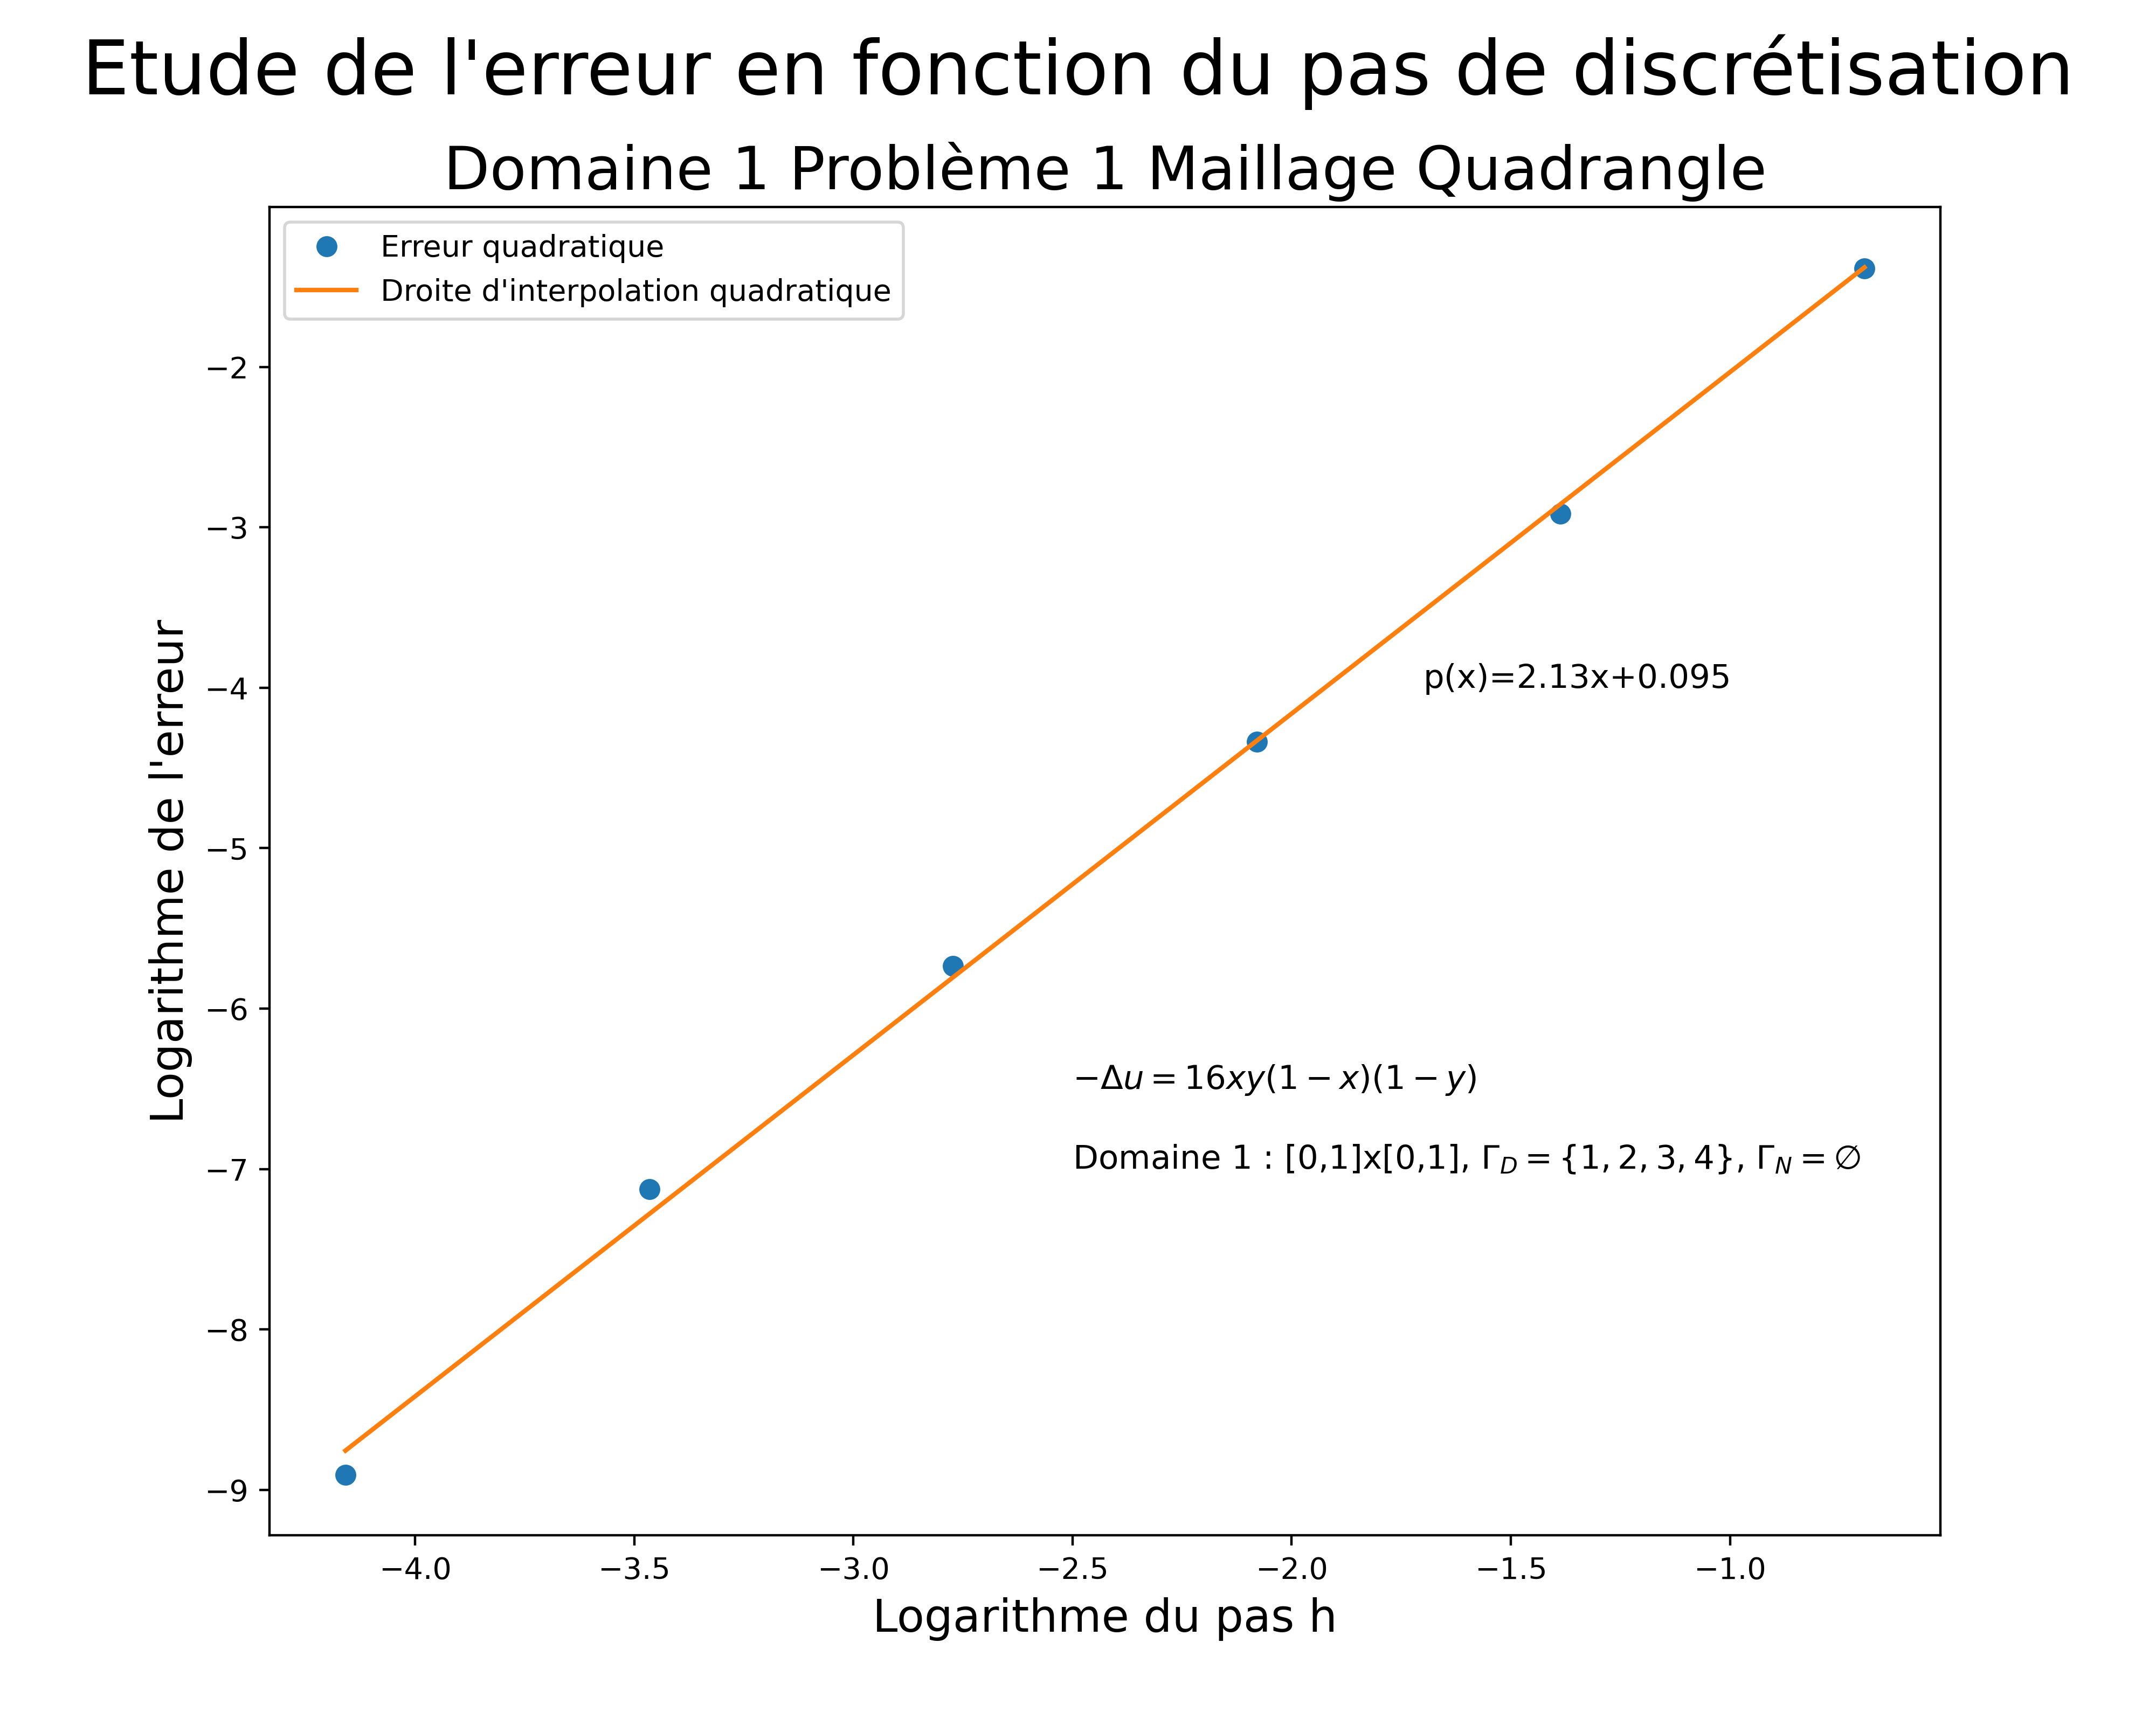
\includegraphics[height=10cm]{../Images/Courbes_Erreurs/D1P1Q.png}
\end{center}

On peut observer ici que l'interpolation des différents points nous donne un meilleur coefficient sur le maillage de type quadrangle (2.13) que de type triangle (1.88). 

On peut maintenant afficher la solution calculée en 3D pour visualiser la solution.
\begin{figure}[!h]
    \centering
    \begin{subfigure}{0.48\textwidth}
    	\centering
        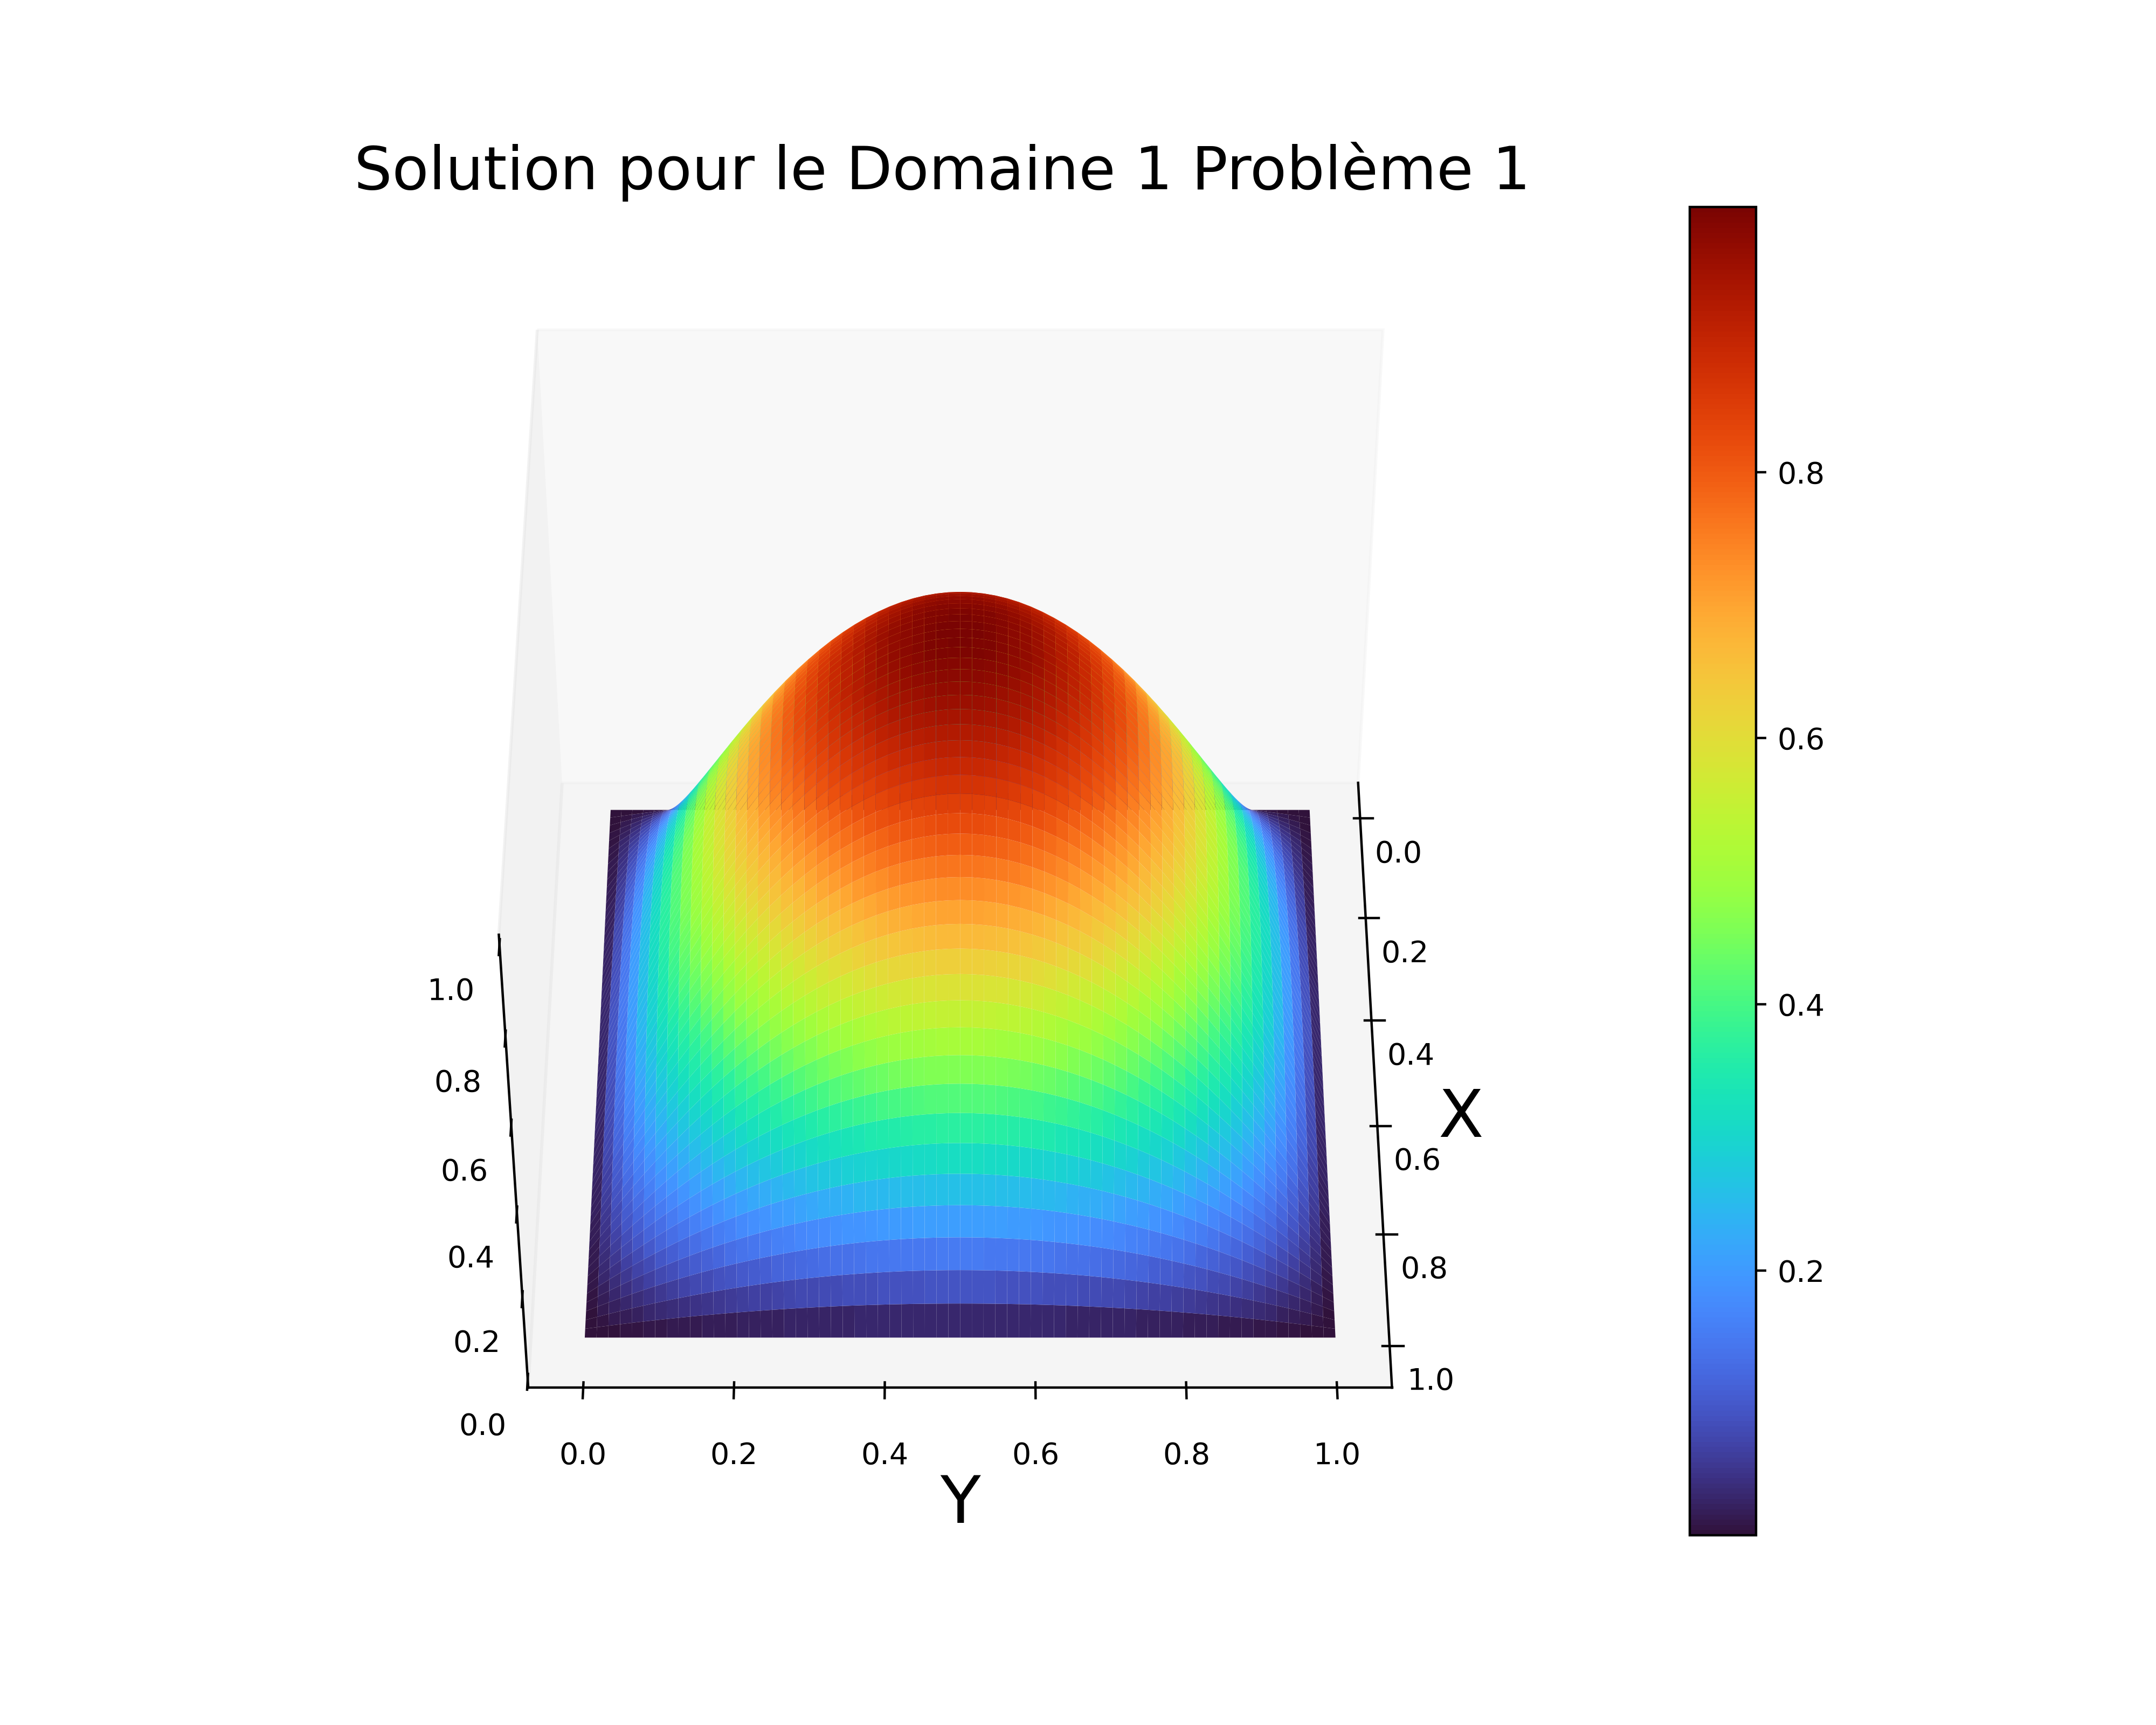
\includegraphics[height=9cm]{../Images/Figures_Calculees/sol3D11.png}
    \end{subfigure}
    \begin{subfigure}{0.48\textwidth}
    \centering
        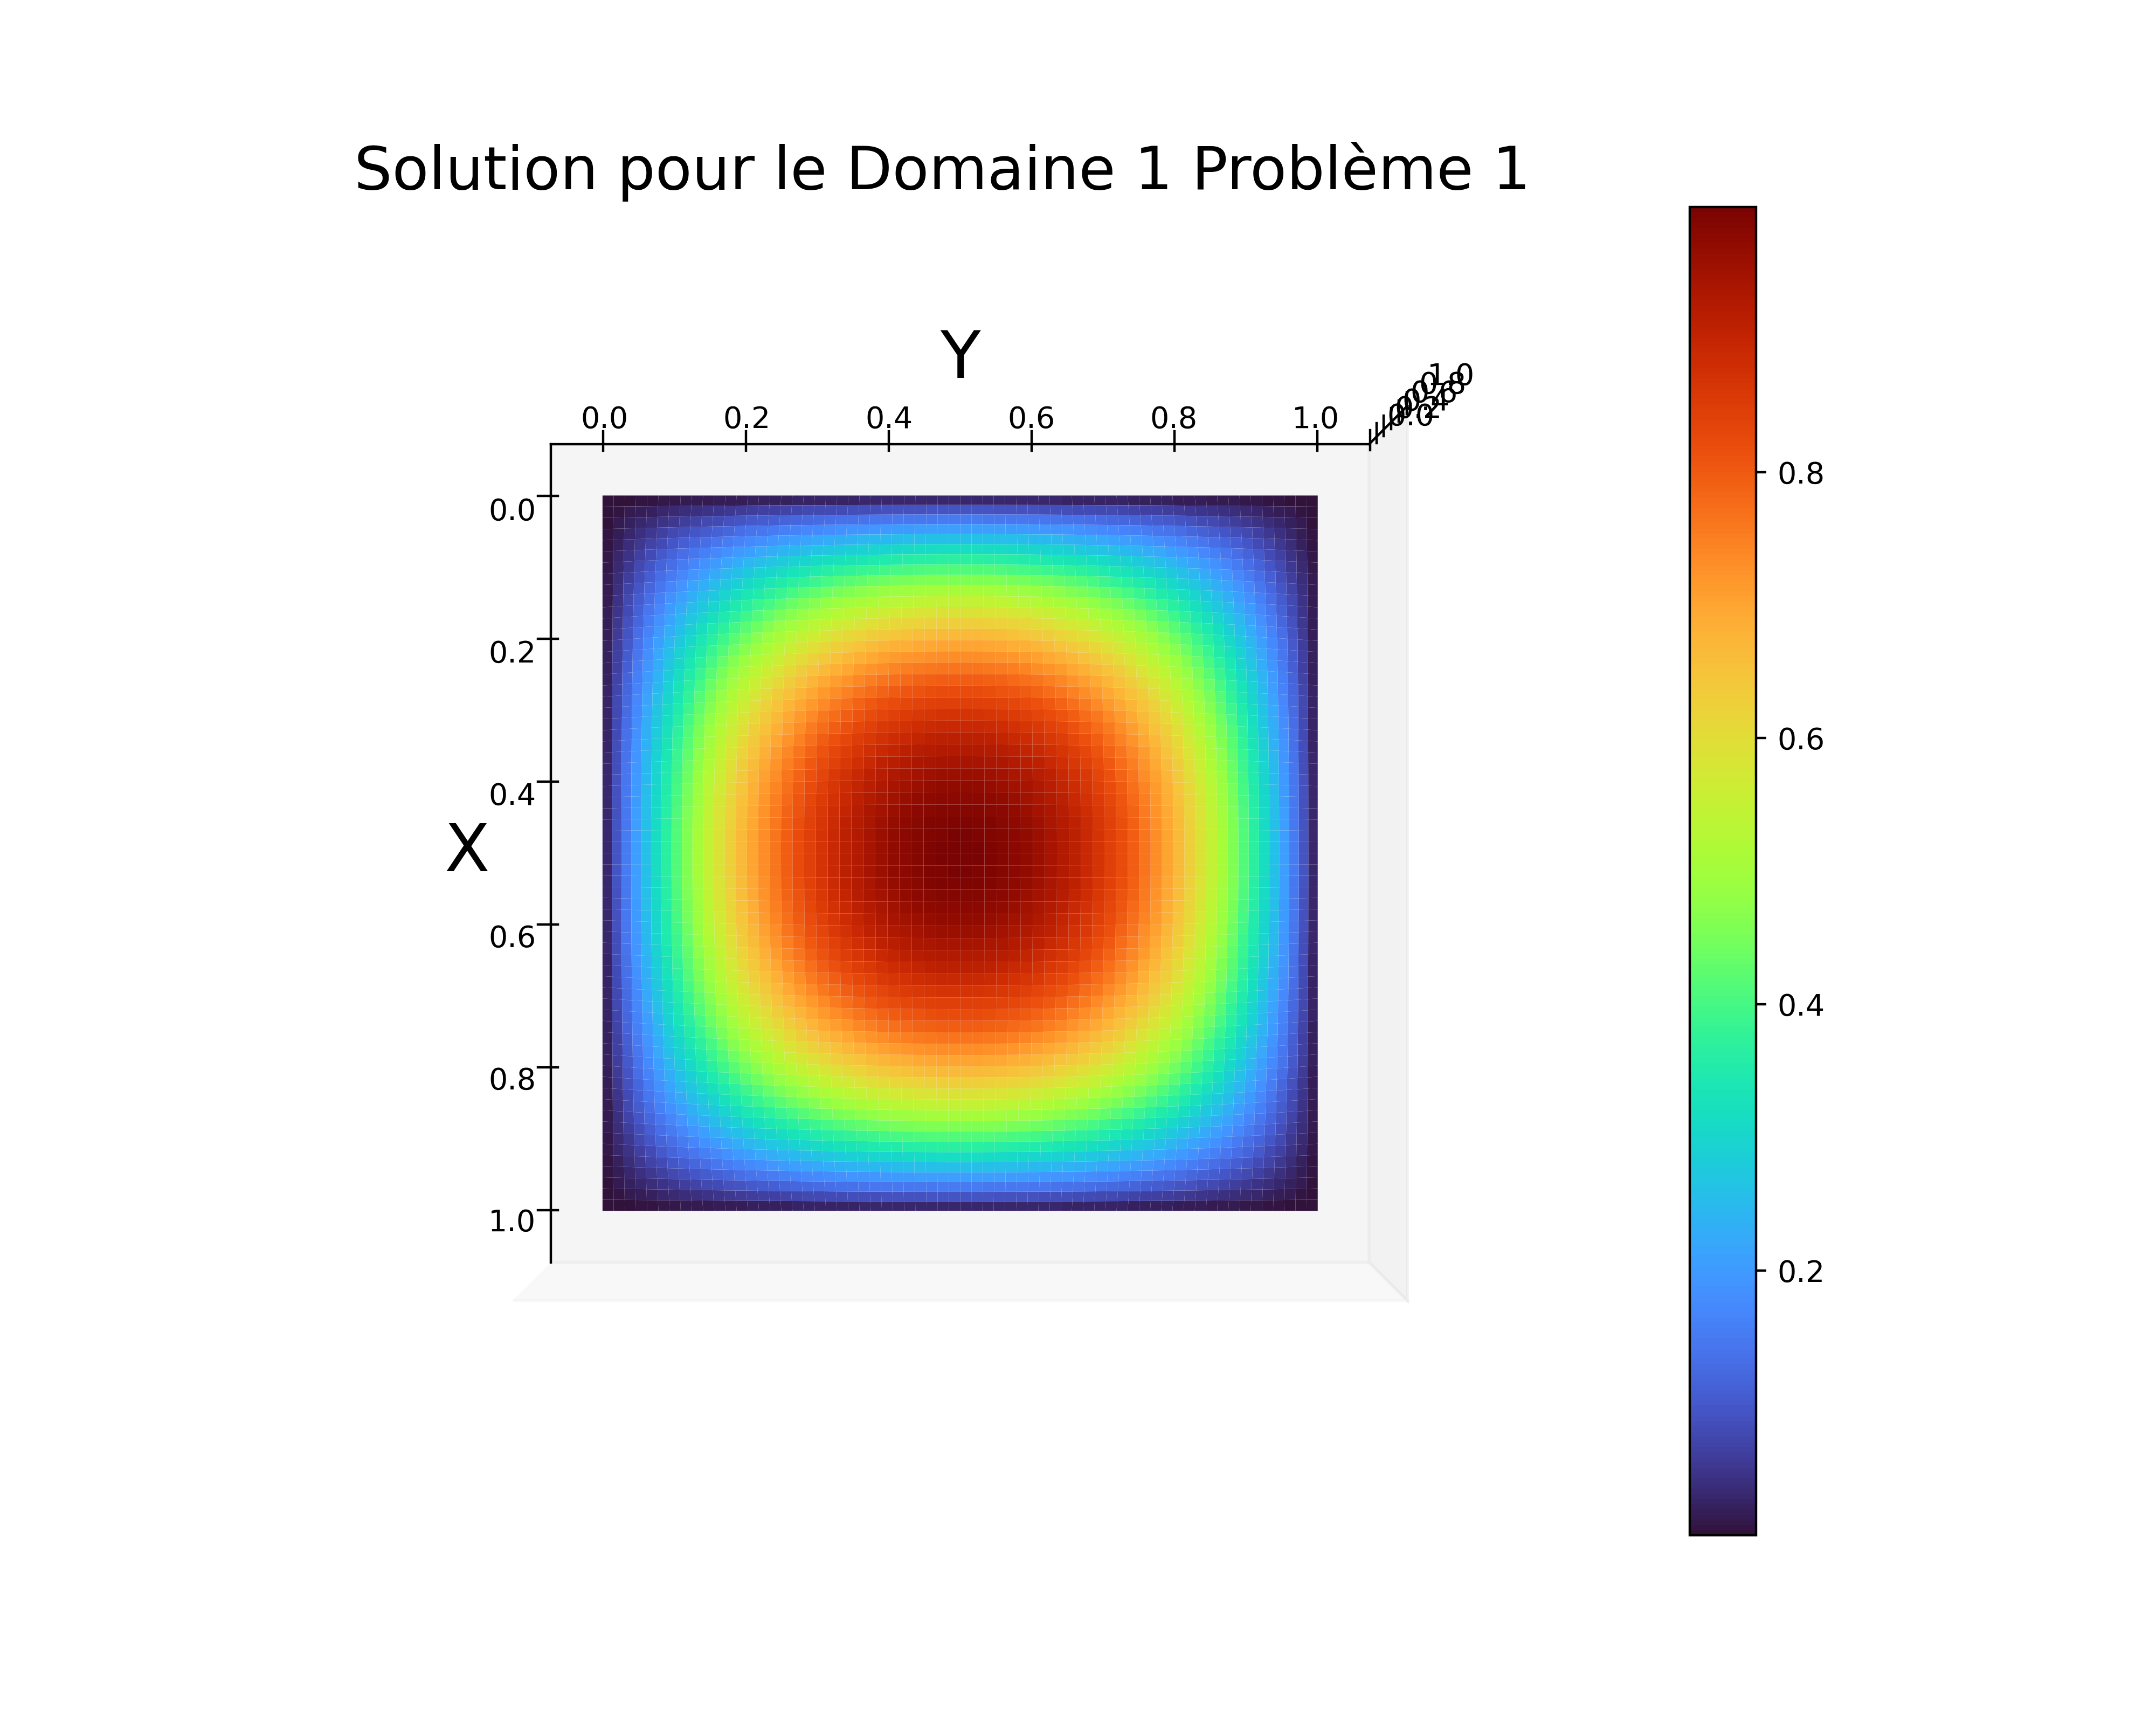
\includegraphics[height=9cm]{../Images/Figures_Calculees/sol3DVH11.png}
    \end{subfigure}
    \caption{Solution calculée vue sous différents angles Domaine 1 Problème 1 }
\end{figure}
%%%%%%%%%%%%%%%%%%%%%%%%%%%%%%%%%
\subsection{Problème 2}
%%%%%%%%%%%%%%%%%%%%%%%%%%%%%%%%%


Le problème à résoudre est le suivant : 
\begin{align*}
    -\Delta u = f_\Omega
\end{align*}
La solution exacte est donnée pour $u=\sin(\pi x)\sin(\pi y)$, ainsi on peut en déduire que :
\begin{align*}
    f_\Omega = 2\pi^2\sin(\pi x)\sin(\pi y)
\end{align*}
On impose également une condition de Dirichlet homogène sur les 4 côtés, ainsi on : 
\begin{align*}
    &\Gamma_D = \Gamma_1 \cup\Gamma_2 \cup\Gamma_3 \cup\Gamma_4\\
    &\Gamma_N = \emptyset
\end{align*}
Ici encore on doit également définir toutes les fonctions de la formulation variationelles qui sont les mêmes que dans le problème 1 : 
\begin{align*}
    &a_{\alpha\beta} = \delta_{\alpha\beta}\\
    &a_{00} = 0\\
    &b_N = 0\\
    &f_N = 0
\end{align*}
Après avoir exécuté le programme des éléments finis pour des maillages de plus en plus fin, on peut tracer une courbe qui nous montre l'erreur comparée à la solution exacte en fonction de la finesse du maillage.\\
Dans un premier temps on utilise des maillages constitués de triangles, on obtient la courbe suivante :

\begin{center}
    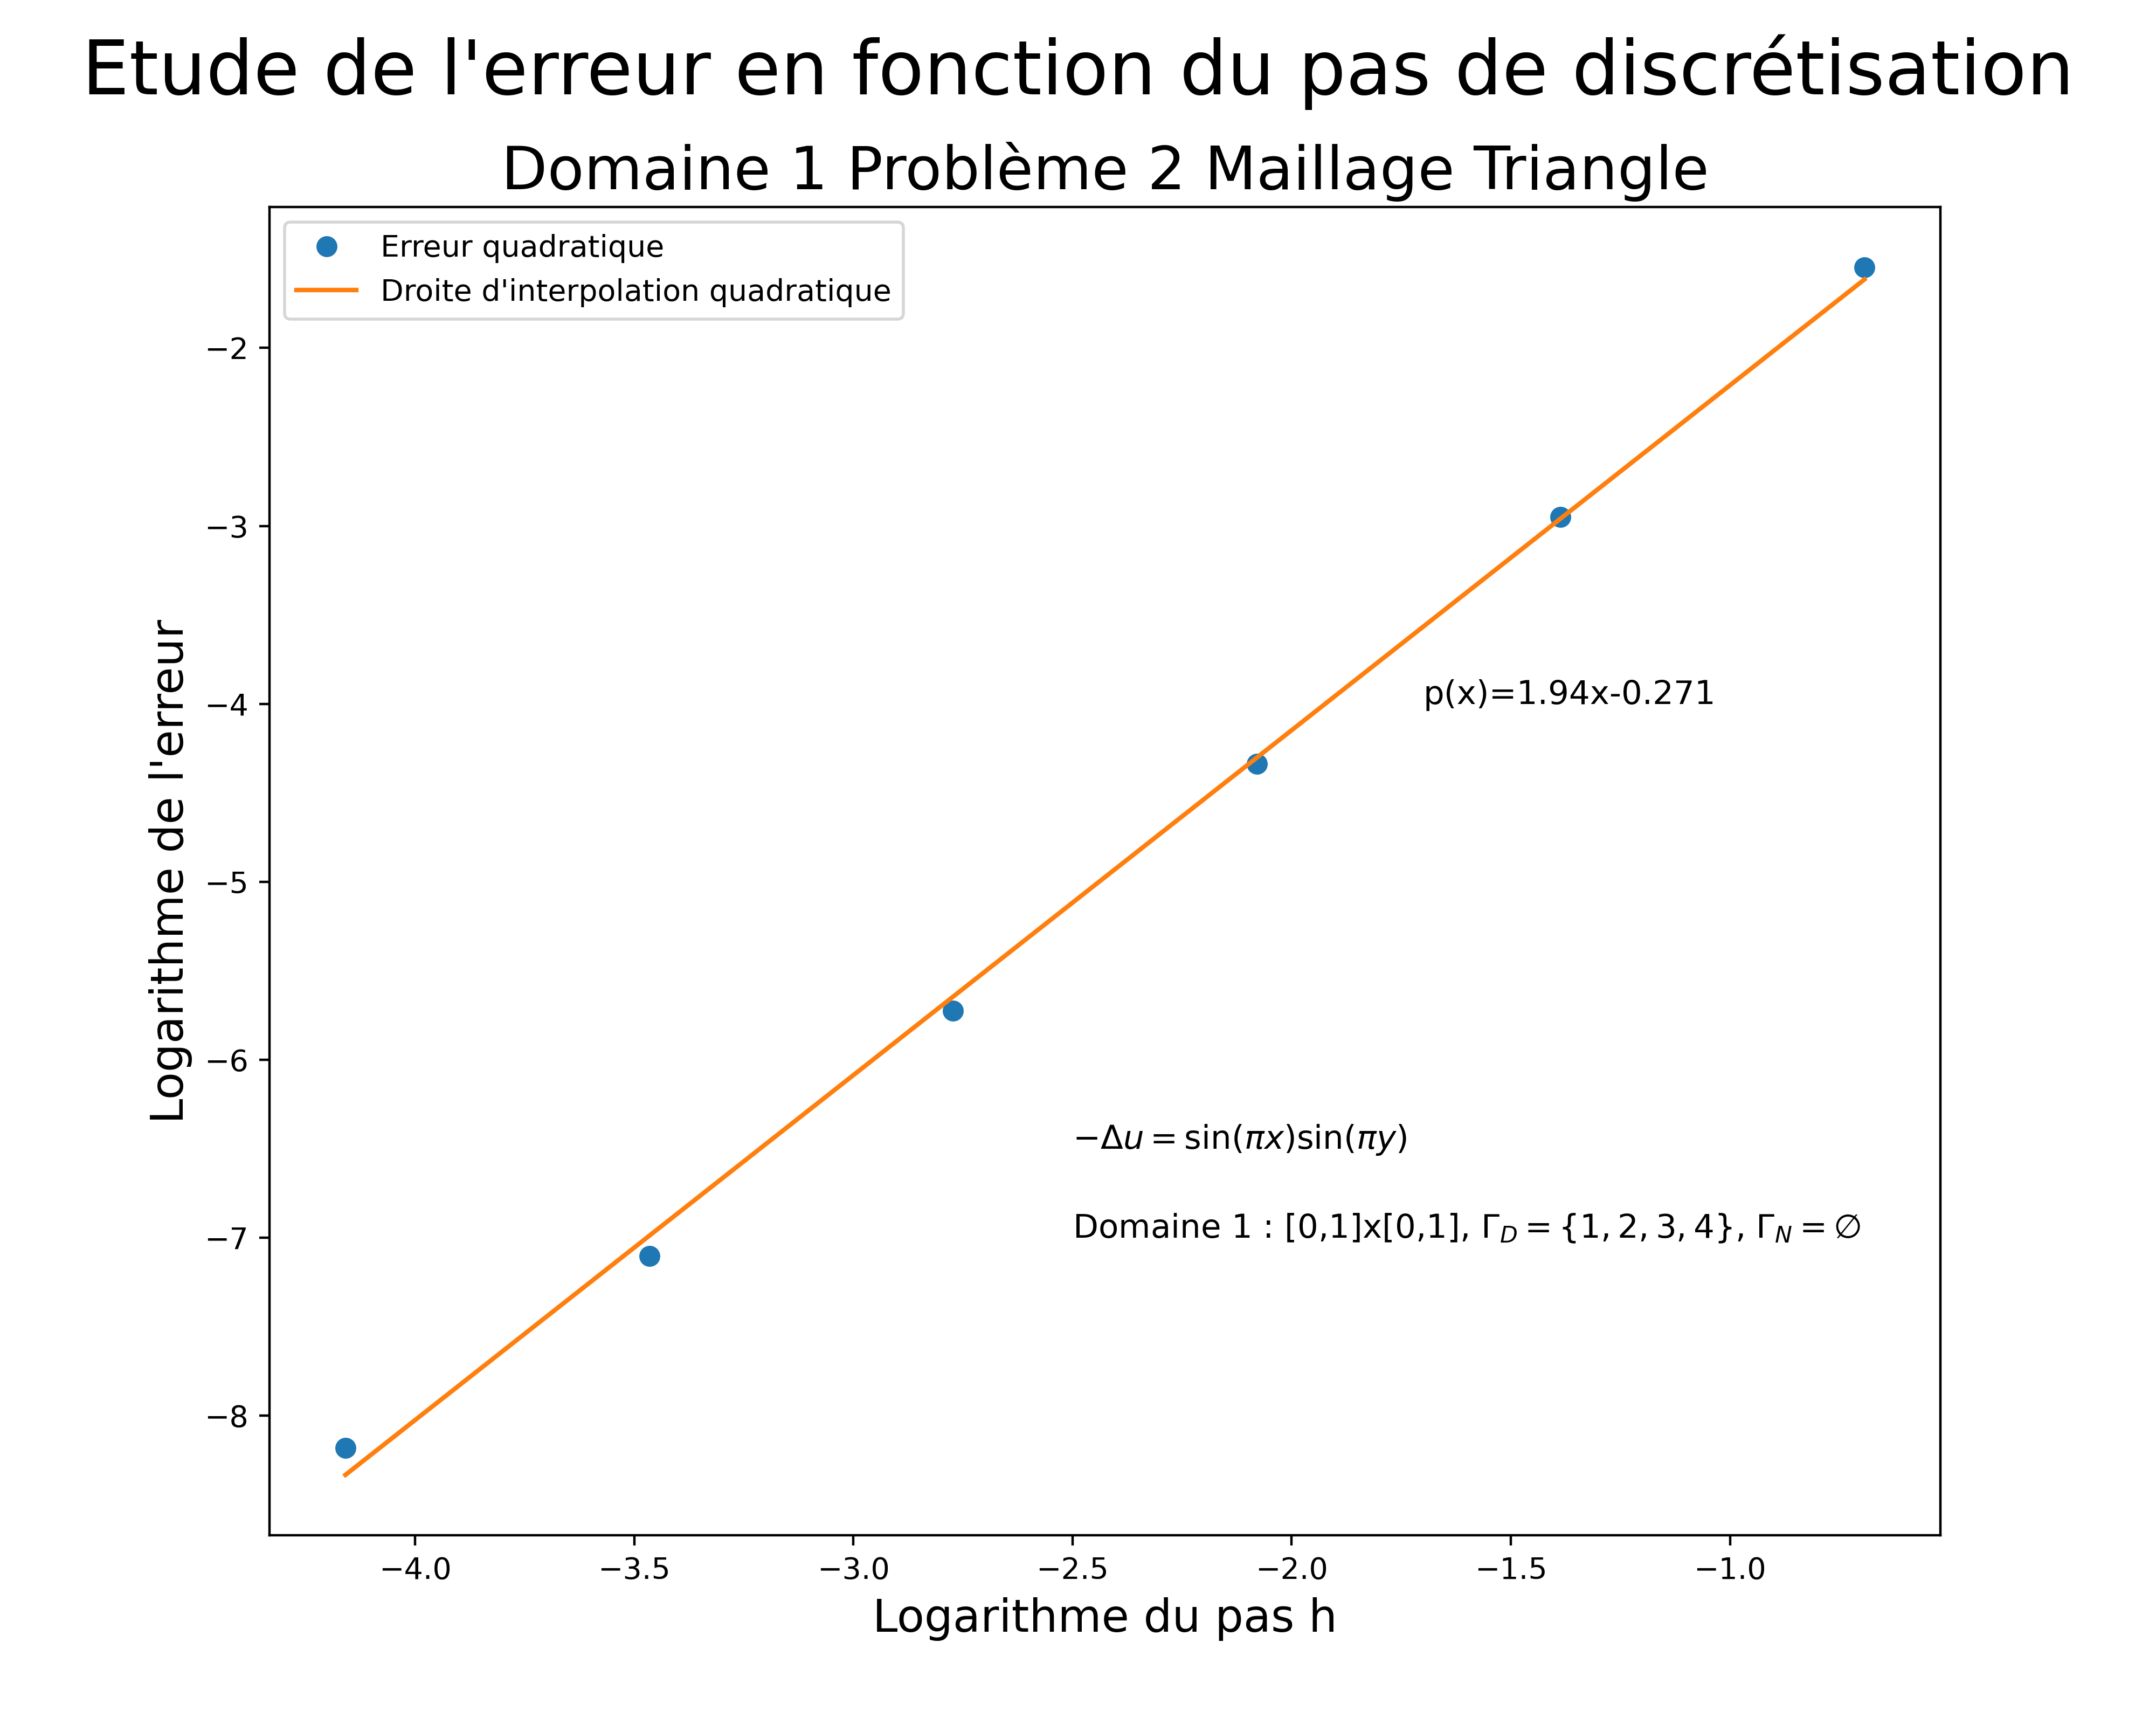
\includegraphics[height=9cm]{../Images/Courbes_Erreurs/D1P2T.png}
\end{center}

Dans un second temps, pour le même problème on utilise un maillage de quadrangle, on obtient alors la courbe suivante :
\begin{center}
    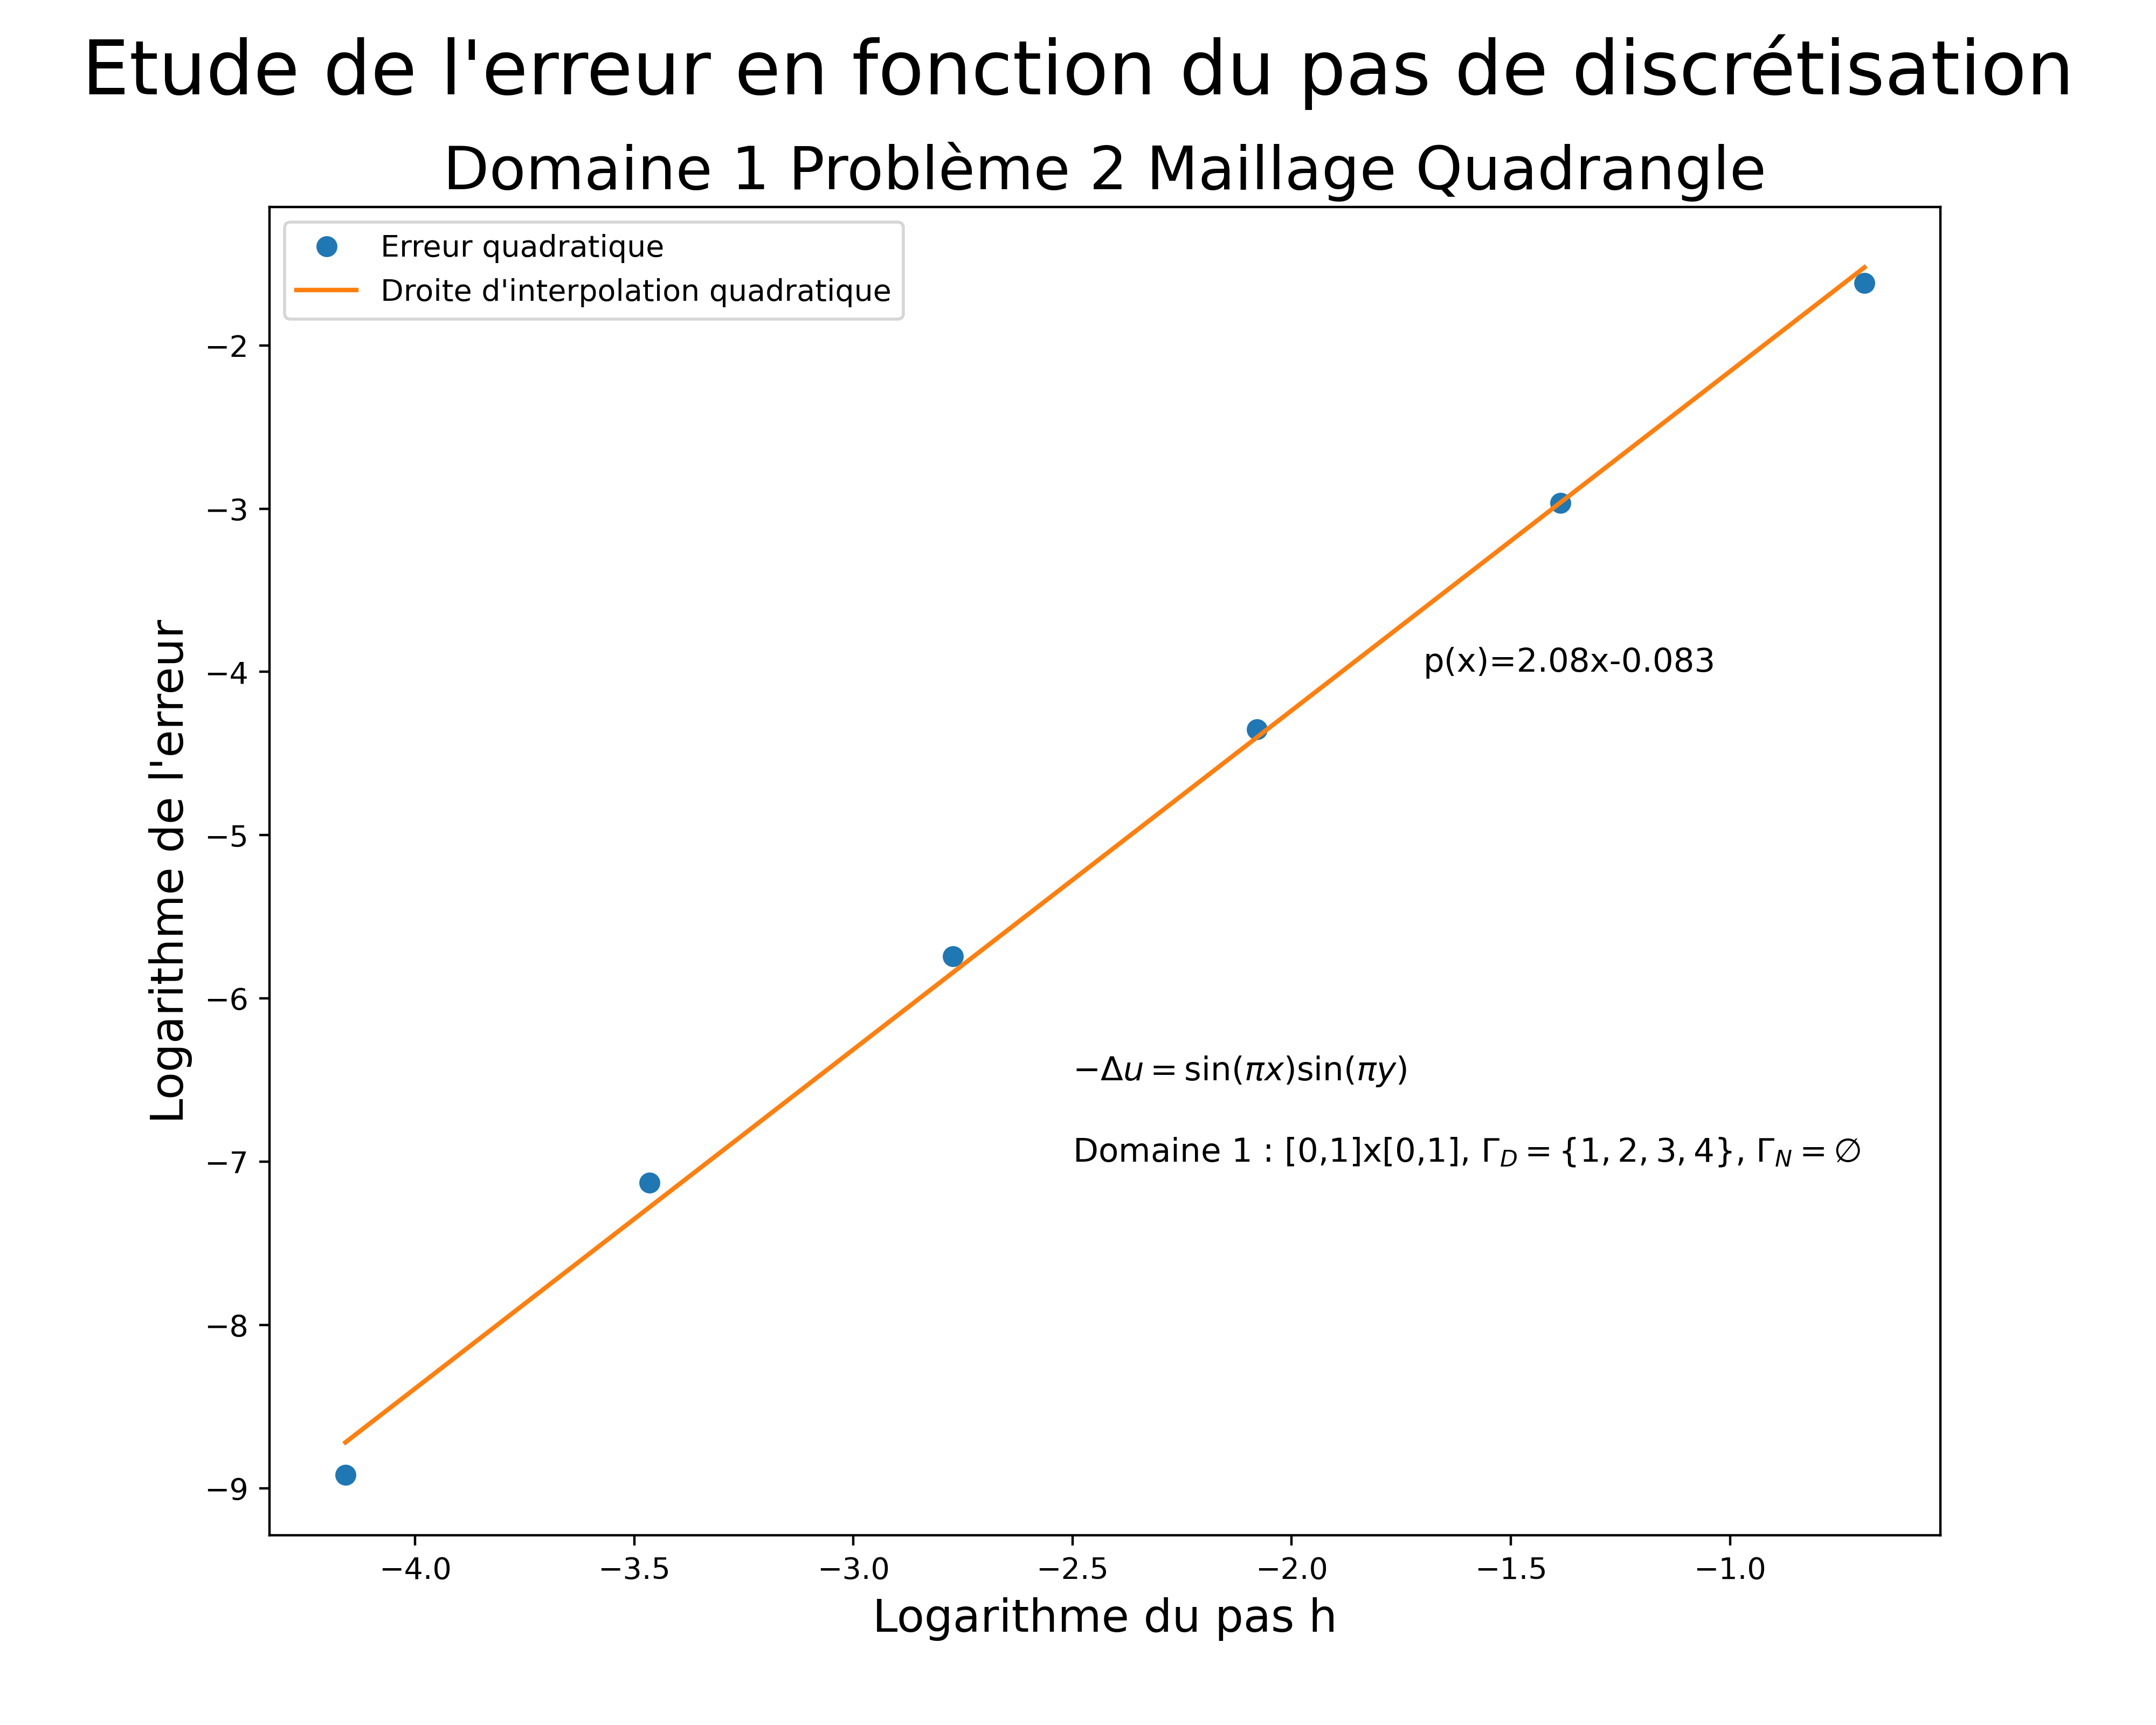
\includegraphics[height=9cm]{../Images/Courbes_Erreurs/D1P2Q.png}
\end{center}

On peut maintenant afficher la solution calculée en 3D pour visualiser la solution.
\begin{figure}[!h]
    \centering
    \begin{subfigure}{0.48\textwidth}
    	\centering
        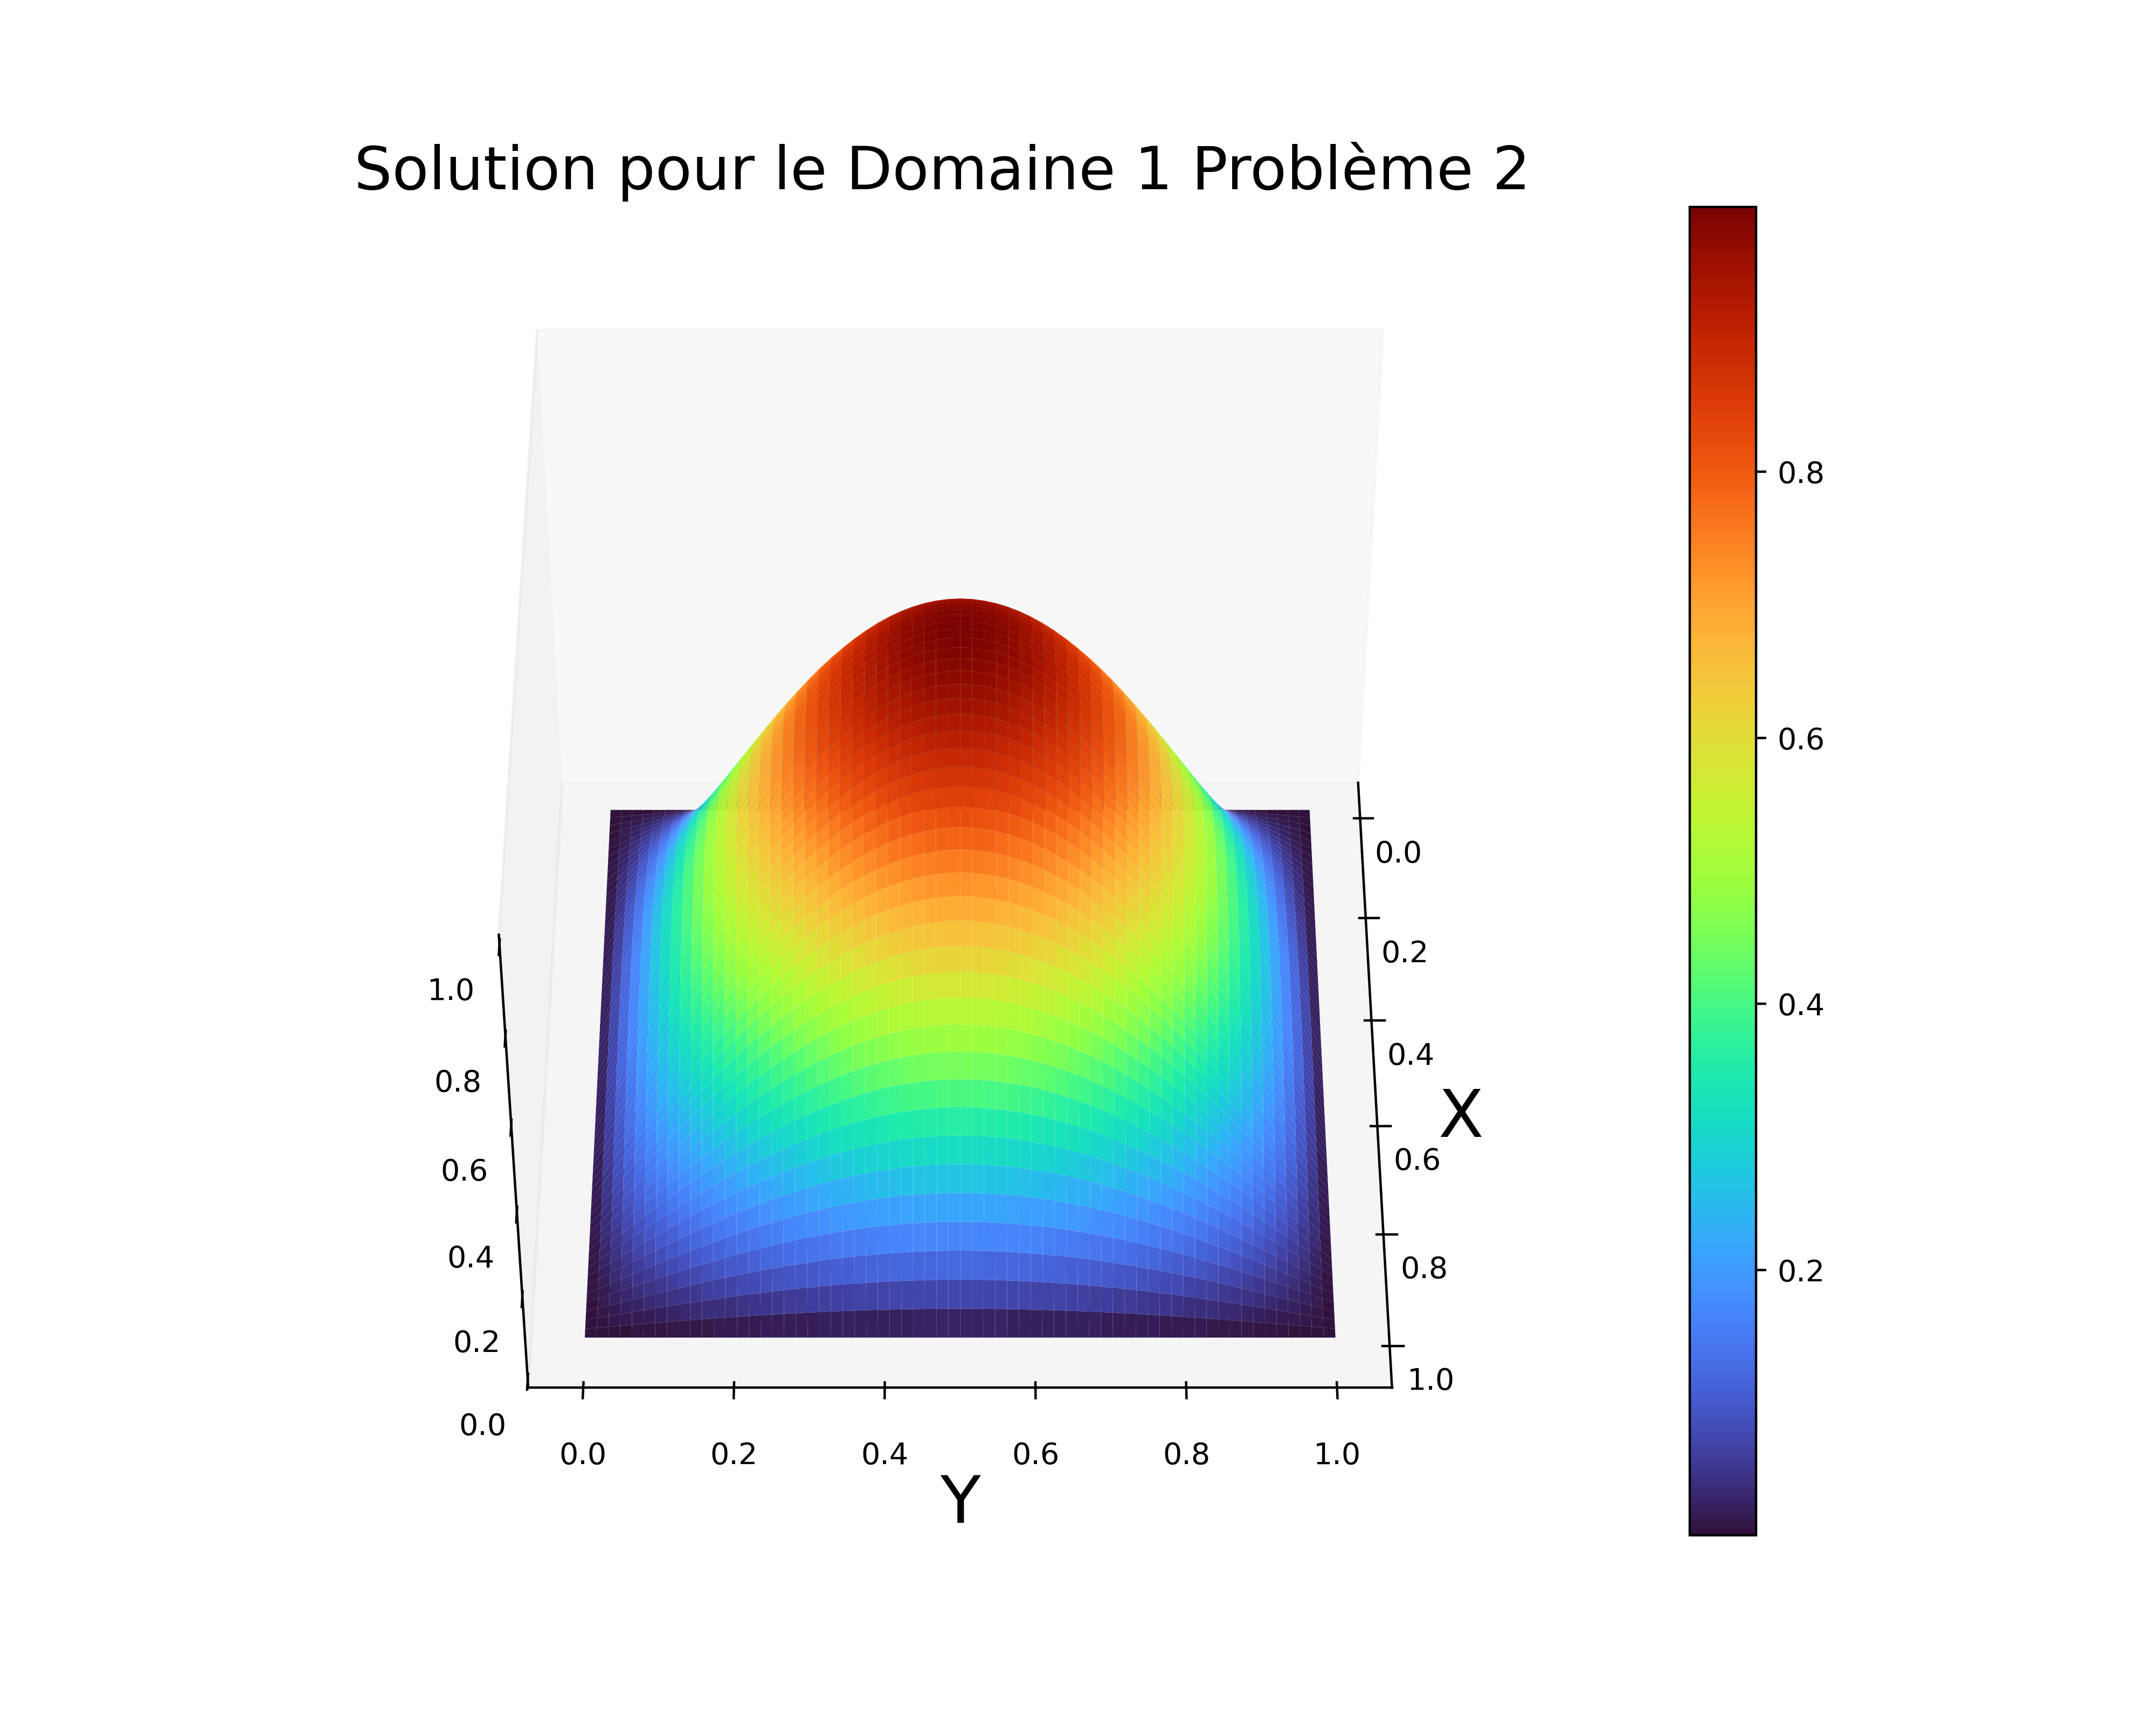
\includegraphics[height=9cm]{../Images/Figures_Calculees/sol3D12.png}
    \end{subfigure}
    \begin{subfigure}{0.48\textwidth}
    \centering
        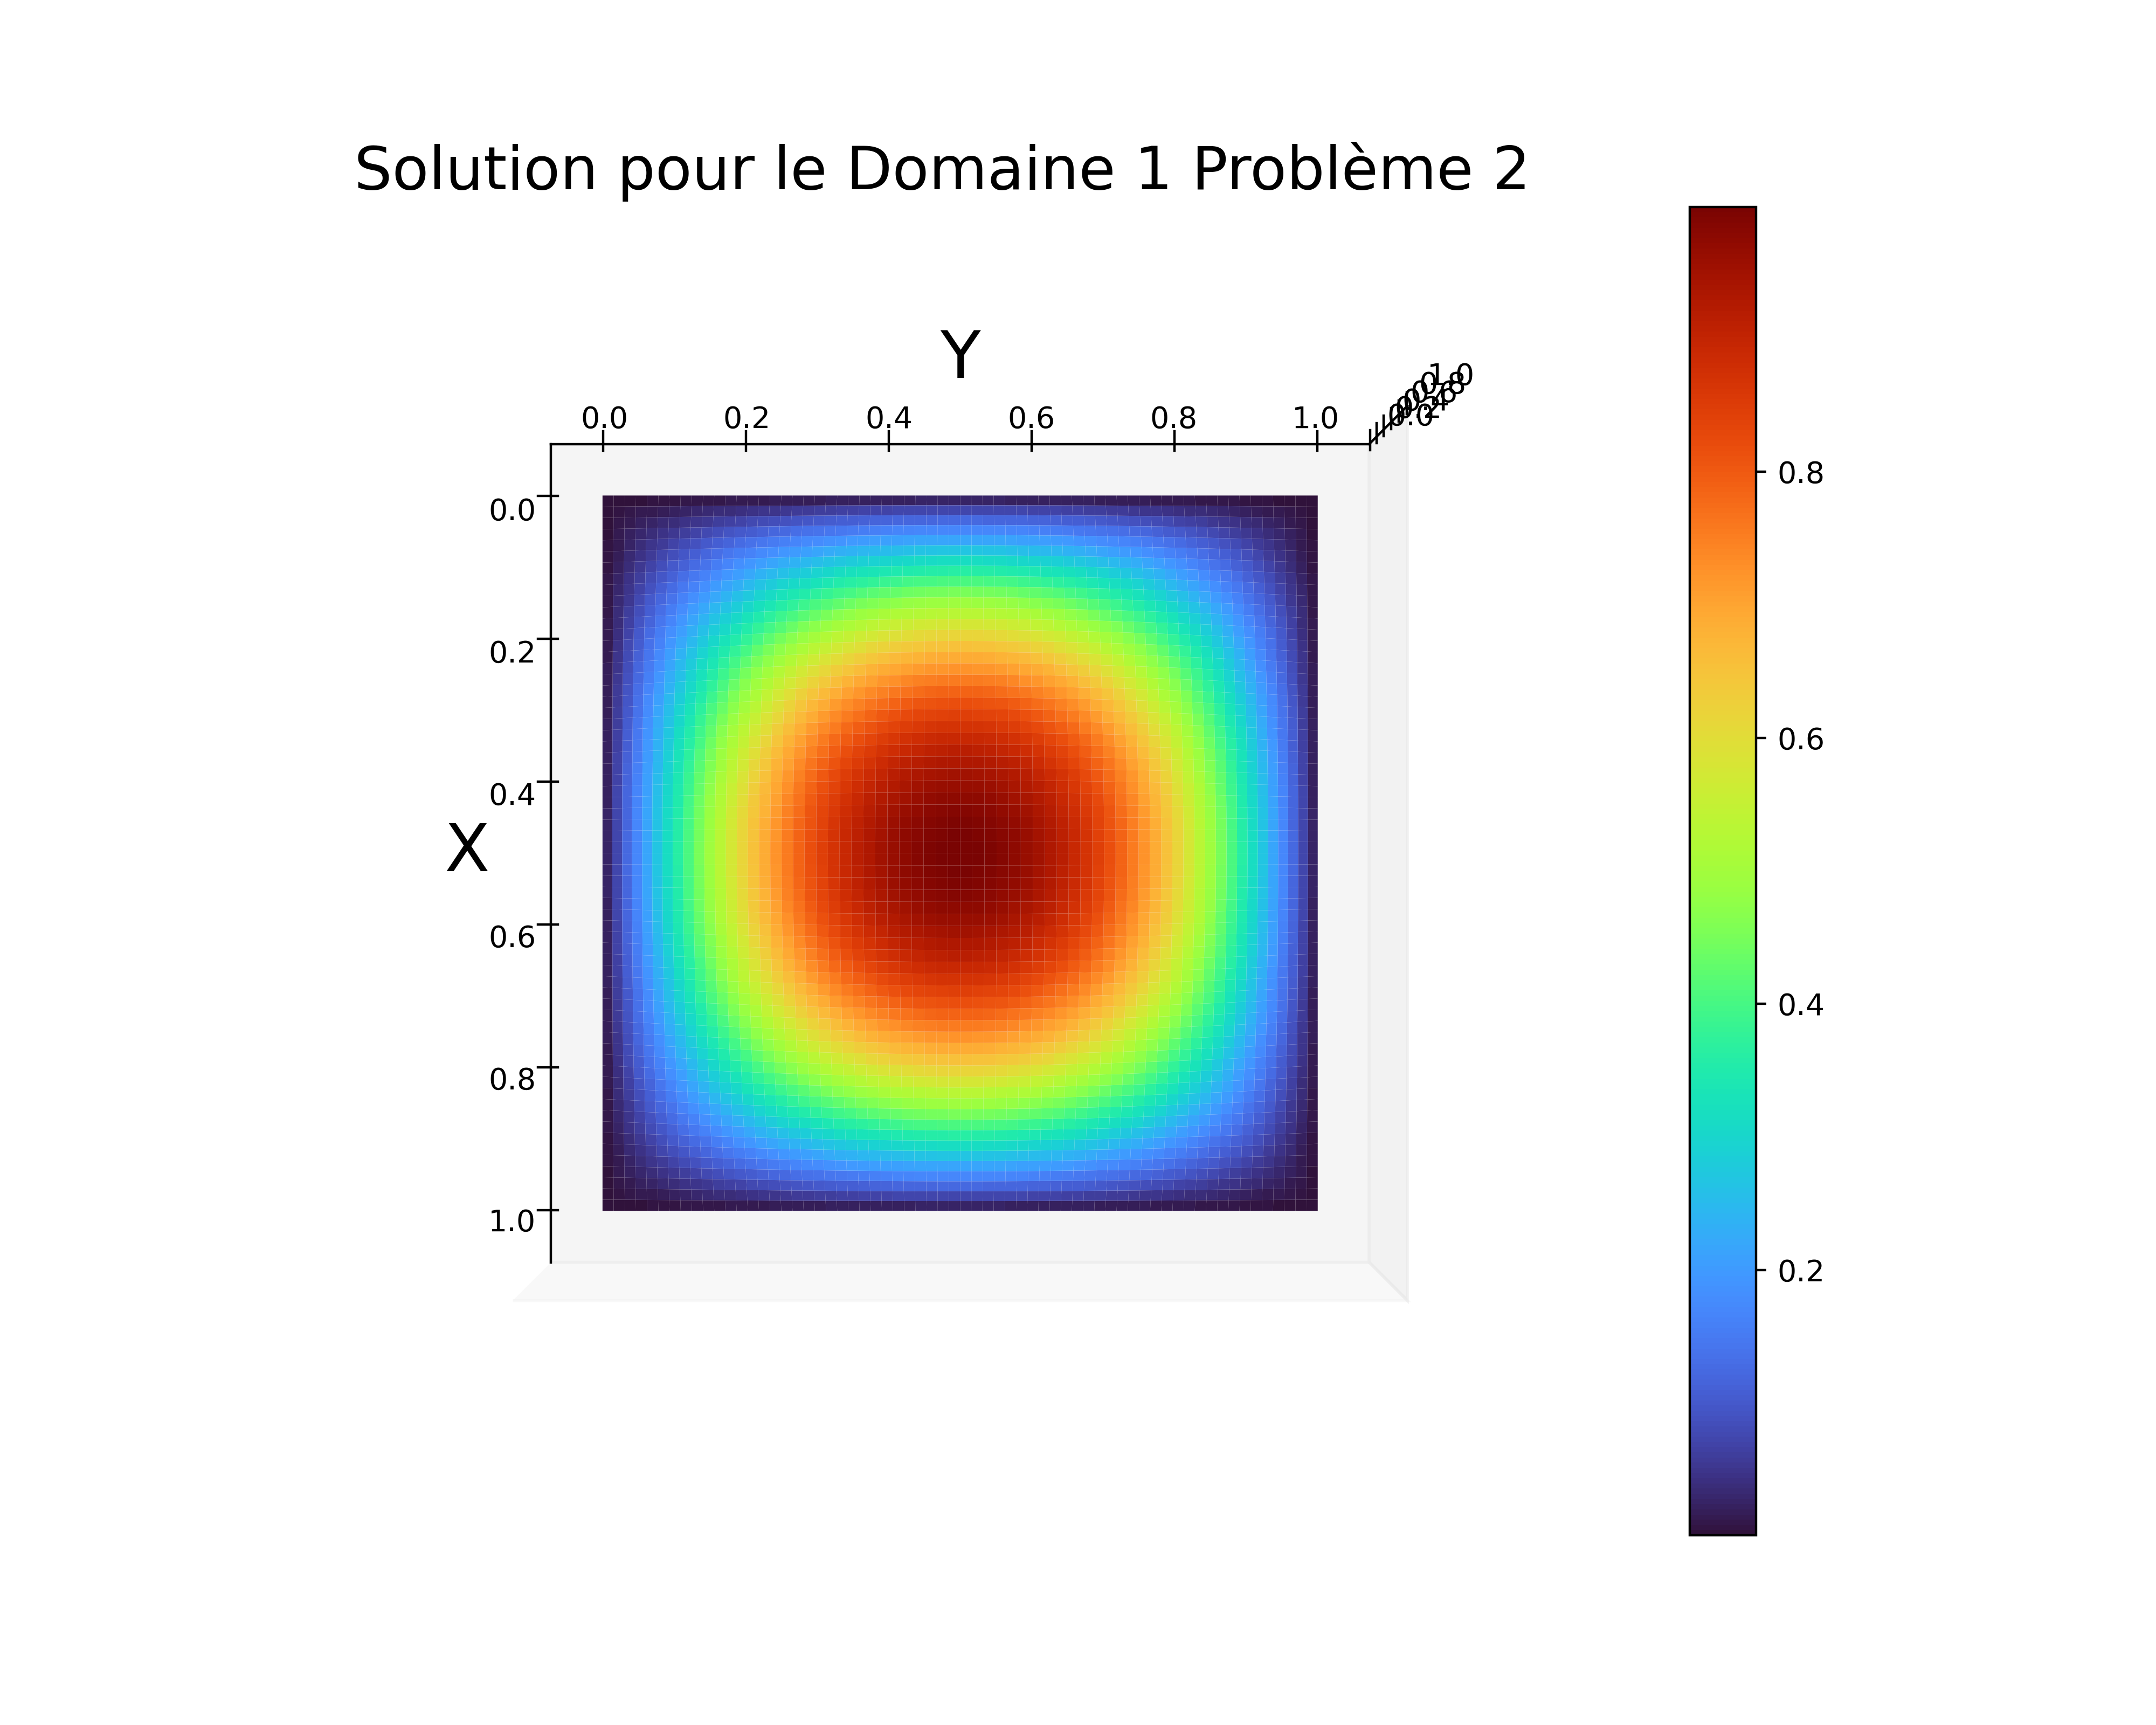
\includegraphics[height=9cm]{../Images/Figures_Calculees/sol3DVH12.png}
    \end{subfigure}
    \caption{Solution calculée vue sous différents angles Domaine 1 Problème 2 }
\end{figure}
\newpage
%%%%%%%%%%%%%%%%%%%%%%%%%%%%%%%%%
\subsection{Problème 3}
%%%%%%%%%%%%%%%%%%%%%%%%%%%%%%%%%


Le problème à résoudre est le suivant : 

\begin{align}
    \left\{
    \begin{array}{ll}
        -\Delta u + u = f_\Omega \\
        \Gamma_D = \emptyset\\
        \Gamma_N = \Gamma_1 \cup\Gamma_2 \cup\Gamma_3 \cup\Gamma_4
    \end{array}
    \right.
\end{align}
La solution exacte est donnée pour $u=\cos(\pi x)\cos(\pi y)$, ainsi on peut en déduire que :
\begin{align*}
    &\Delta u(x,y) = -2\pi^2\cos(\pi x)\cos(\pi y)\\
    \Rightarrow &f_\Omega =(1+2\pi^2)\cos(\pi x)\cos(\pi y)
\end{align*}
On impose ici une condition de Neumann homogène sur les 4 côtés, ainsi on a : 
\begin{align*}
    &\Gamma_D = \emptyset\\
    &\Gamma_N = \Gamma_1 \cup\Gamma_2 \cup\Gamma_3 \cup\Gamma_4
\end{align*}
On doit donc également déduire $f_N$.\\
On a $\Vec{n}_{|\Gamma_1} = \Vec{e_x}$, $\Vec{n}_{|\Gamma_2} = \Vec{e_y}$, $\Vec{n}_{|\Gamma_3} = -\Vec{e_x}$ et $\Vec{n}_{|\Gamma_4} = -\Vec{e_y}$ et également :
\\$\nabla u(x,y) = \Big(-\pi \sin(\pi x)\cos(\pi y), -\pi \cos(\pi x)\sin(\pi y) \Big)^T$ on peut donc en déduire que :
\begin{align*}
    &\frac{\partial u}{\partial \Vec{n}_{|\Gamma_1}} = \nabla u \cdot \Vec{e_x} = -\pi \sin(\pi x)\cos(\pi y)\\
    &\frac{\partial u}{\partial \Vec{n}_{|\Gamma_2}} = \nabla u \cdot \Vec{e_y} = -\pi \cos(\pi x)\sin(\pi y)\\
    &\frac{\partial u}{\partial \Vec{n}_{|\Gamma_3}} = \nabla u \cdot (-\Vec{e_x}) = \pi \sin(\pi x)\cos(\pi y)\\
    &\frac{\partial u}{\partial \Vec{n}_{|\Gamma_4}} = \nabla u \cdot (-\Vec{e_y}) = \pi \cos(\pi x)\sin(\pi y)
\end{align*}

Ainsi on peut définir la fonction $f_N$ comme suit :

\begin{align*}
    f_N = \left\{
    \begin{array}{ll}
        -\pi \sin(\pi x)\cos(\pi y)  \quad &\text{ sur $\Gamma_1$}\\
        -\pi \cos(\pi x)\sin(\pi y)\quad &\text{ sur $\Gamma_2$}\\
        \pi \sin(\pi x)\cos(\pi y)\quad &\text{ sur $\Gamma_3$}\\
        \pi \cos(\pi x)\sin(\pi y)\quad &\text{ sur $\Gamma_4$}\\
    \end{array}
    \right.
\end{align*}
Il faut alors faire attention à ce que les conditions aux bords soit placées sur les bonnes arêtes, il faut donc corréler la définition de la fonction $f_N$ avec le maillage que l'on prend en entrée.

On doit également définir toutes les fonctions de la formulation variationelles comme suit : 
\begin{align*}
    &a_{\alpha\beta} = \delta_{\alpha\beta}\\
    &a_{00} = 1\\
    &b_N = 0
\end{align*}

Après avoir exécuté le programme des éléments finis pour des maillages de plus en plus fin, on peut tracer une courbe qui nous montre l'erreur comparée à la solution exacte en fonction de la finesse du maillage.\\
Dans un premier temps on utilise des maillages constitués de triangles, on obtient la courbe suivante :

\begin{center}
    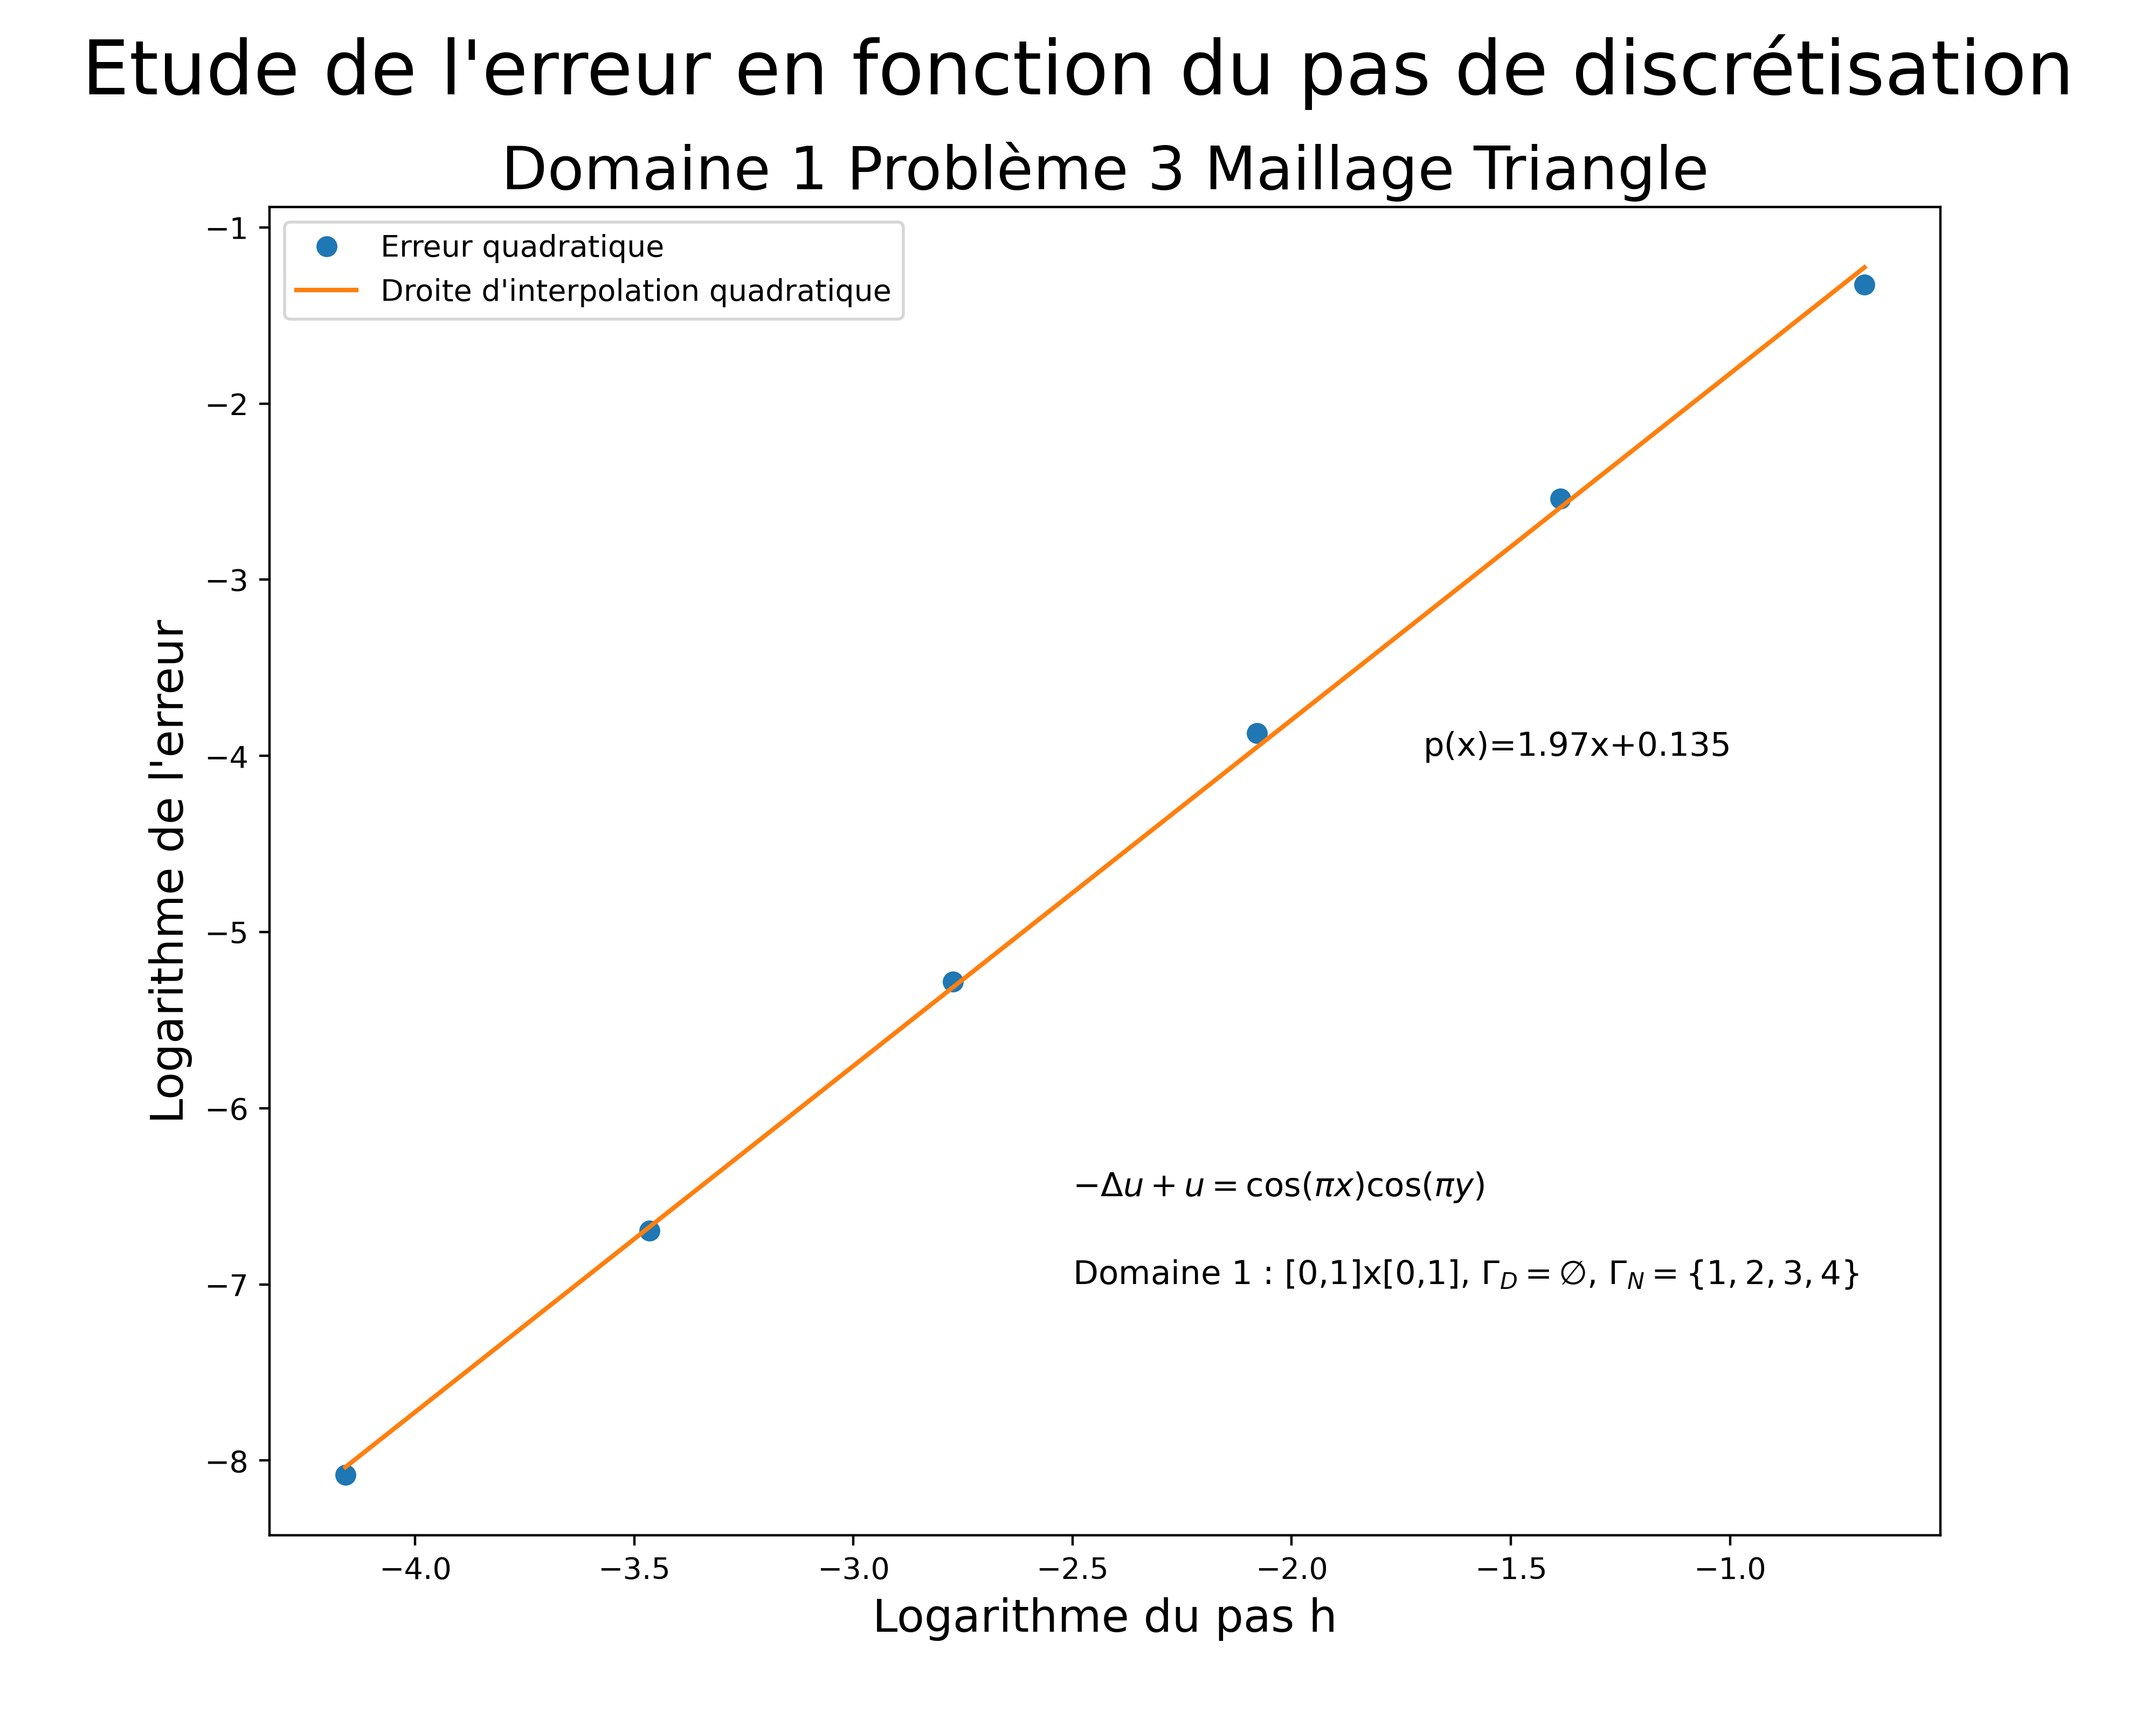
\includegraphics[height=9cm]{../Images/Courbes_Erreurs/D1P3T.png}
\end{center}

Dans un second temps, pour le même problème on utilise un maillage de quadrangle, on obtient alors la courbe suivante :
\begin{center}
    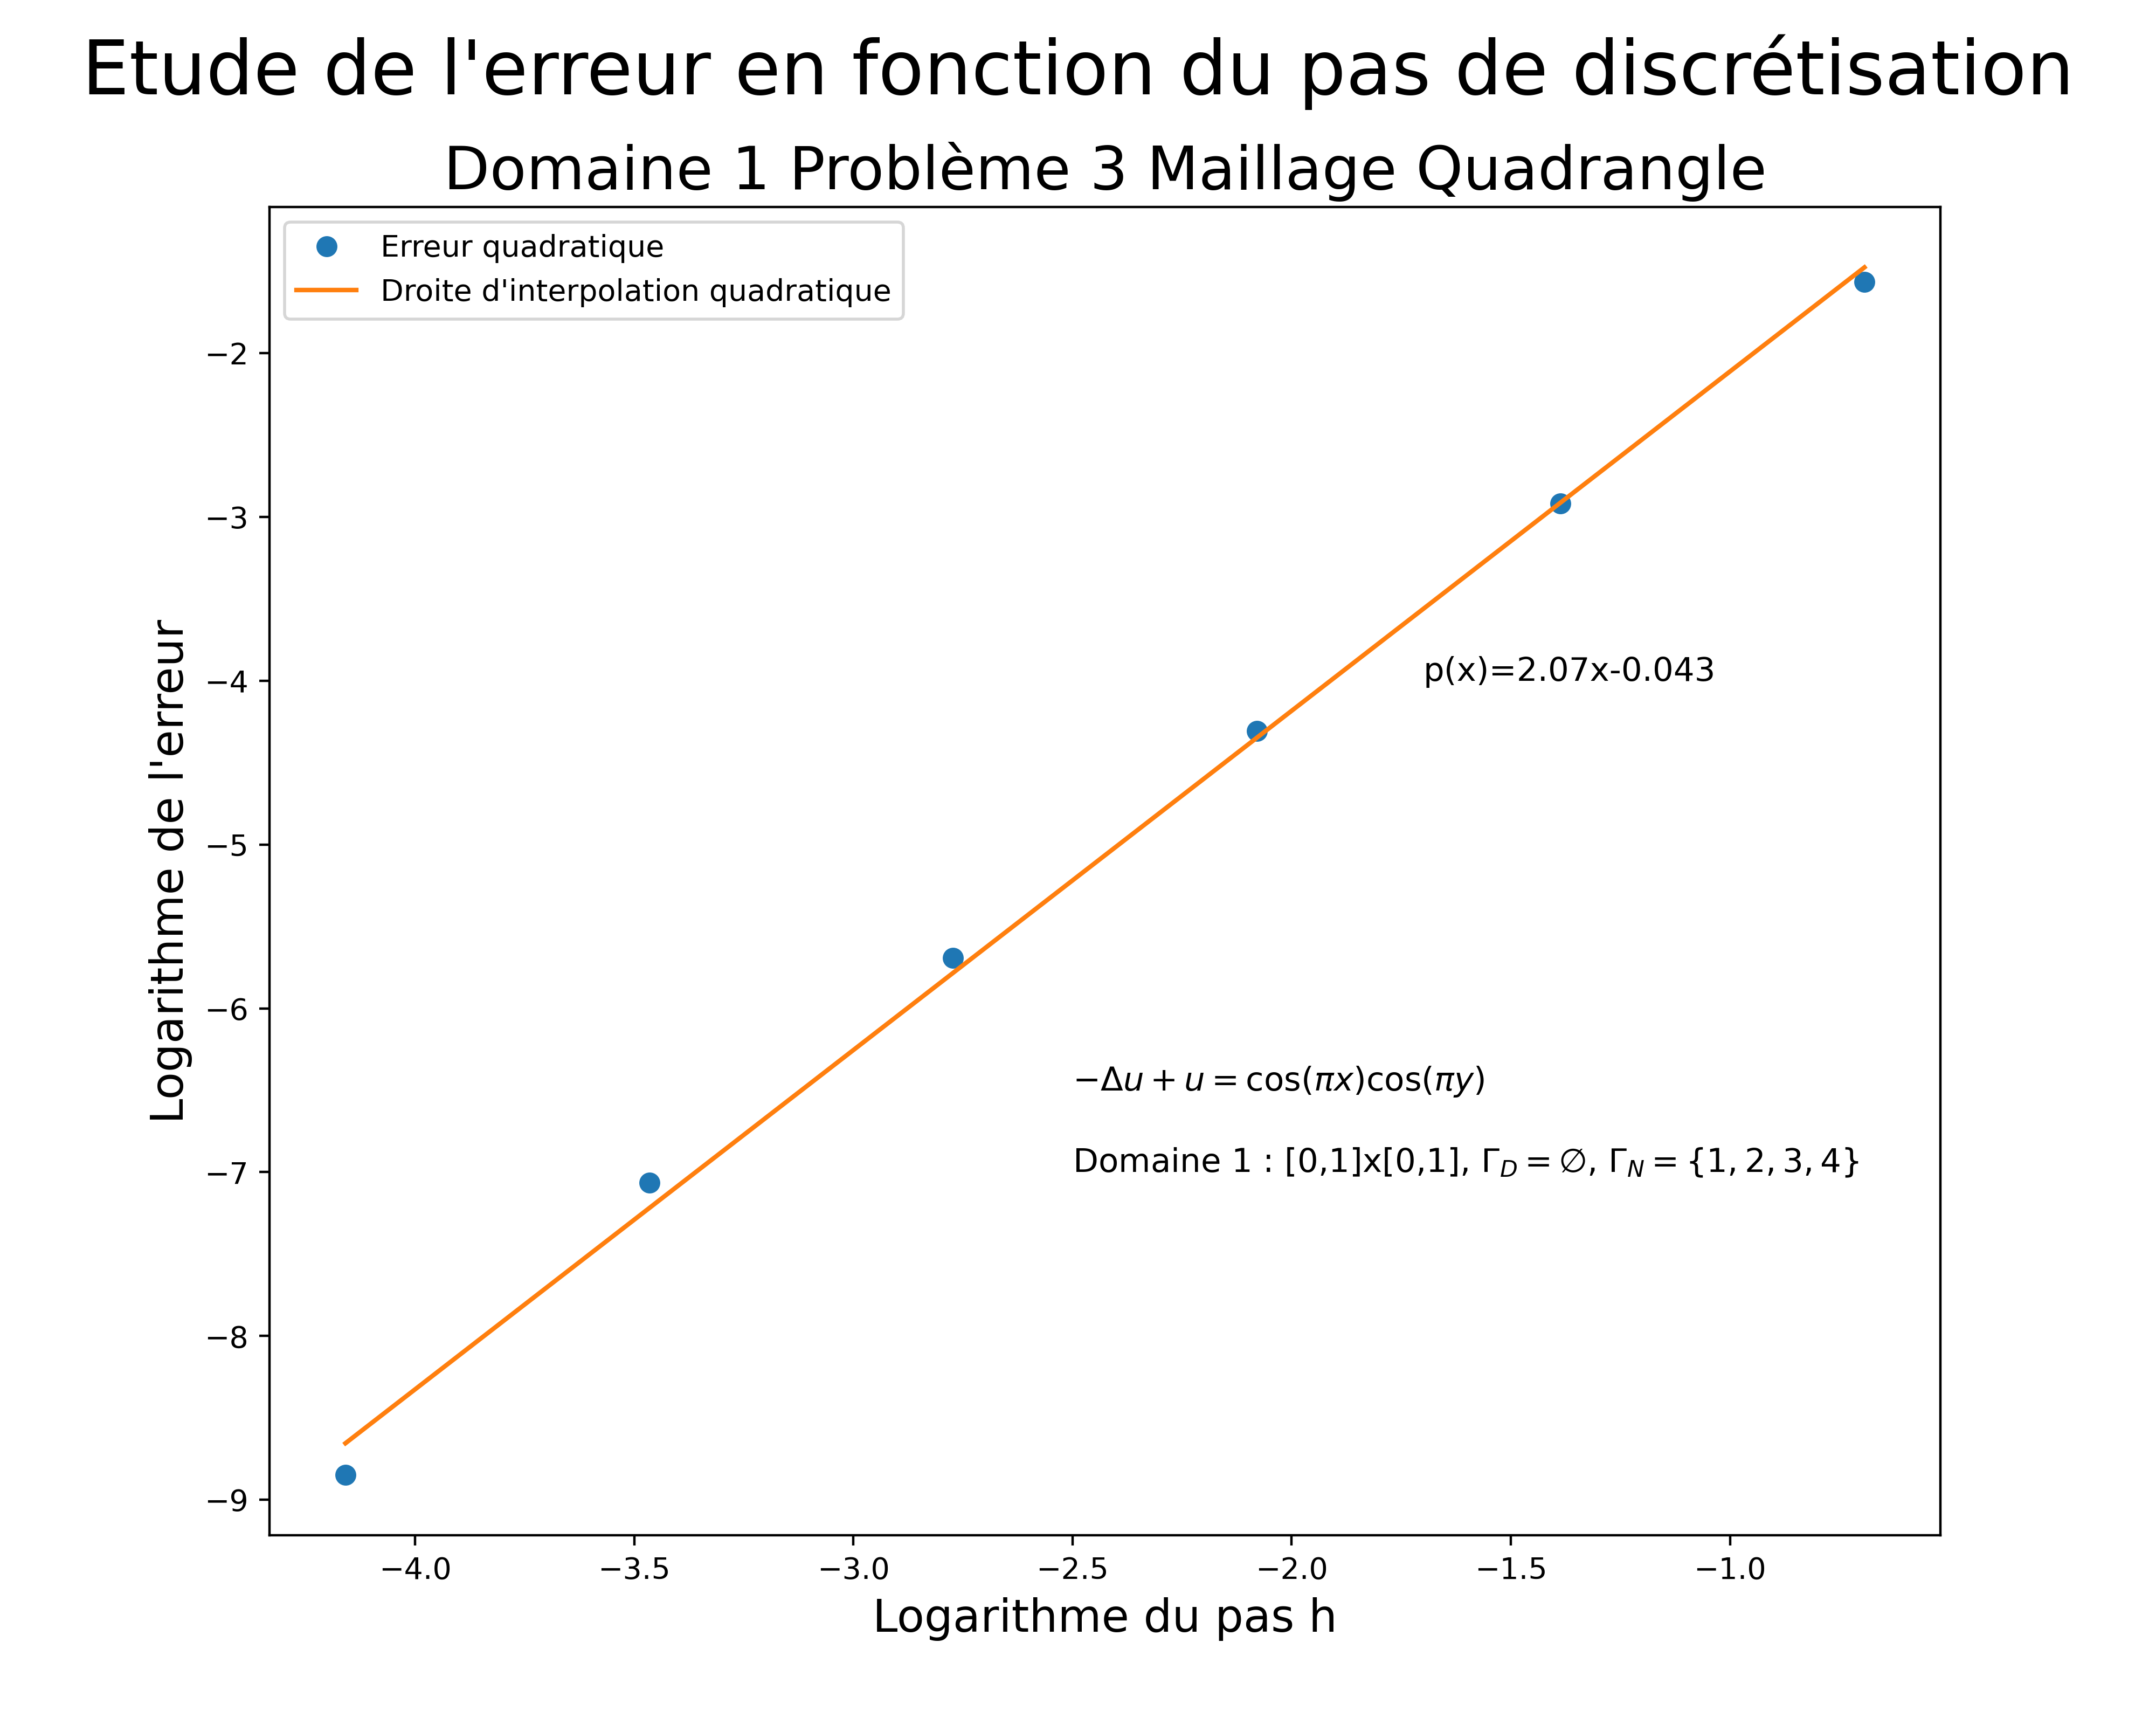
\includegraphics[height=9cm]{../Images/Courbes_Erreurs/D1P3Q.png}
\end{center}

On peut maintenant afficher la solution calculée en 3D pour visualiser la solution.
\begin{figure}[!h]
    \centering
    \begin{subfigure}{0.48\textwidth}
    	\centering
        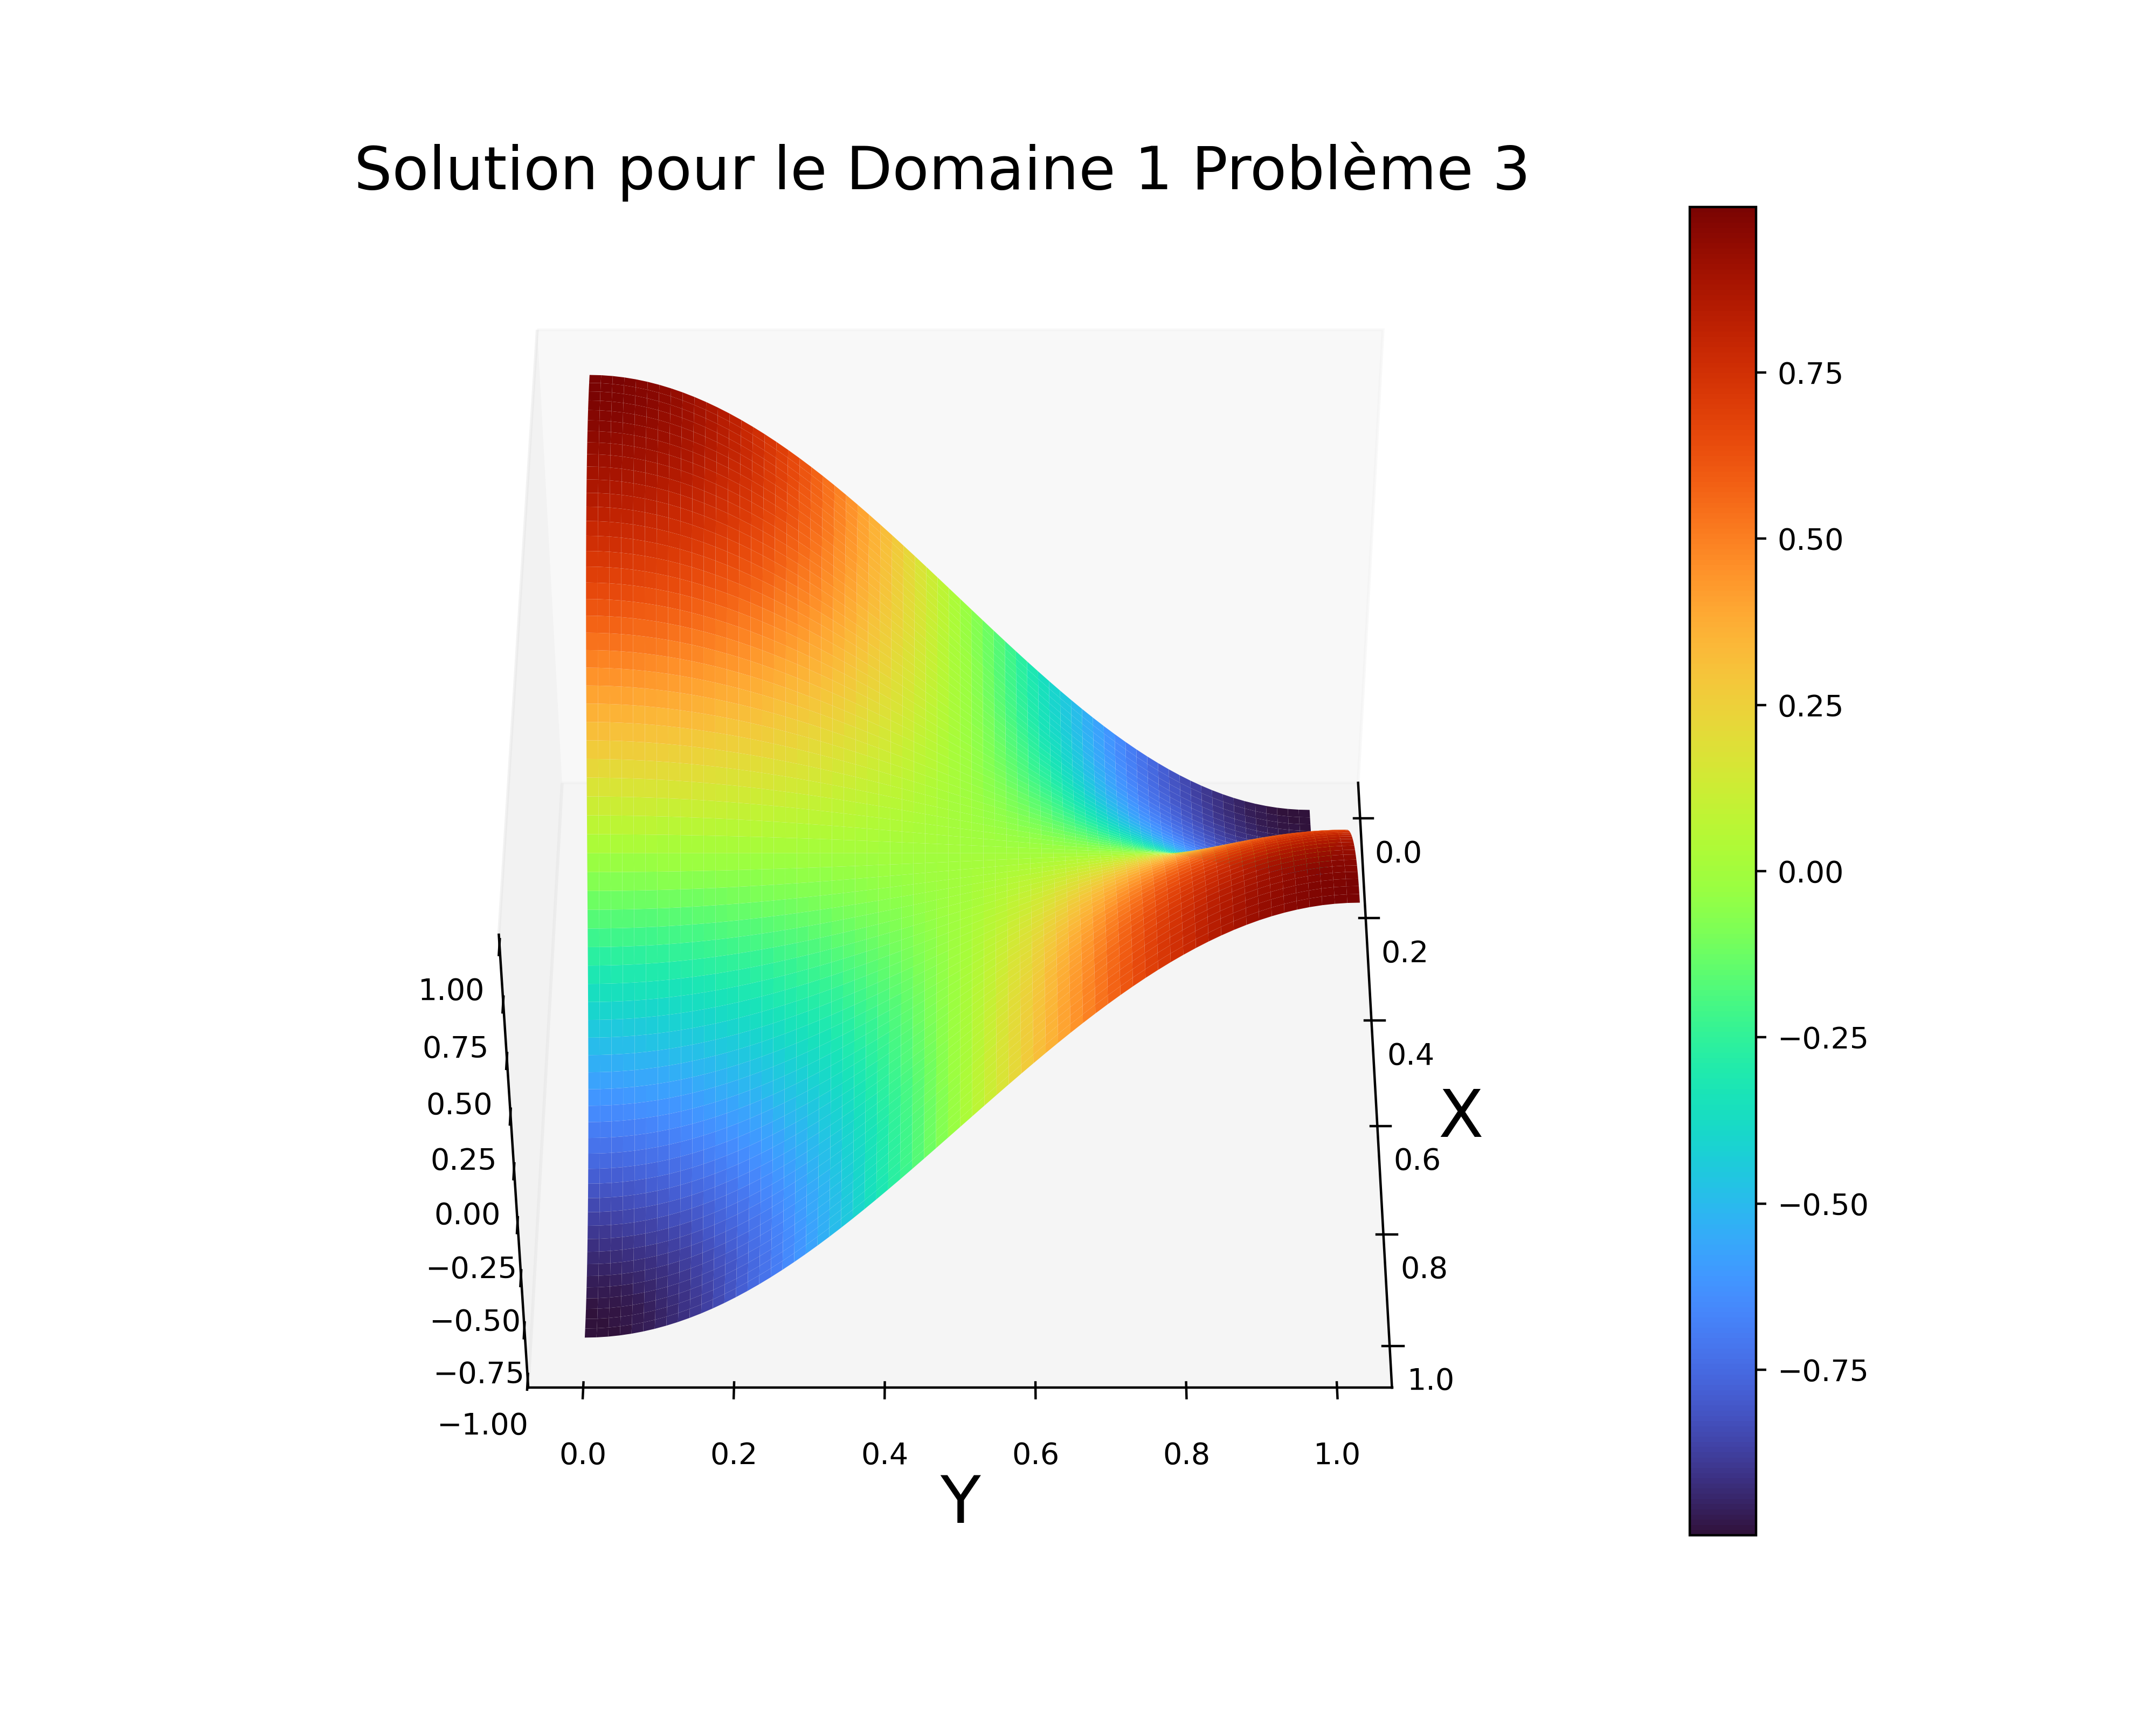
\includegraphics[height=9cm]{../Images/Figures_Calculees/sol3D13.png}
    \end{subfigure}
    \begin{subfigure}{0.48\textwidth}
    \centering
        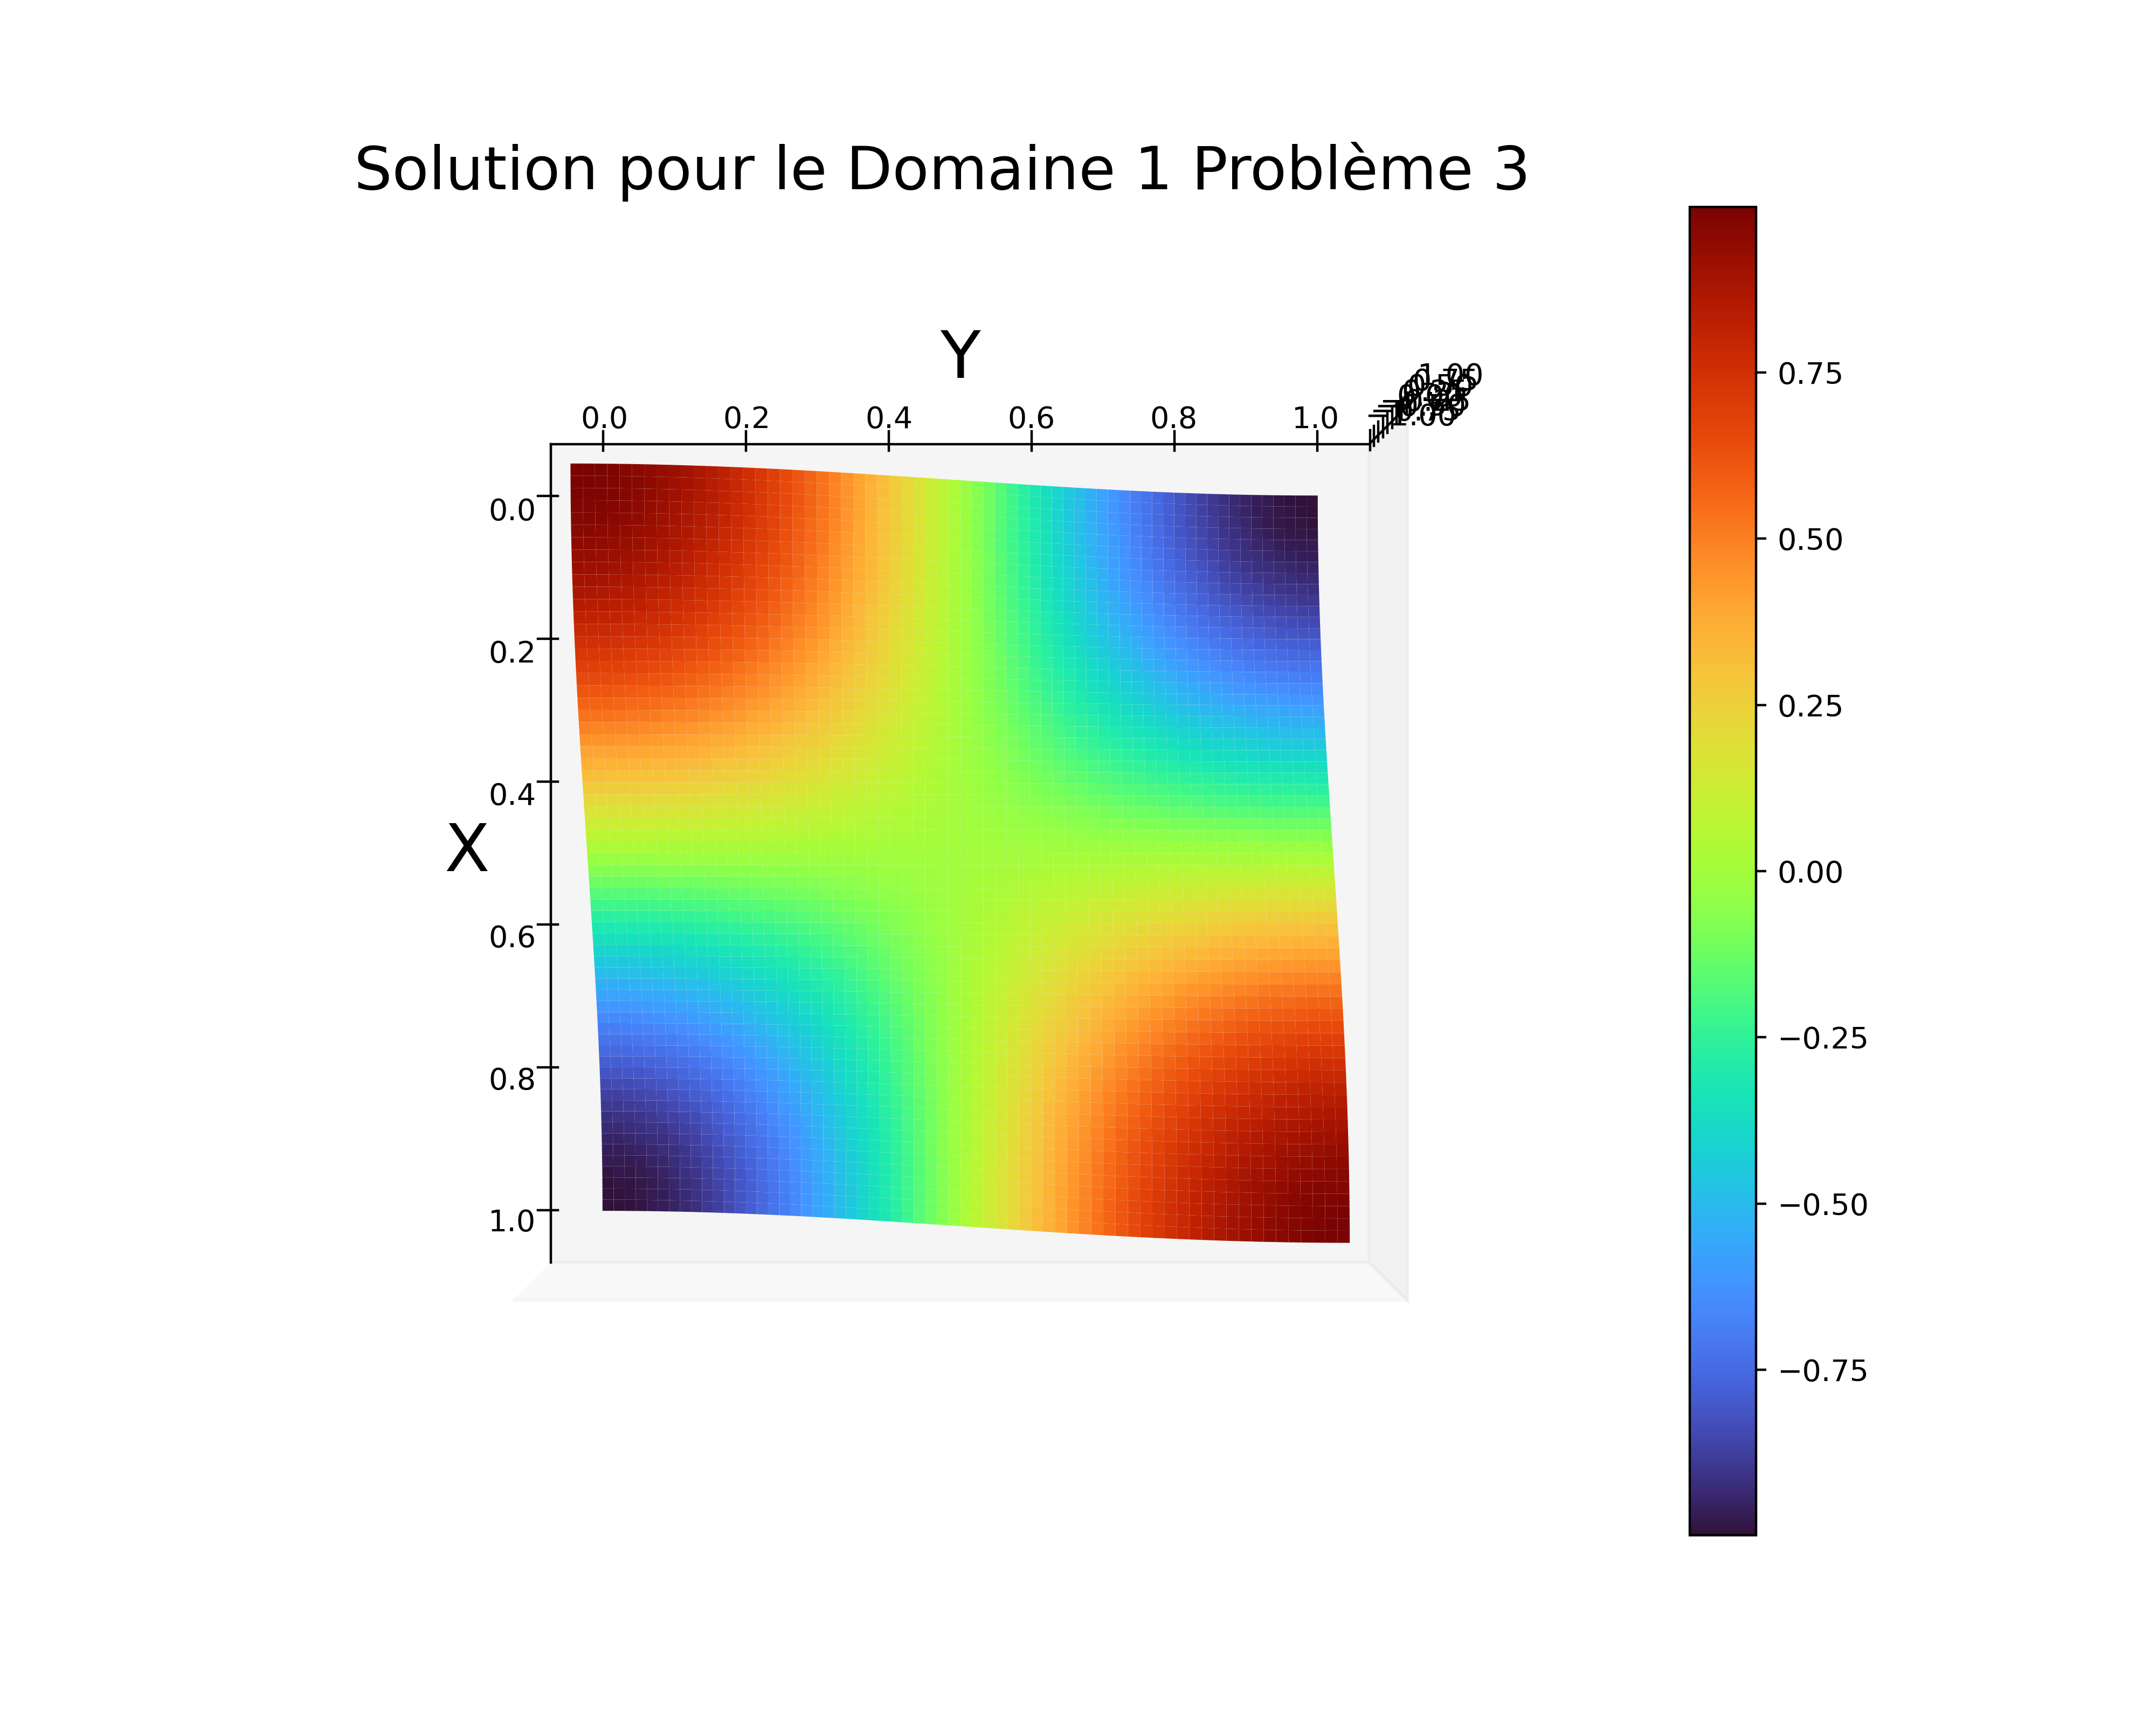
\includegraphics[height=9cm]{../Images/Figures_Calculees/sol3DVH13.png}
    \end{subfigure}
    \caption{Solution calculée vue sous différents angles Domaine 1 Problème 3 }
\end{figure}
\newpage

%%%%%%%%%%%%%%%%%%%%%%%%%%%%%%%%%
\section{Domaine 2}
%%%%%%%%%%%%%%%%%%%%%%%%%%%%%%%%%

\begin{center}
    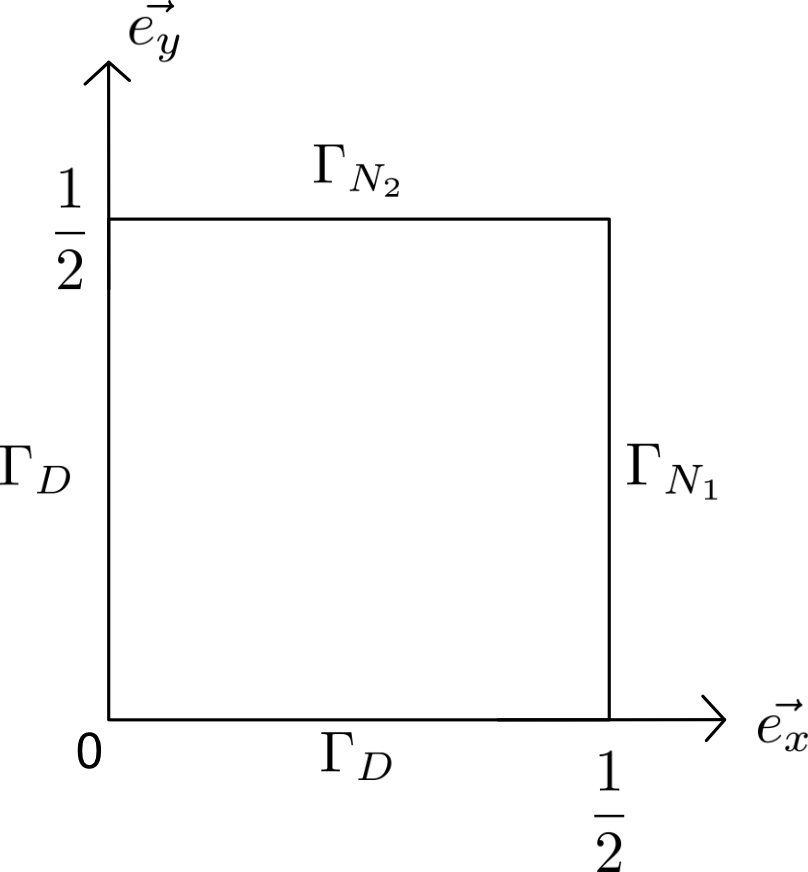
\includegraphics[height=7cm]{../Images/domaine2.png}
\end{center}

Pour le domaine 2 on a :
\begin{align*}
    \Vec{n}_{|\Gamma_{N_1}} = \Vec{e_x}\\ \Vec{n}_{|\Gamma_{N_2}}= \Vec{e_y}
\end{align*}


%%%%%%%%%%%%%%%%%%%%%%%%%%%%%%%%%
\subsection{Problème 1}
\label{D2P1}
%%%%%%%%%%%%%%%%%%%%%%%%%%%%%%%%%

Pour la solution $u=16xy(1-x)(1-y)$ :\\
On a dans un premier temps :
\begin{align*}
    \nabla u(x,y) = \Big( 16x(1-x),16y(1-y) \Big)^T
\end{align*}
On peut donc calculer $f_N$ : 

\begin{align*}
    f_N = \left\{
    \begin{array}{ll}
        16x(1-x)  \quad &\text{ sur $\Gamma_1$}\\
        16y(1-y)\quad &\text{ sur $\Gamma_2$}\\
    \end{array}
    \right.
\end{align*}
On a maintenant la définition des autres fonctions de la formulation variationelle :
\begin{align*}
    &a_{\alpha\beta} = \delta_{\alpha\beta}\\
    &a_{00} = 0\\
    &b_N = 0\\
    &f_\Omega = 32\big( x(1-x) + y(1-y) \big)\\
    &u_D = 16 x y (1-x)(1-y)
\end{align*}

On peut maintenant exécuter notre programme pour chaque maillage.
Dans un premier temps on utilise des maillages constitués de triangles, on obtient la courbe suivante :

\begin{center}
    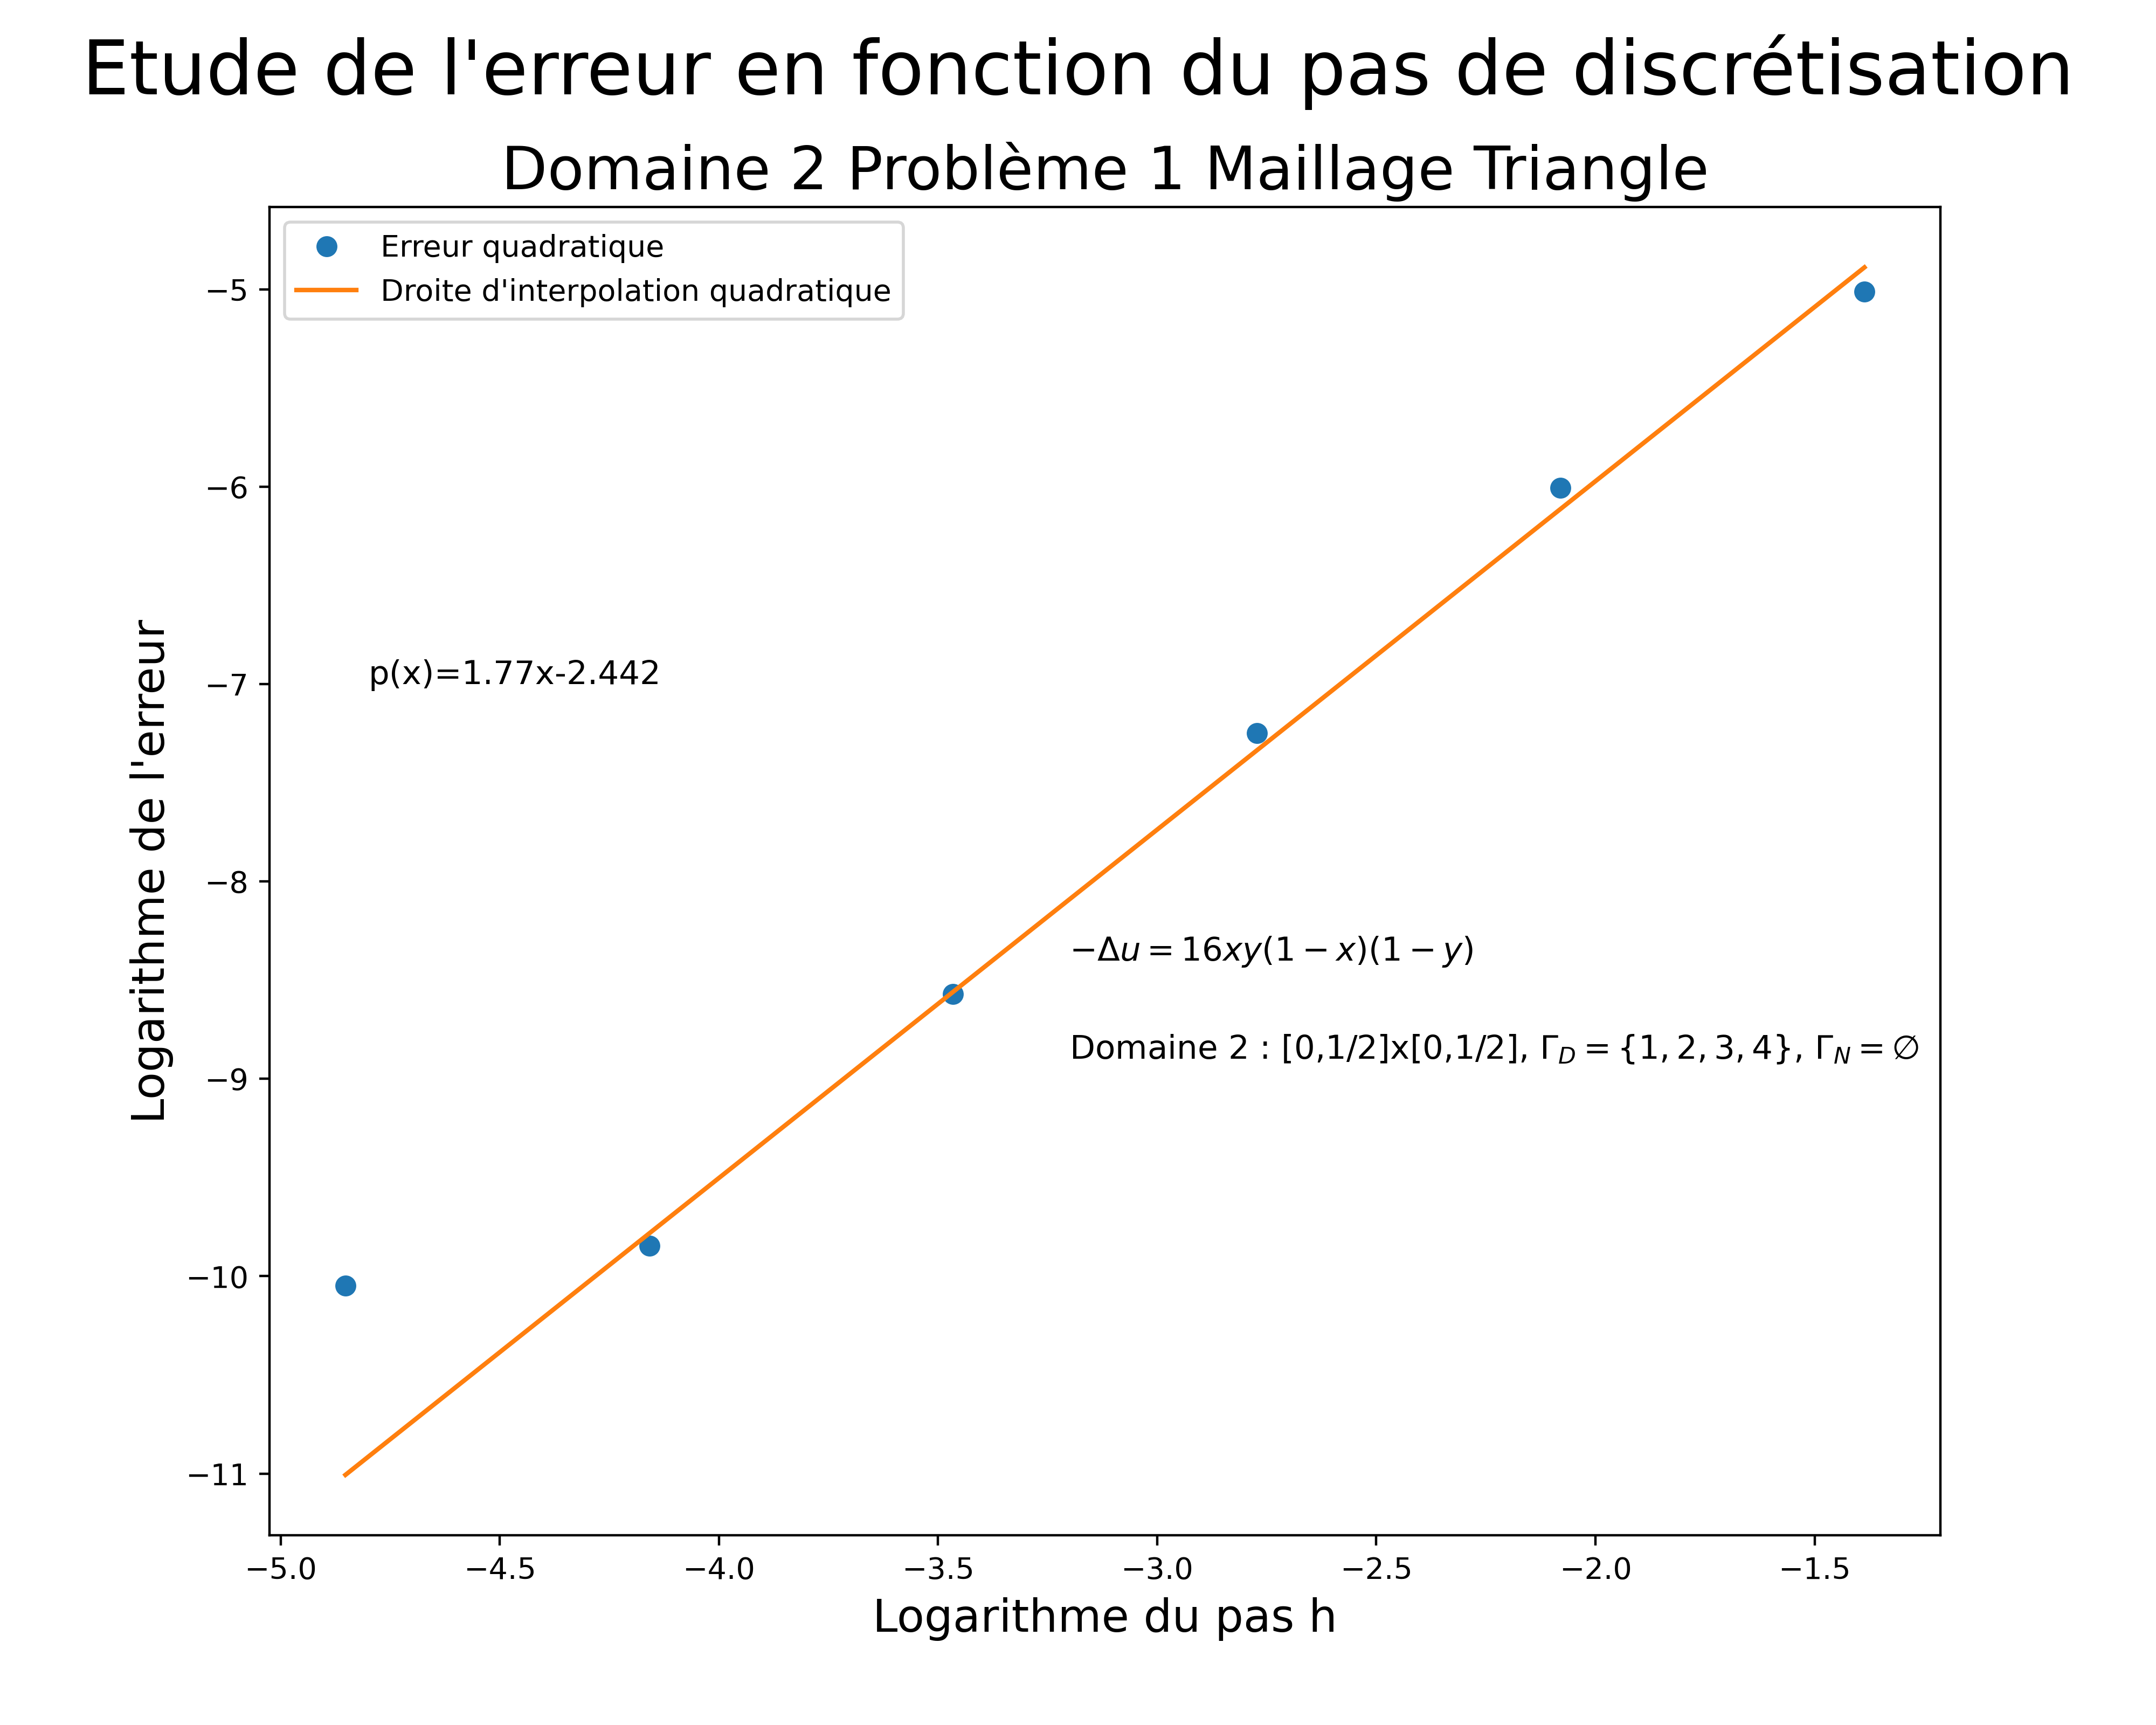
\includegraphics[height=9cm]{../Images/Courbes_Erreurs/D2P1T.png}
\end{center}

Dans un second temps, pour le même problème on utilise un maillage de quadrangle, on obtient alors la courbe suivante :
\begin{center}
    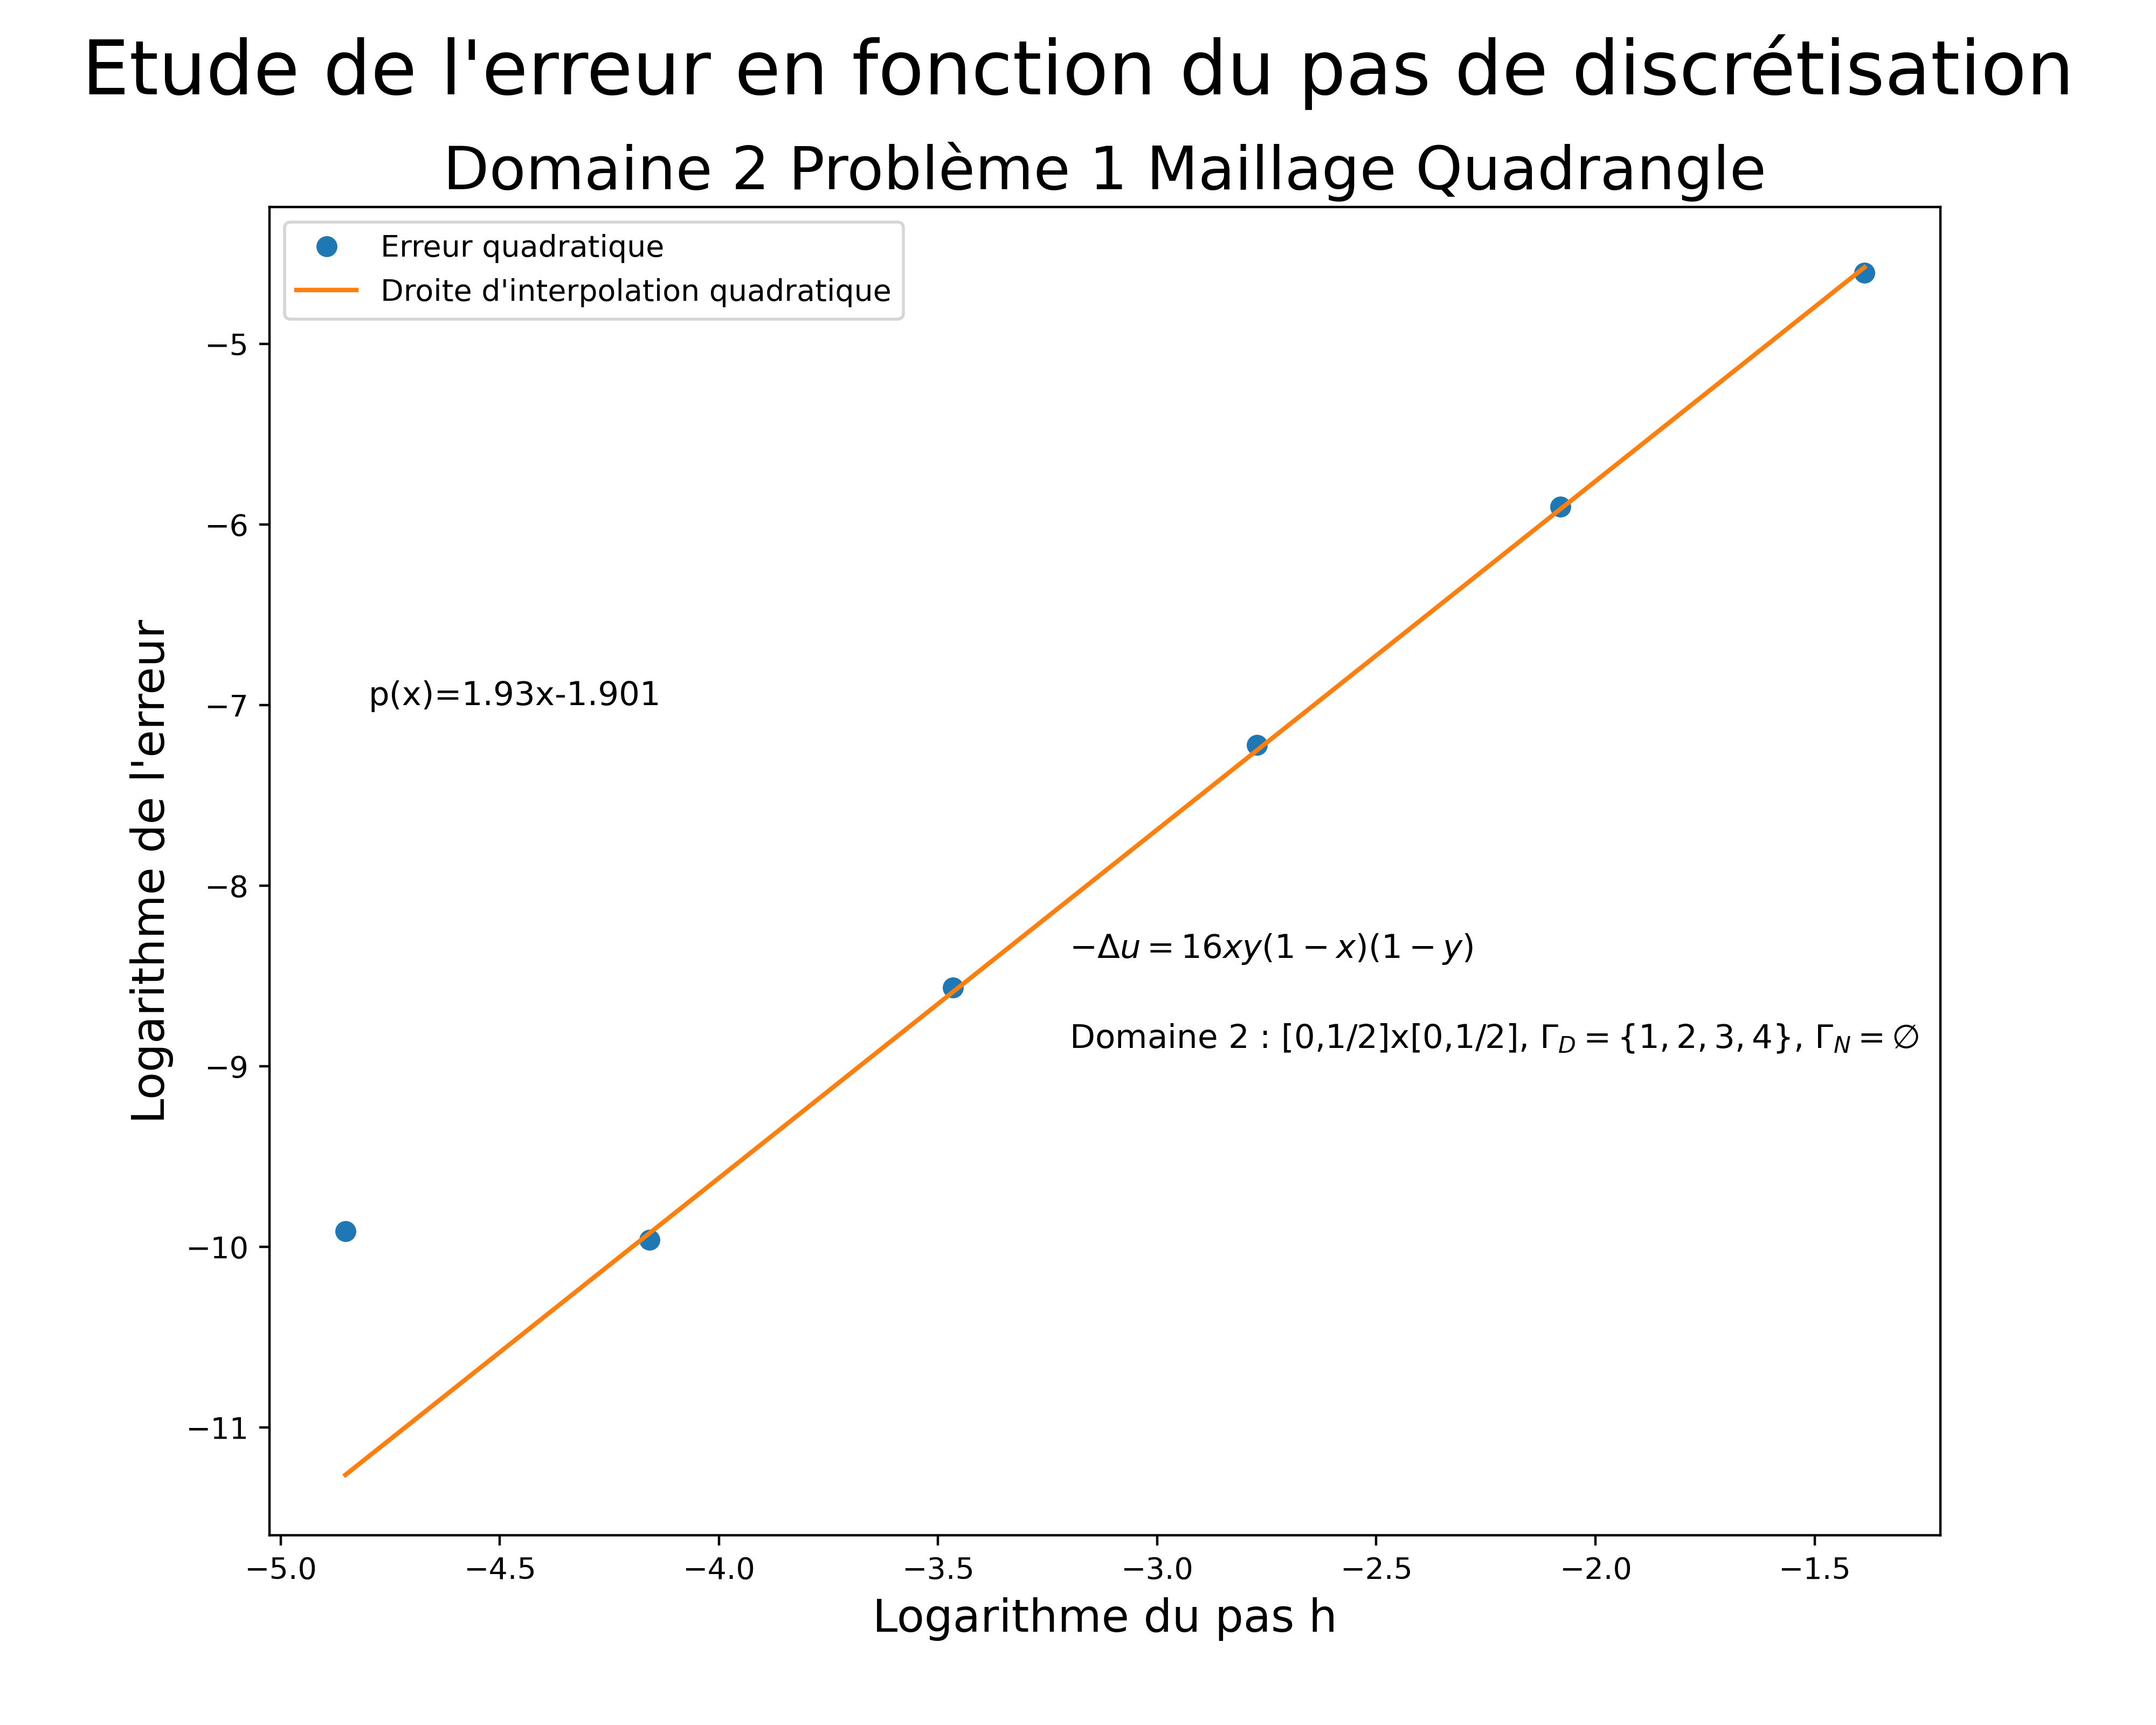
\includegraphics[height=9cm]{../Images/Courbes_Erreurs/D2P1Q.png}
\end{center}

On peut maintenant afficher la solution calculée en 3D pour visualiser la solution.
\begin{figure}[!h]
    \centering
    \begin{subfigure}{0.48\textwidth}
    	\centering
        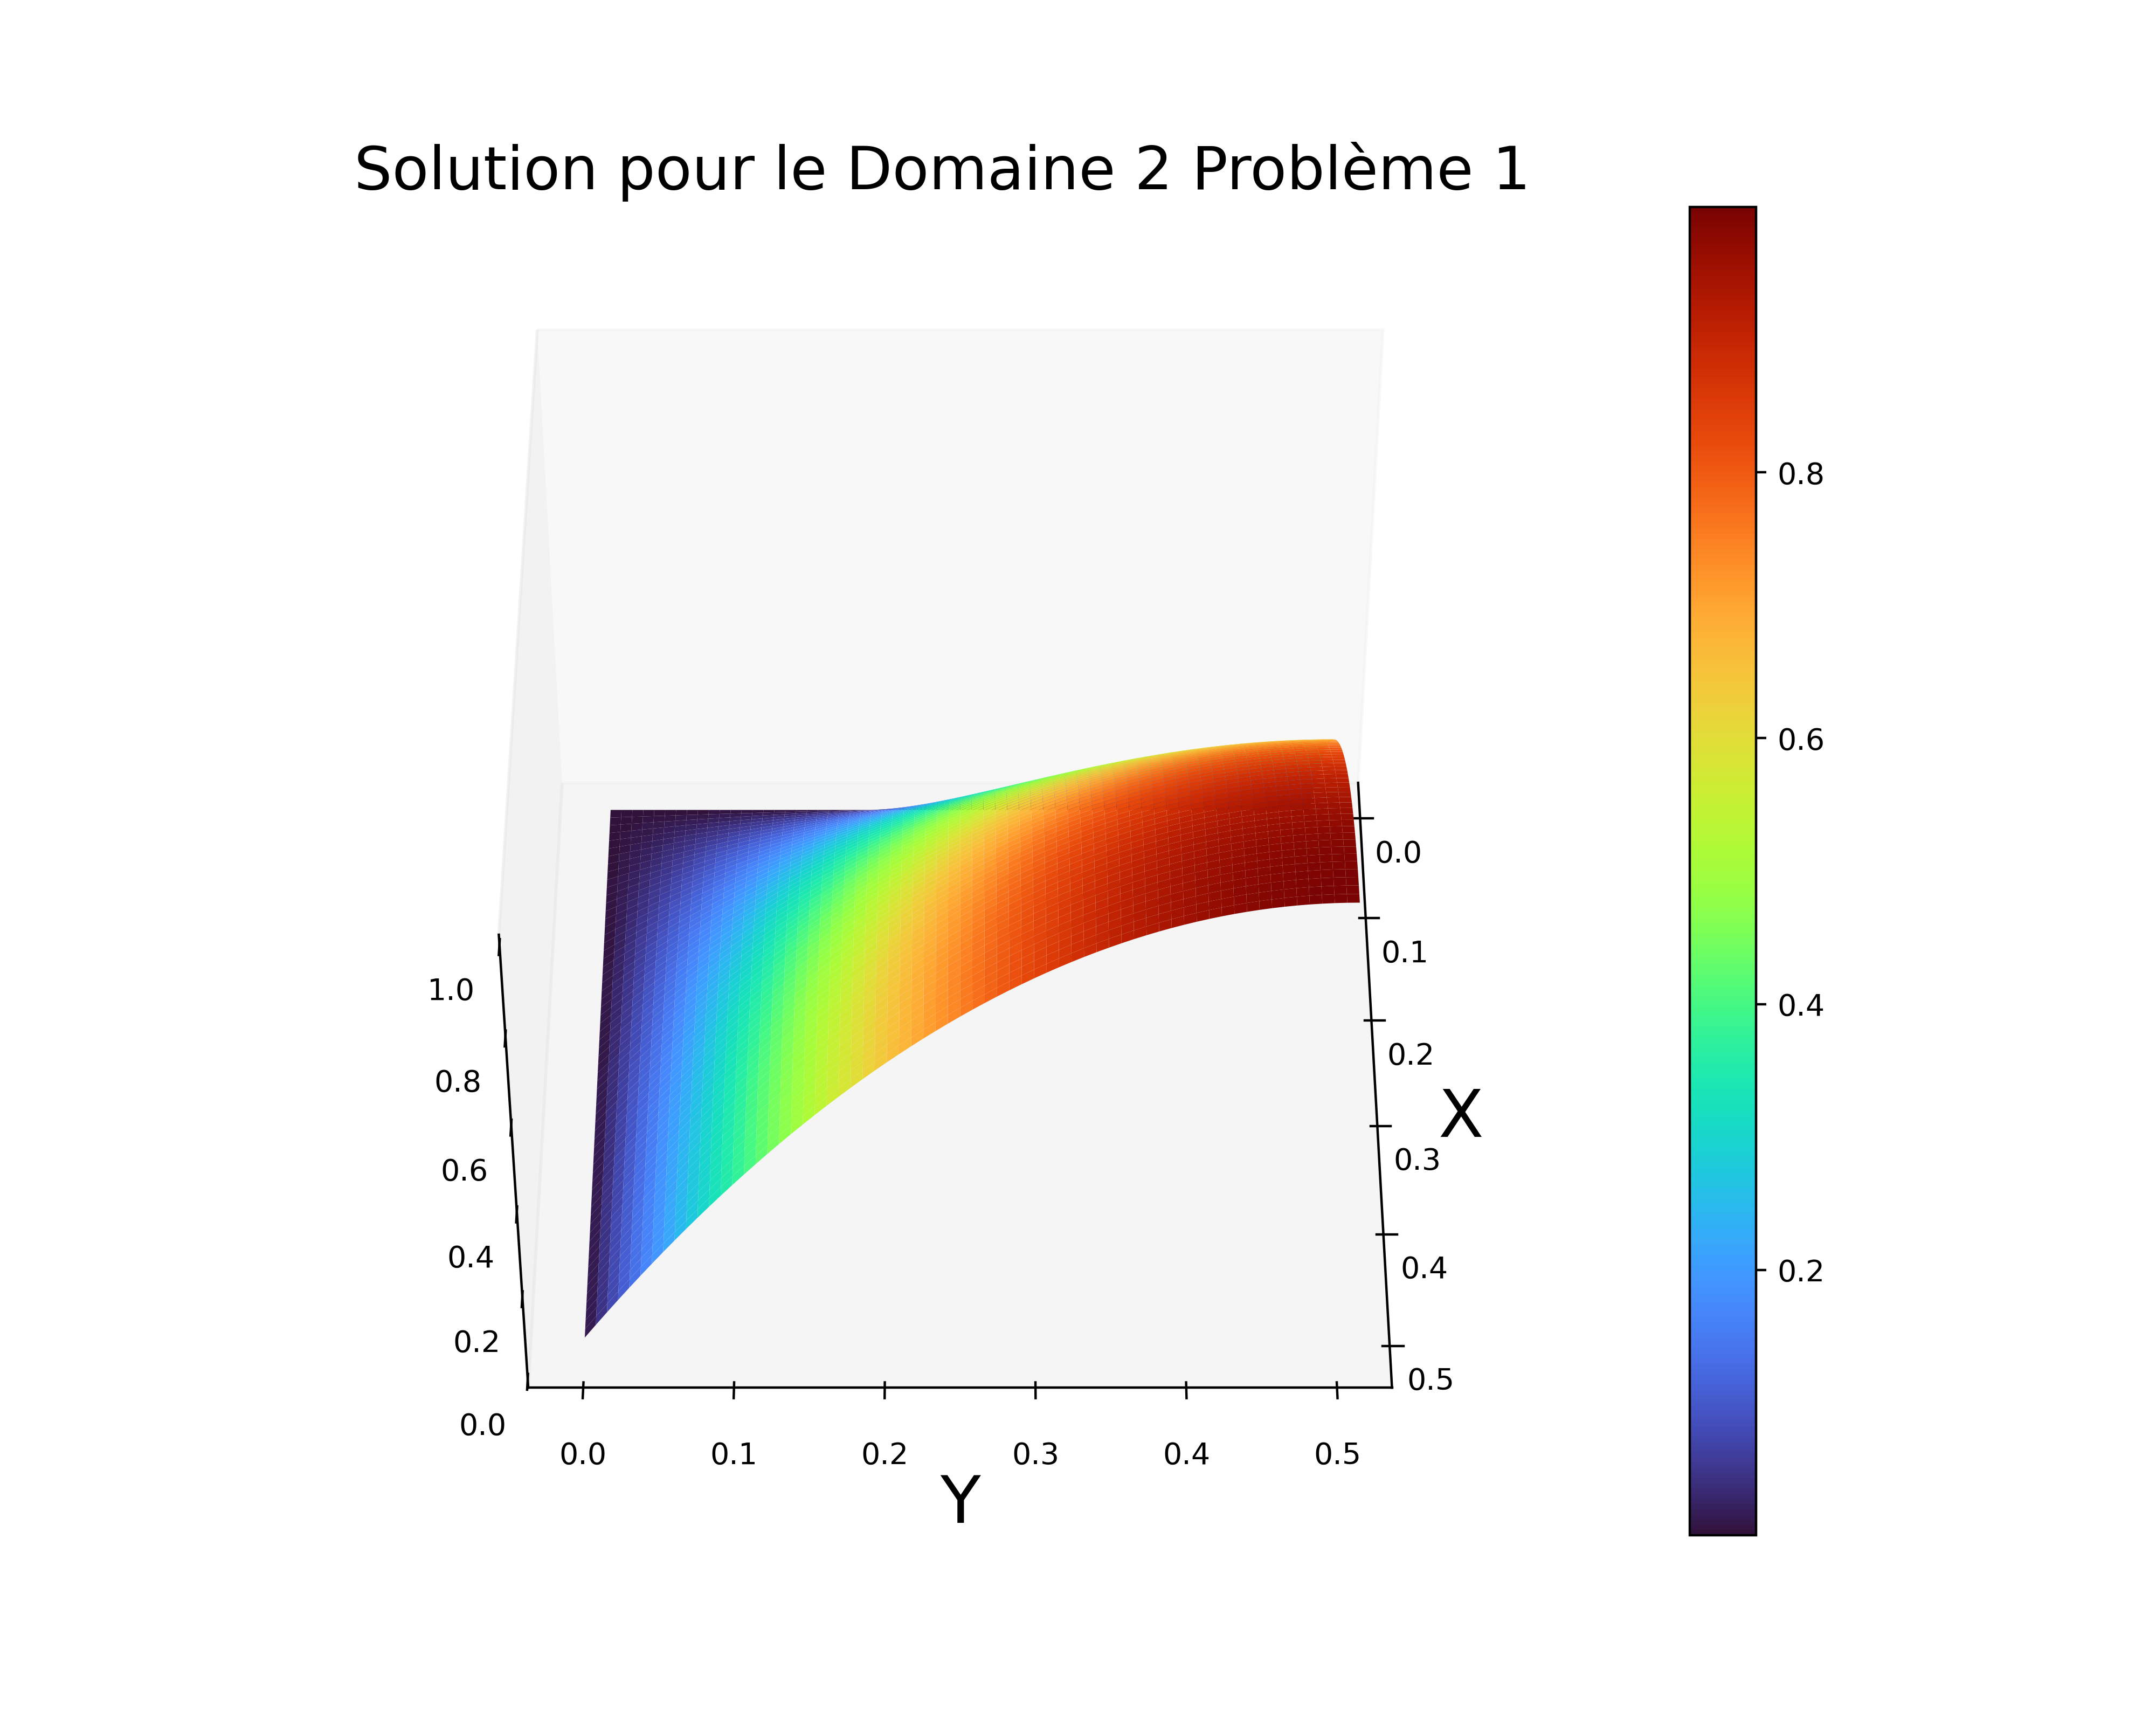
\includegraphics[height=9cm]{../Images/Figures_Calculees/sol3D21.png}
    \end{subfigure}
    \begin{subfigure}{0.48\textwidth}
    \centering
        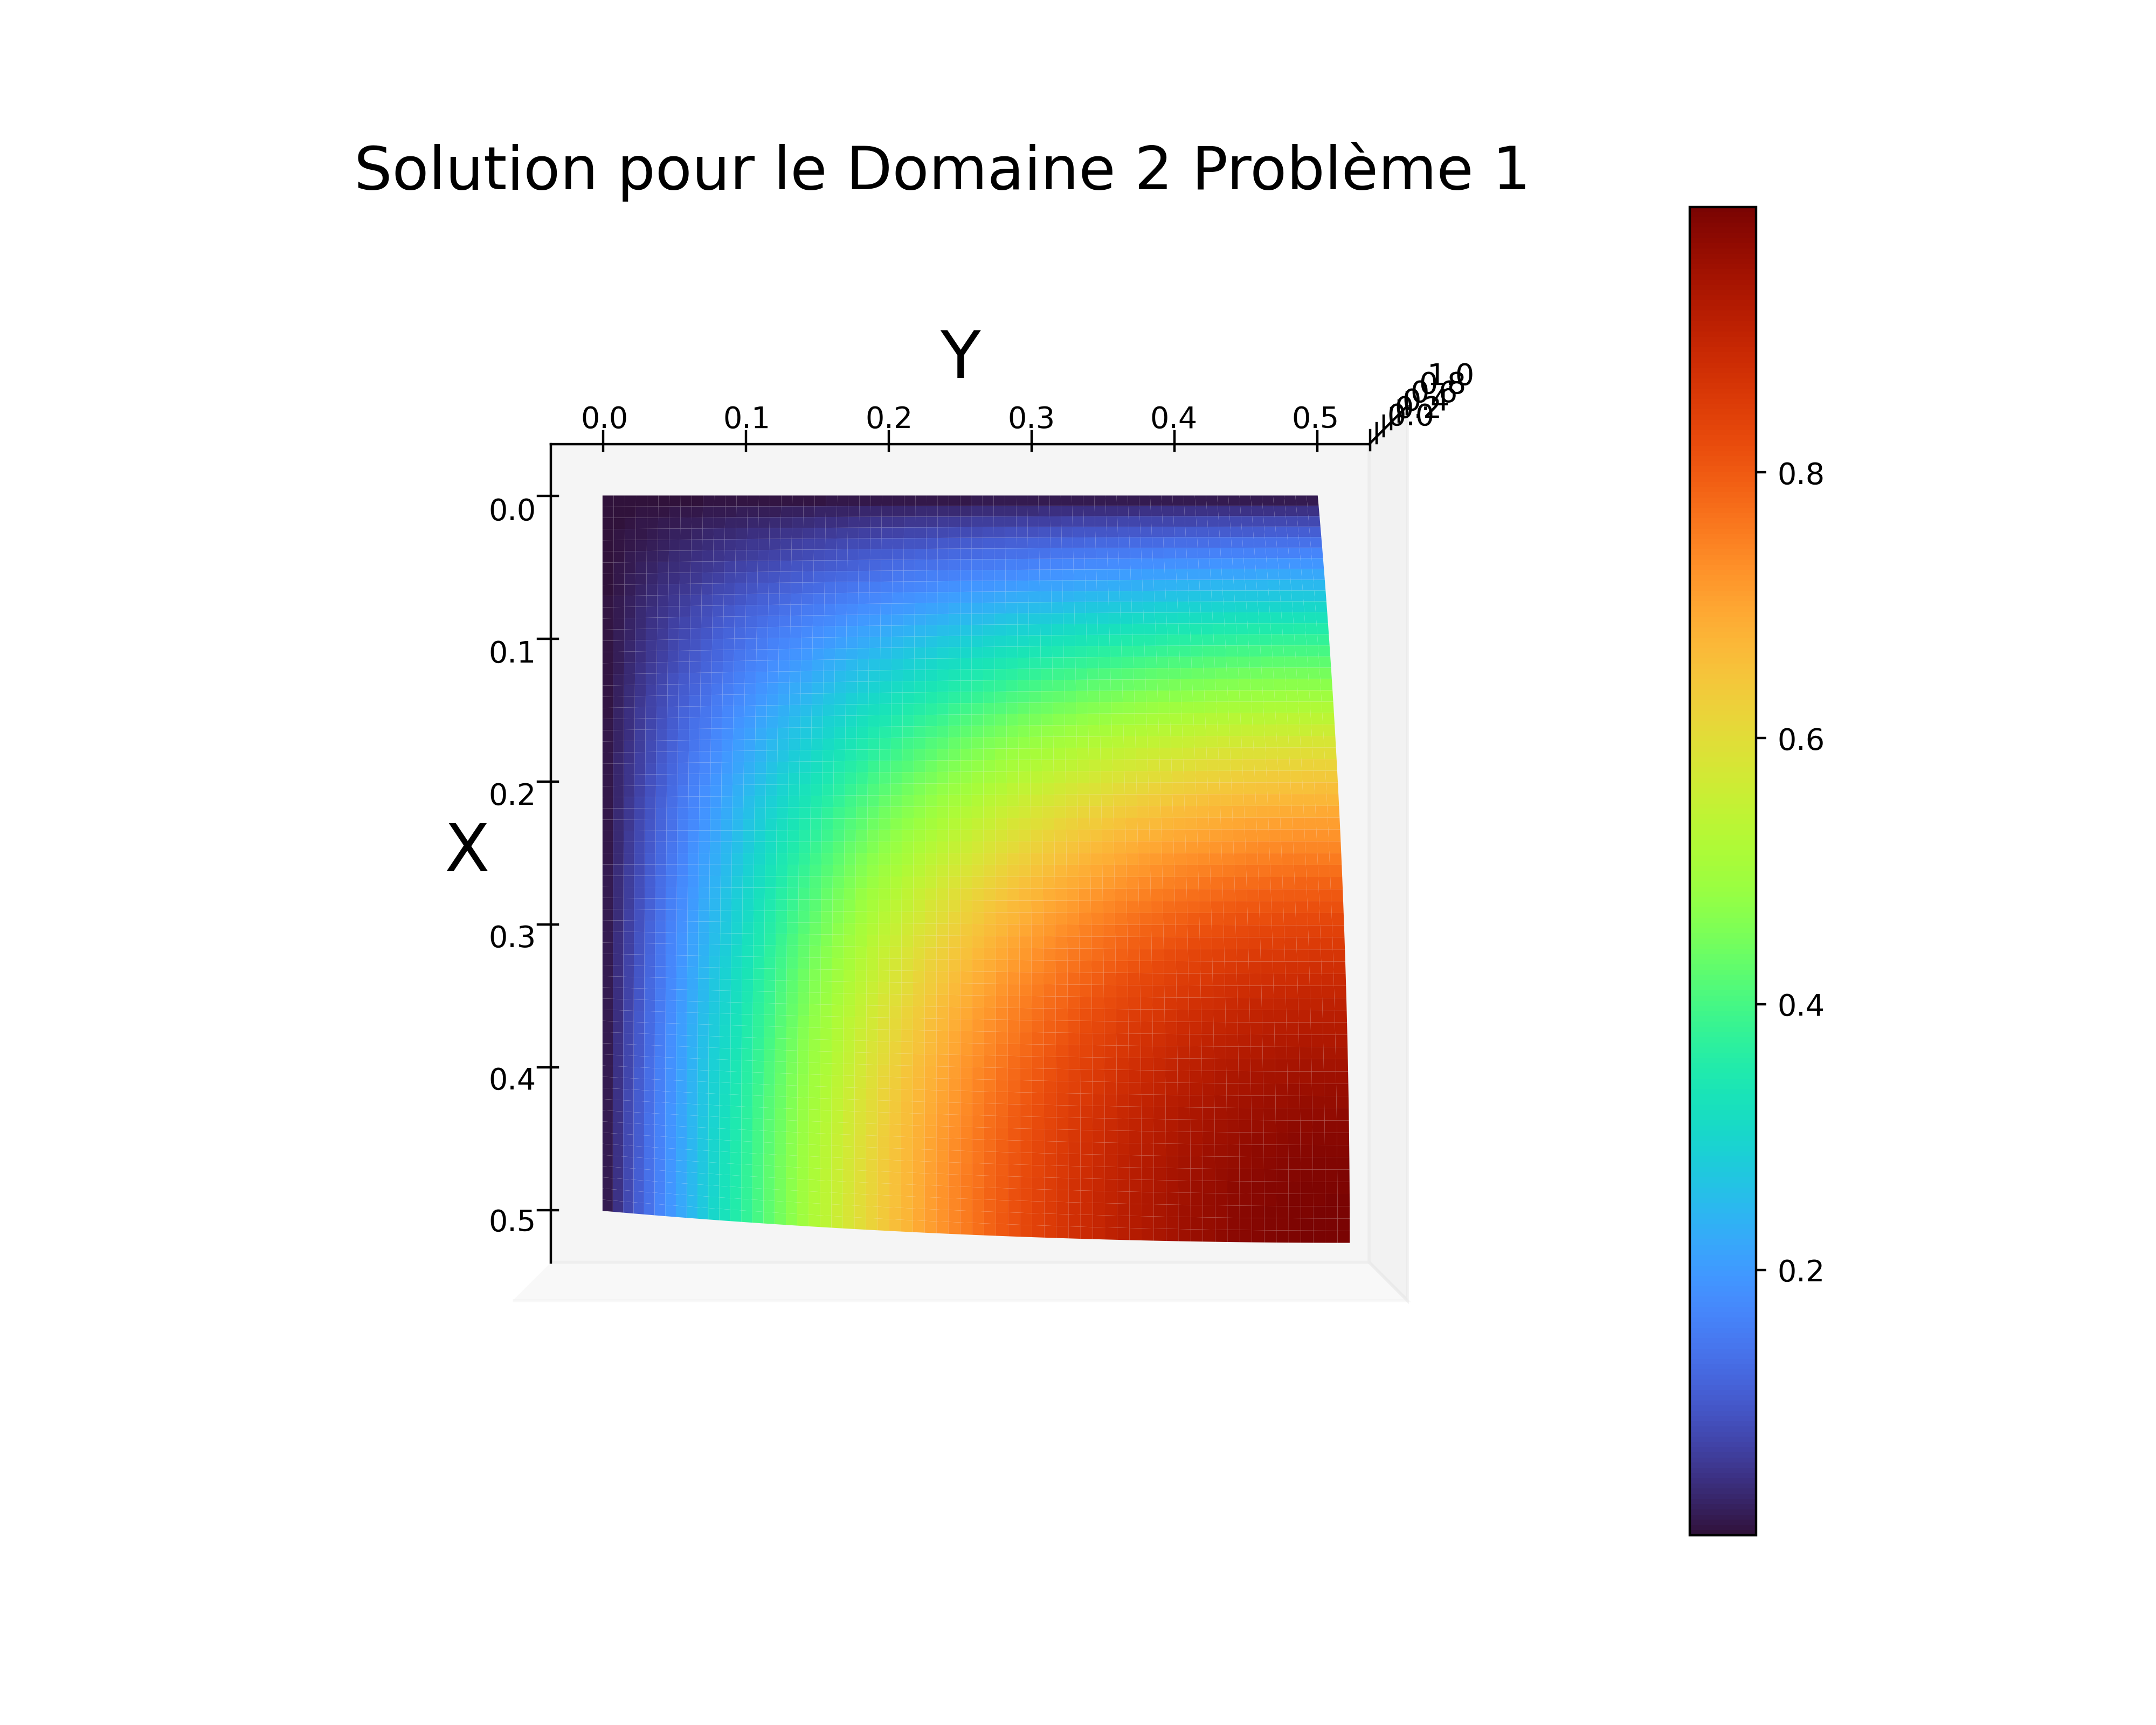
\includegraphics[height=9cm]{../Images/Figures_Calculees/sol3DVH21.png}
    \end{subfigure}
    \caption{Solution calculée vue sous différents angles Domaine 2 Problème 1 }
\end{figure}
\newpage

%%%%%%%%%%%%%%%%%%%%%%%%%%%%%%%%%
\subsection{Problème 2}
\label{D2P2}
%%%%%%%%%%%%%%%%%%%%%%%%%%%%%%%%%
Pour la solution $u=\sin(\pi x)\sin(\pi y)$ :\\
\begin{align*}
    \nabla u(x,y) = \Big( \pi\cos(\pi x)\sin(\pi y) , \pi\sin(\pi x)\cos(\pi y) \Big)^T
\end{align*}
On peut donc calculer $f_N$ :
\begin{align*}
    f_N = \left\{
    \begin{array}{ll}
        \pi\cos(\pi x)\sin(\pi y)  \quad &\text{ sur $\Gamma_1$}\\
        \pi\sin(\pi x)\cos(\pi y)\quad &\text{ sur $\Gamma_2$}\\
    \end{array}
    \right.
\end{align*}
Ici encore on a toujours la définition des autres fonctions :
\begin{align*}
    &a_{\alpha\beta} = \delta_{\alpha\beta}\\
    &a_{00} = 0\\
    &b_N = 0\\
    &u_D = \sin(\pi x)\sin(\pi y)\\
    & f_\Omega = 2\pi^2\sin(\pi x)\sin(\pi y)
\end{align*}

On peut maintenant exécuter notre programme pour chaque maillage.
Dans un premier temps on utilise des maillages constitué de triangles, on obtient la courbe suivante :

\begin{center}
    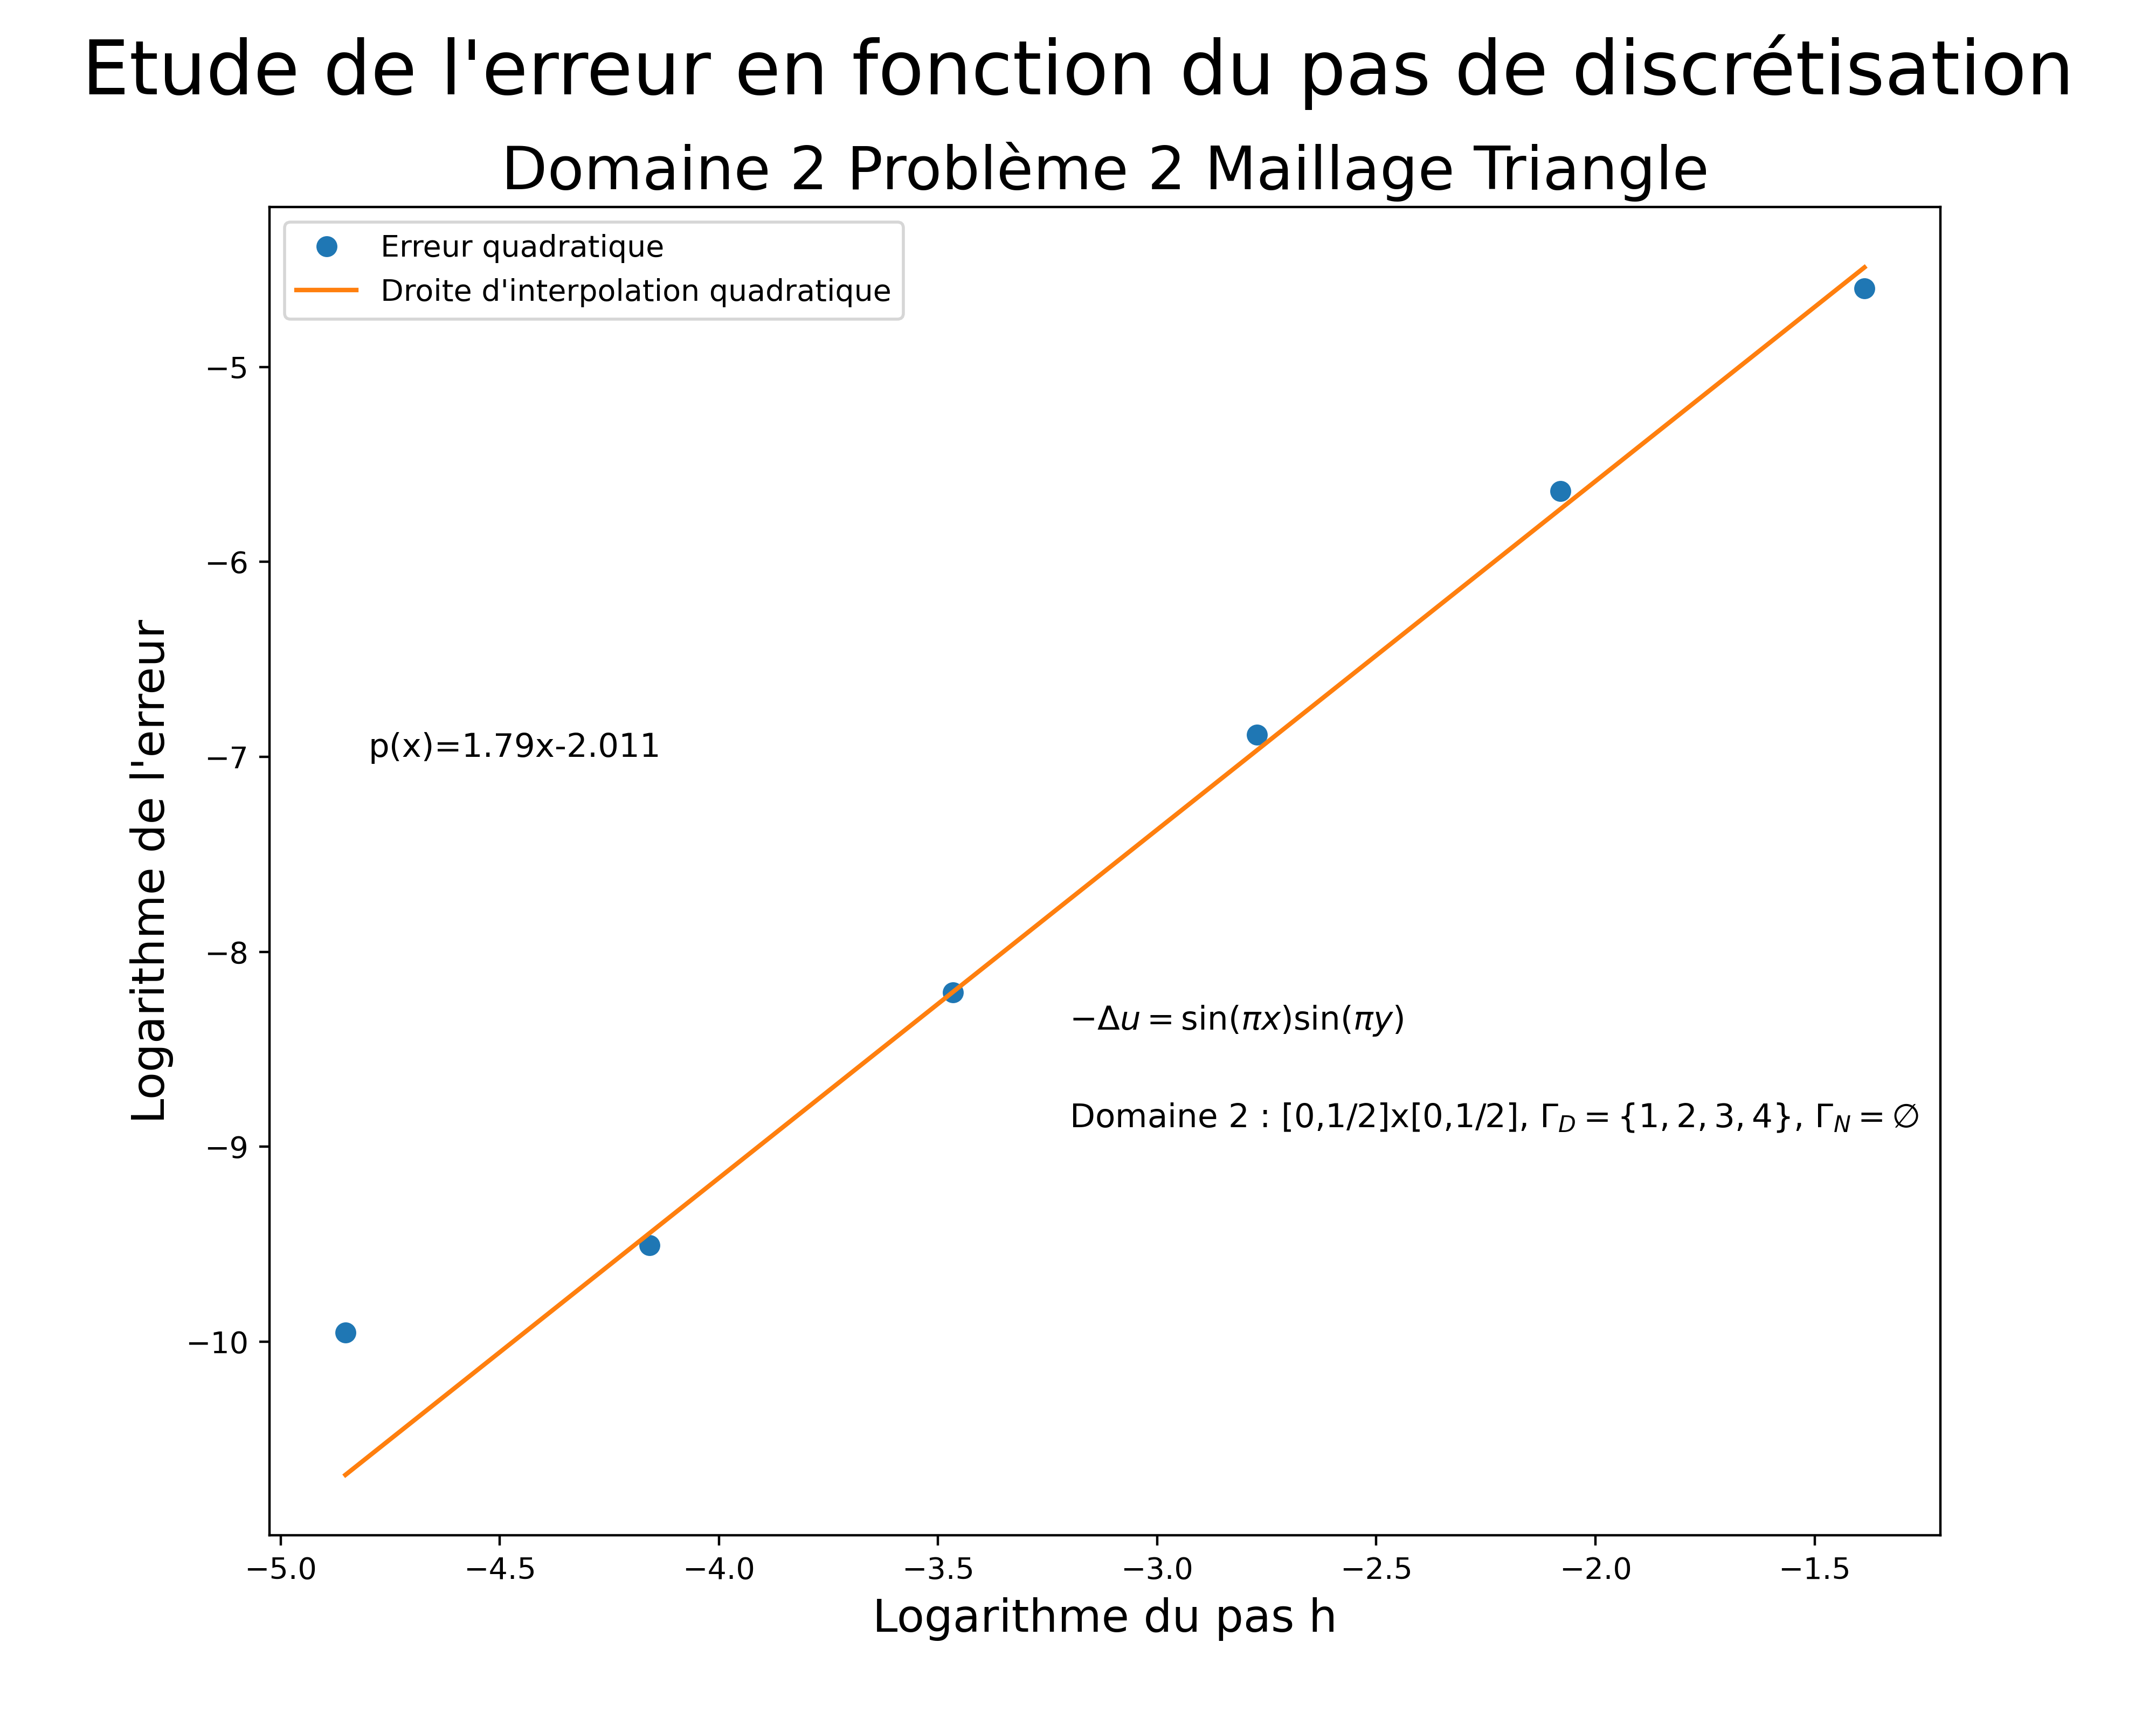
\includegraphics[height=9cm]{../Images/Courbes_Erreurs/D2P2T.png}
\end{center}

Dans un second temps, pour le même problème on utilise un maillage de quadrangle, on obtient alors la courbe suivante :
\begin{center}
    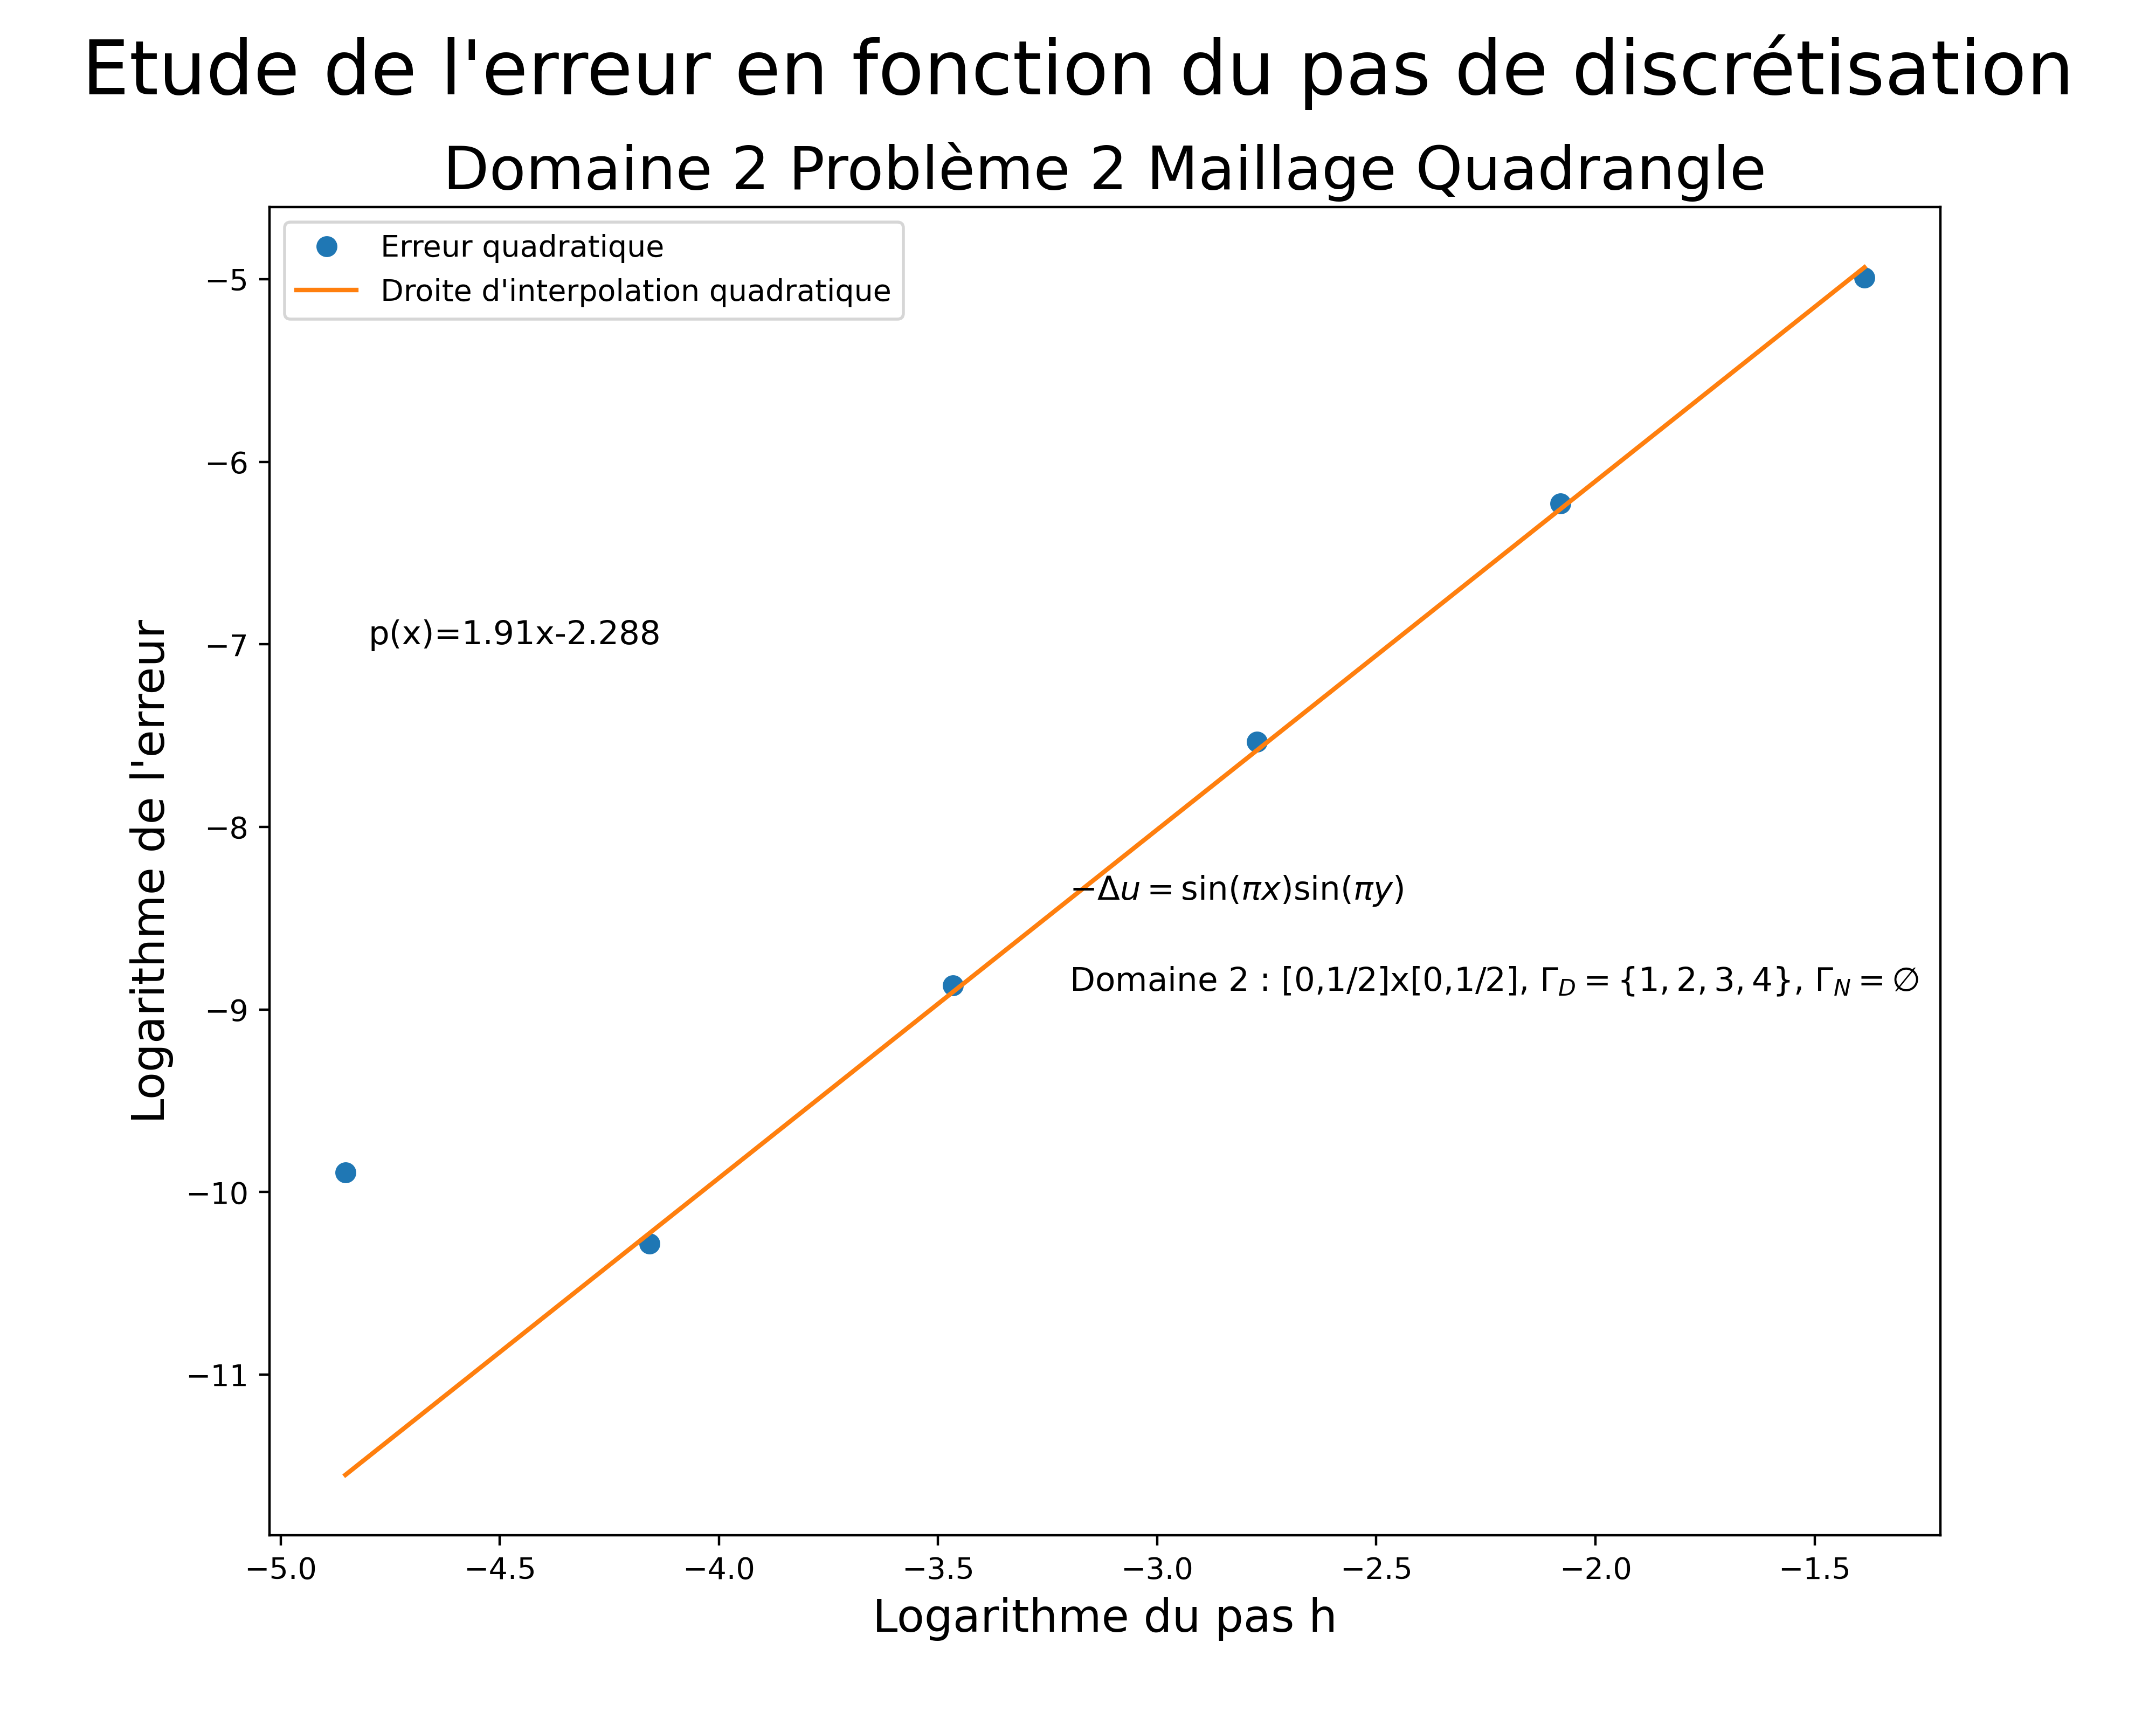
\includegraphics[height=9cm]{../Images/Courbes_Erreurs/D2P2Q.png}
\end{center}

On peut maintenant afficher la solution calculée en 3D pour visualiser la solution.
\begin{figure}[!h]
    \centering
    \begin{subfigure}{0.48\textwidth}
    	\centering
        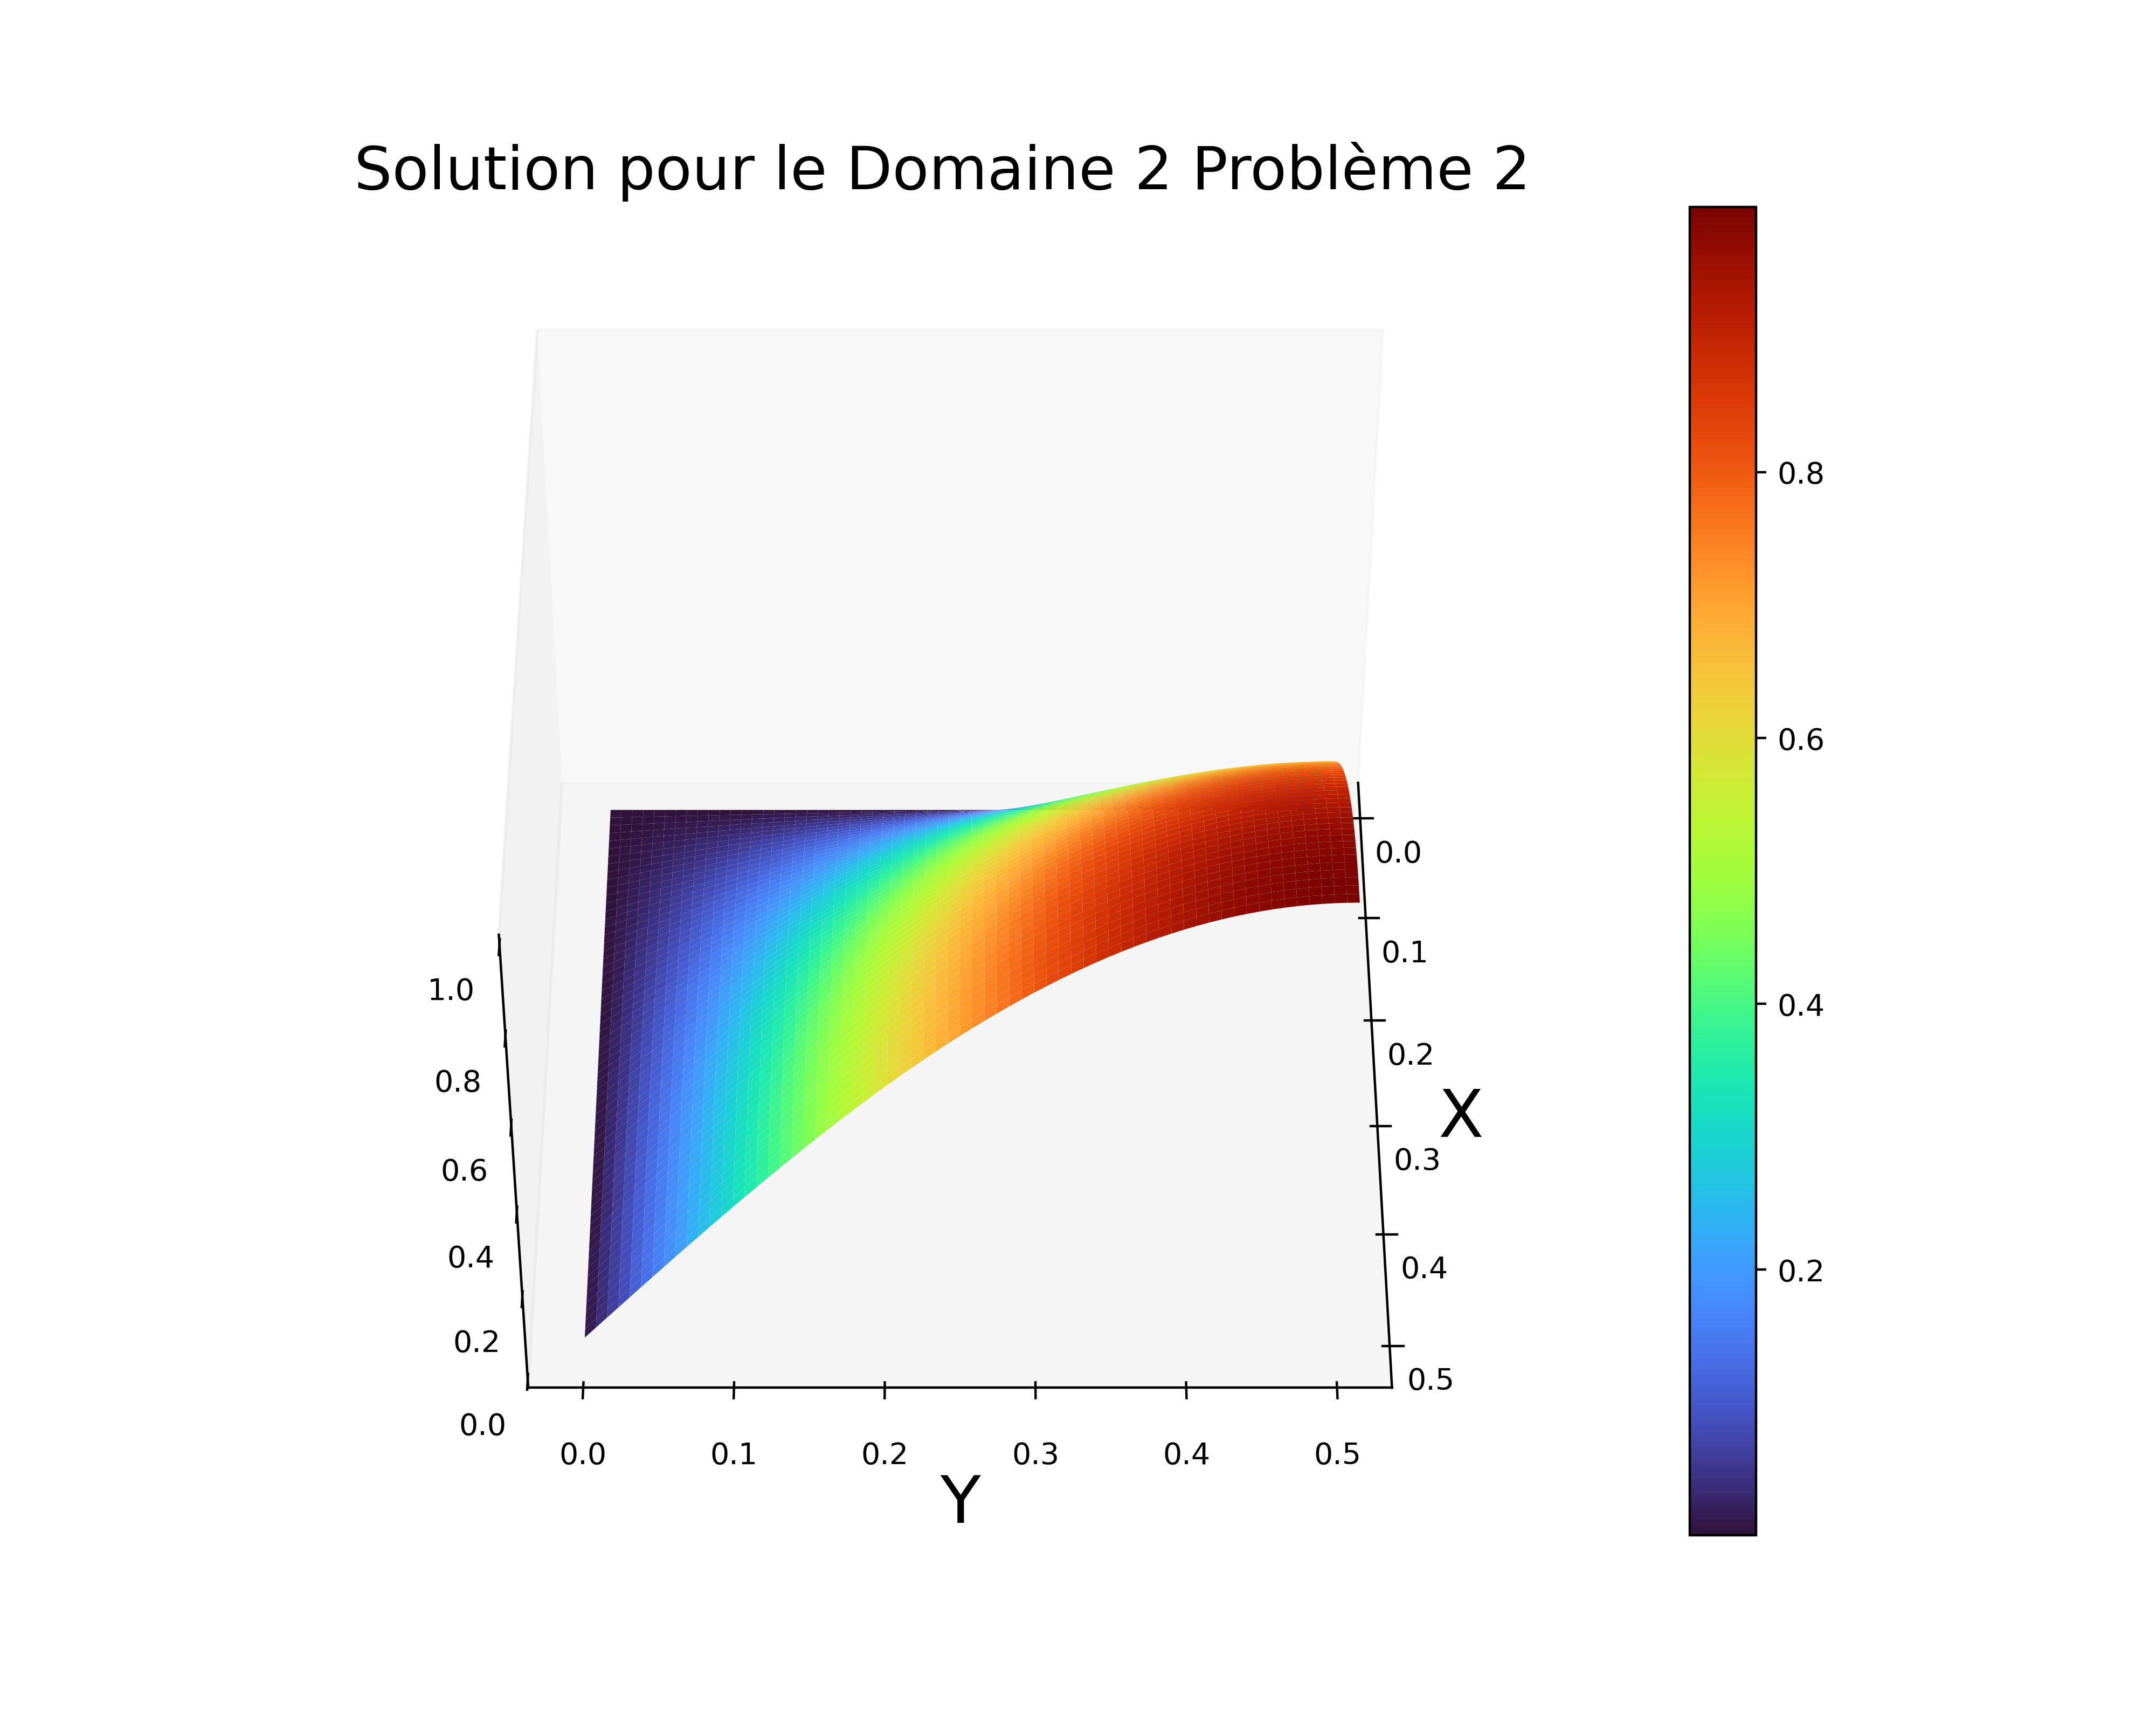
\includegraphics[height=9cm]{../Images/Figures_Calculees/sol3D22.png}
    \end{subfigure}
    \begin{subfigure}{0.48\textwidth}
    \centering
        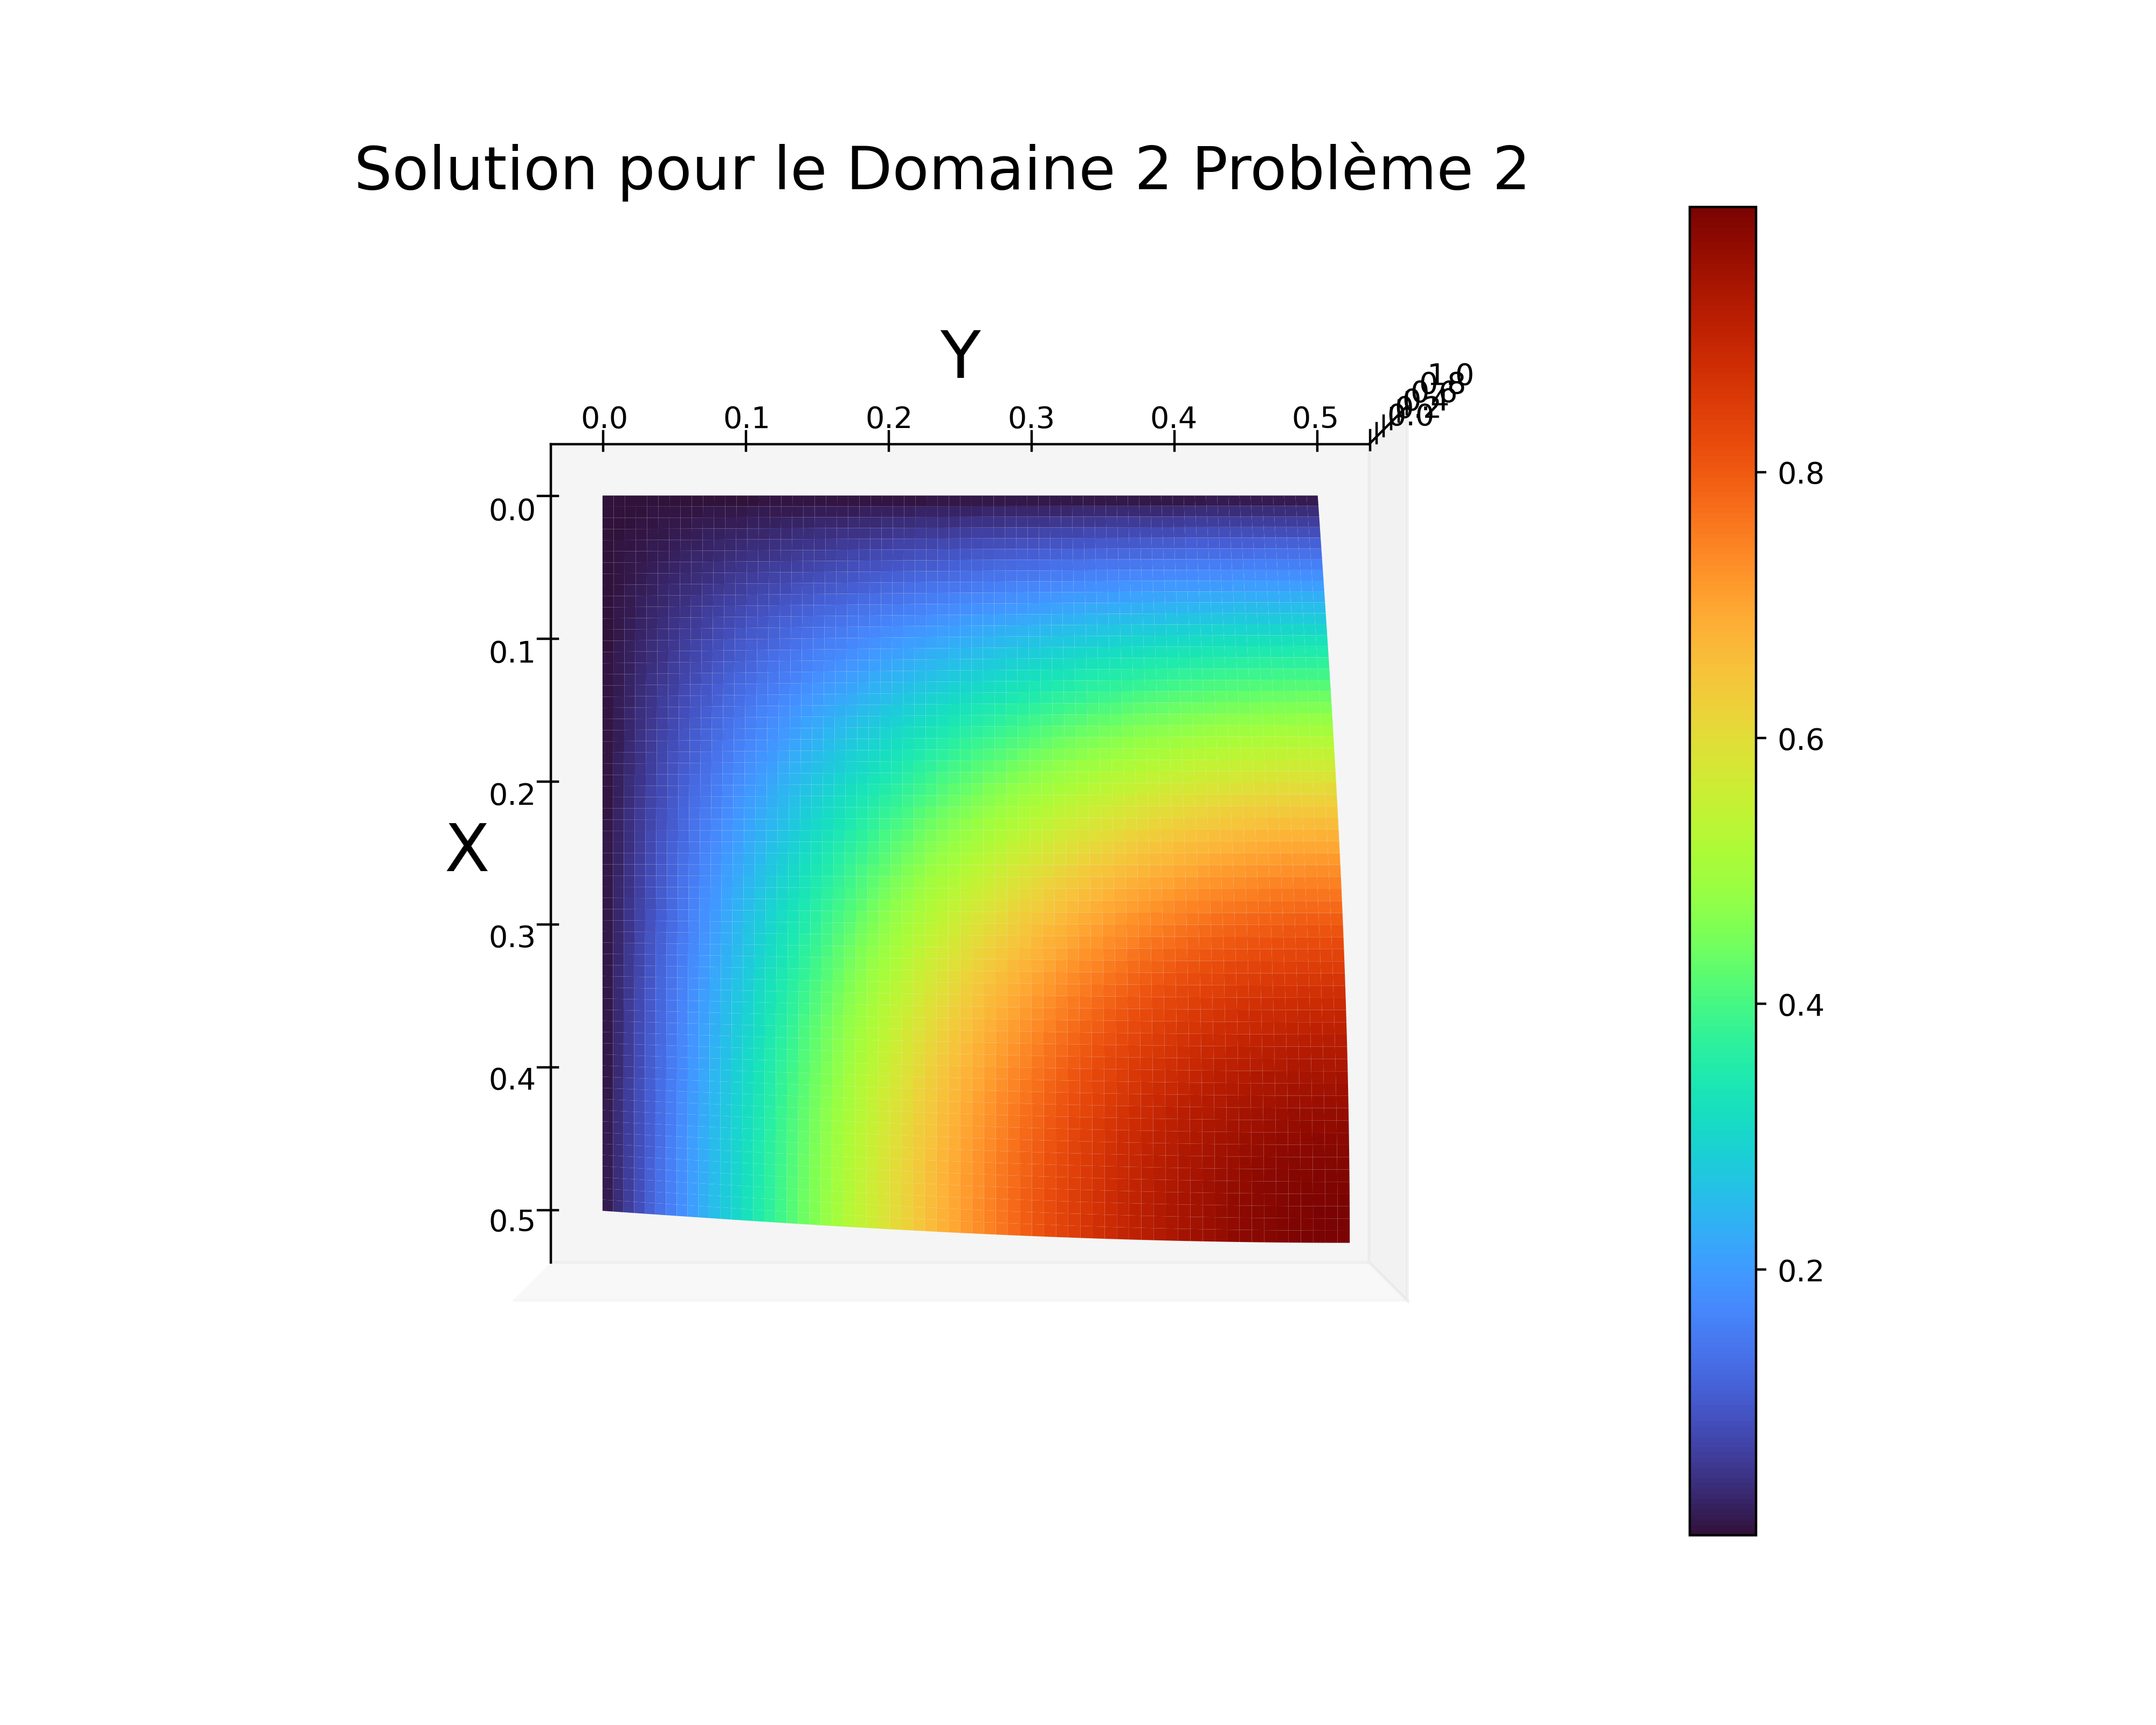
\includegraphics[height=9cm]{../Images/Figures_Calculees/sol3DVH22.png}
    \end{subfigure}
    \caption{Solution calculée vue sous différents angles Domaine 2 Problème 2 }
\end{figure}
\newpage

%%%%%%%%%%%%%%%%%%%%%%%%%%%%%%%%%
\subsection{Problème 3}
%%%%%%%%%%%%%%%%%%%%%%%%%%%%%%%%%
Pour la solution $u=\cos(\pi x)\cos(\pi y)$ :\\
\begin{align*}
    \nabla u(x,y) = \Big( -\pi\sin(\pi x)\cos(\pi y) , -\pi\cos(\pi x)\sin(\pi y) \Big)^T
\end{align*}
On peut donc calculer $f_N$ :
\begin{align*}
    f_N = \left\{
    \begin{array}{ll}
        -\pi\sin(\pi x)\cos(\pi y)  \quad &\text{ sur $\Gamma_1$}\\
        -\pi\cos(\pi x)\sin(\pi y)\quad &\text{ sur $\Gamma_2$}\\
    \end{array}
    \right.
\end{align*}
Ici encore on a toujours la définition des autres fonctions :
\begin{align*}
    &a_{\alpha\beta} = \delta_{\alpha\beta}\\
    &a_{00} = 1\\
    &b_N = 0\\
    & u_D = \cos(\pi x) \cos(\pi y)\\
    & f_\Omega =(1+2\pi^2)\cos(\pi x)\cos(\pi y)
\end{align*}

On peut maintenant exécuter notre programme pour chaque maillage.
Dans un premier temps on utilise des maillages constitués de triangles, on obtient la courbe suivante :

\begin{center}
    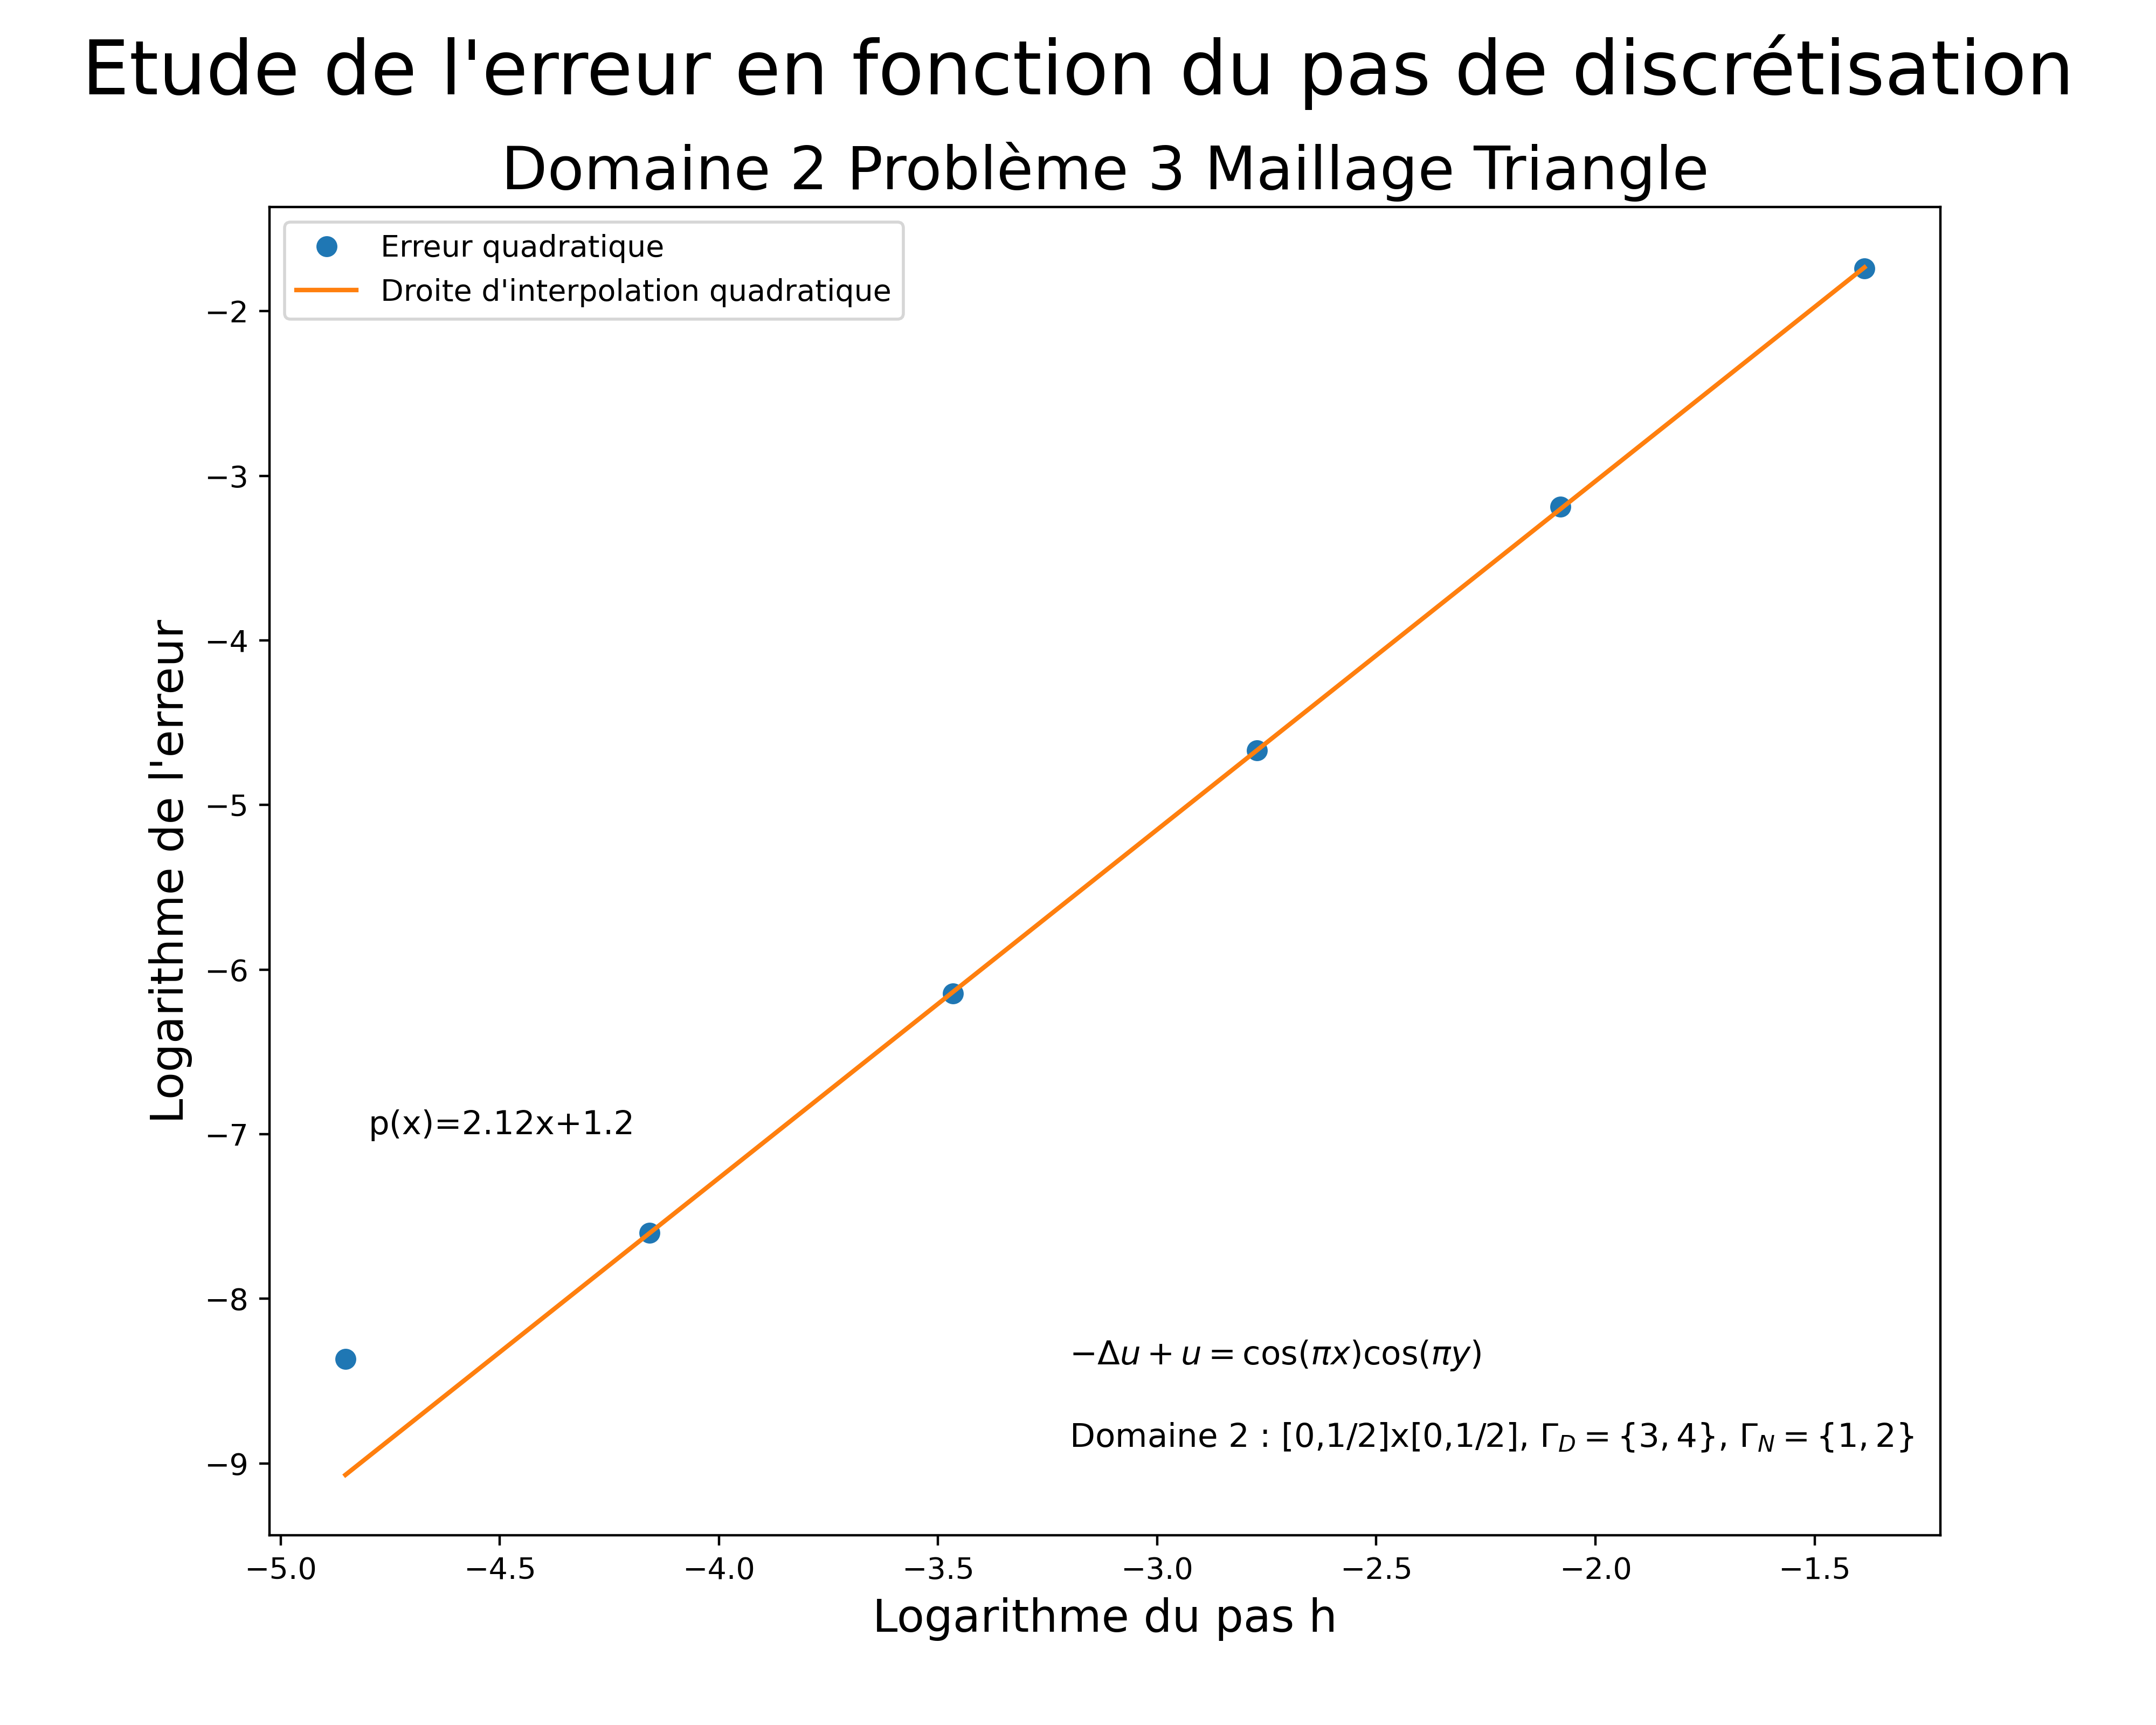
\includegraphics[height=9cm]{../Images/Courbes_Erreurs/D2P3T.png}
\end{center}

Dans un second temps, pour le même problème on utilise un maillage de quadrangle, on obtient alors la courbe suivante :
\begin{center}
    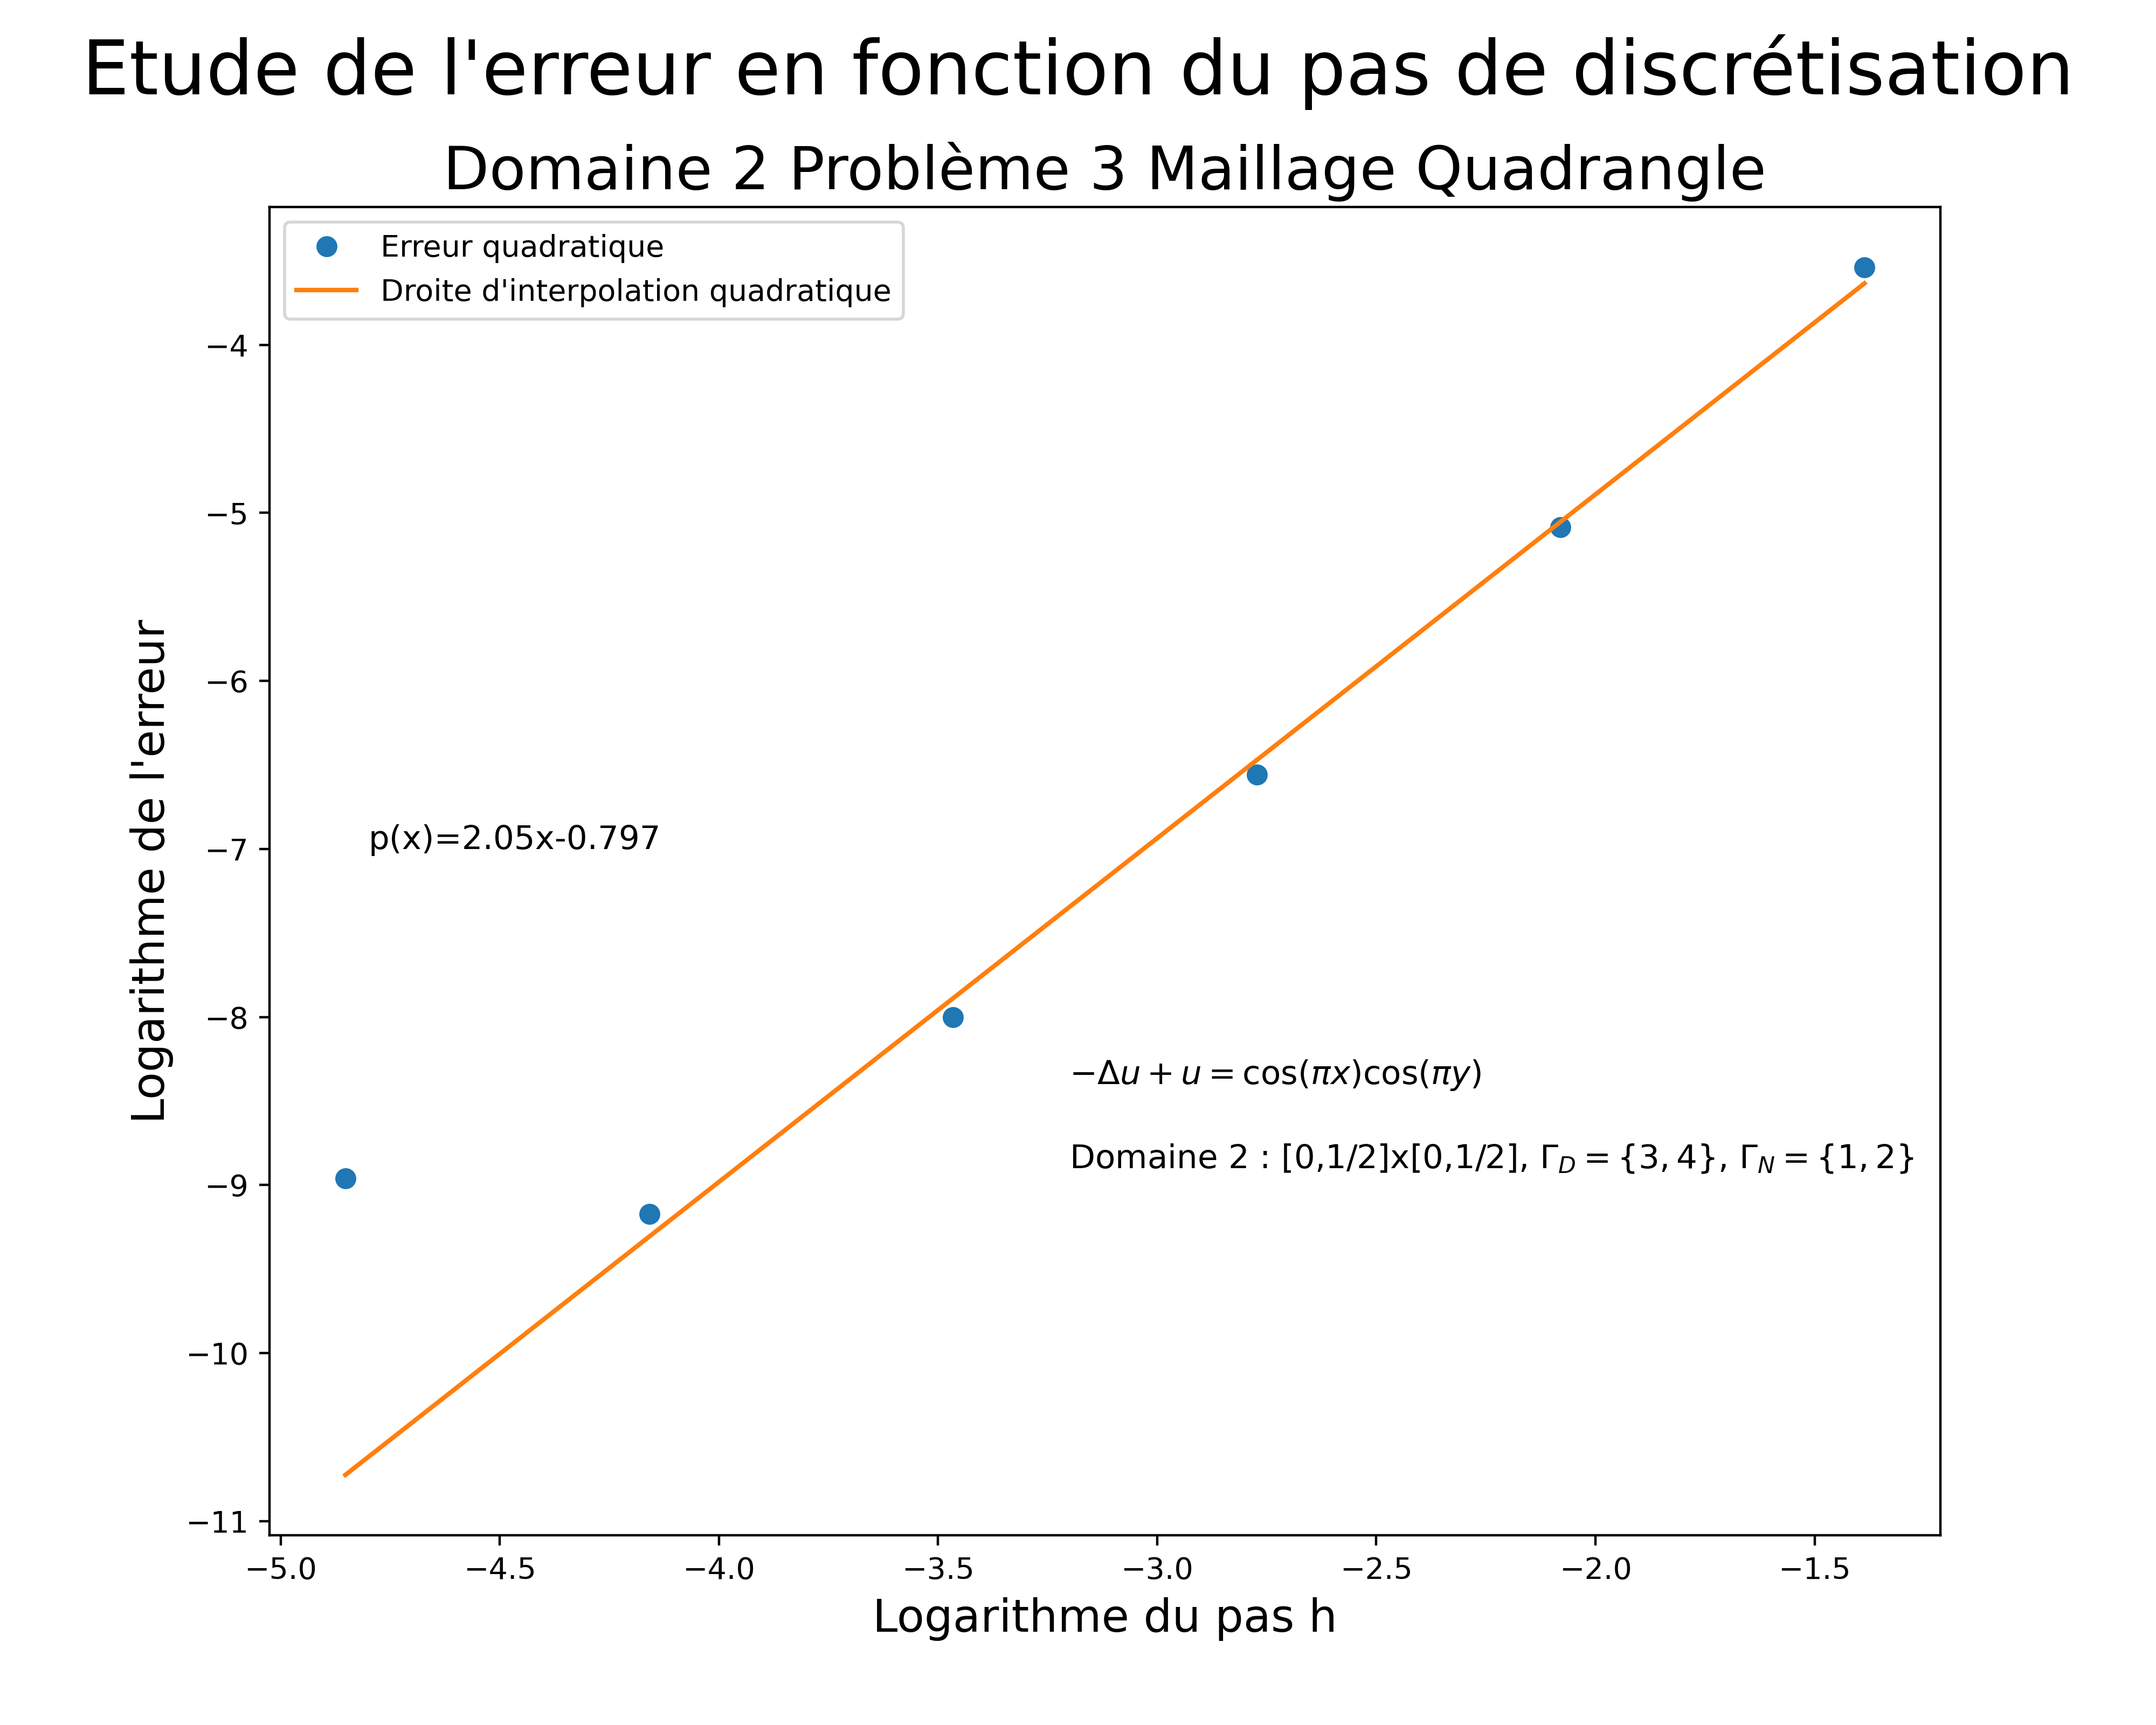
\includegraphics[height=9cm]{../Images/Courbes_Erreurs/D2P3Q.png}
\end{center}

On peut maintenant afficher la solution calculée en 3D pour visualiser la solution.
\begin{figure}[!h]
    \centering
    \begin{subfigure}{0.48\textwidth}
    	\centering
        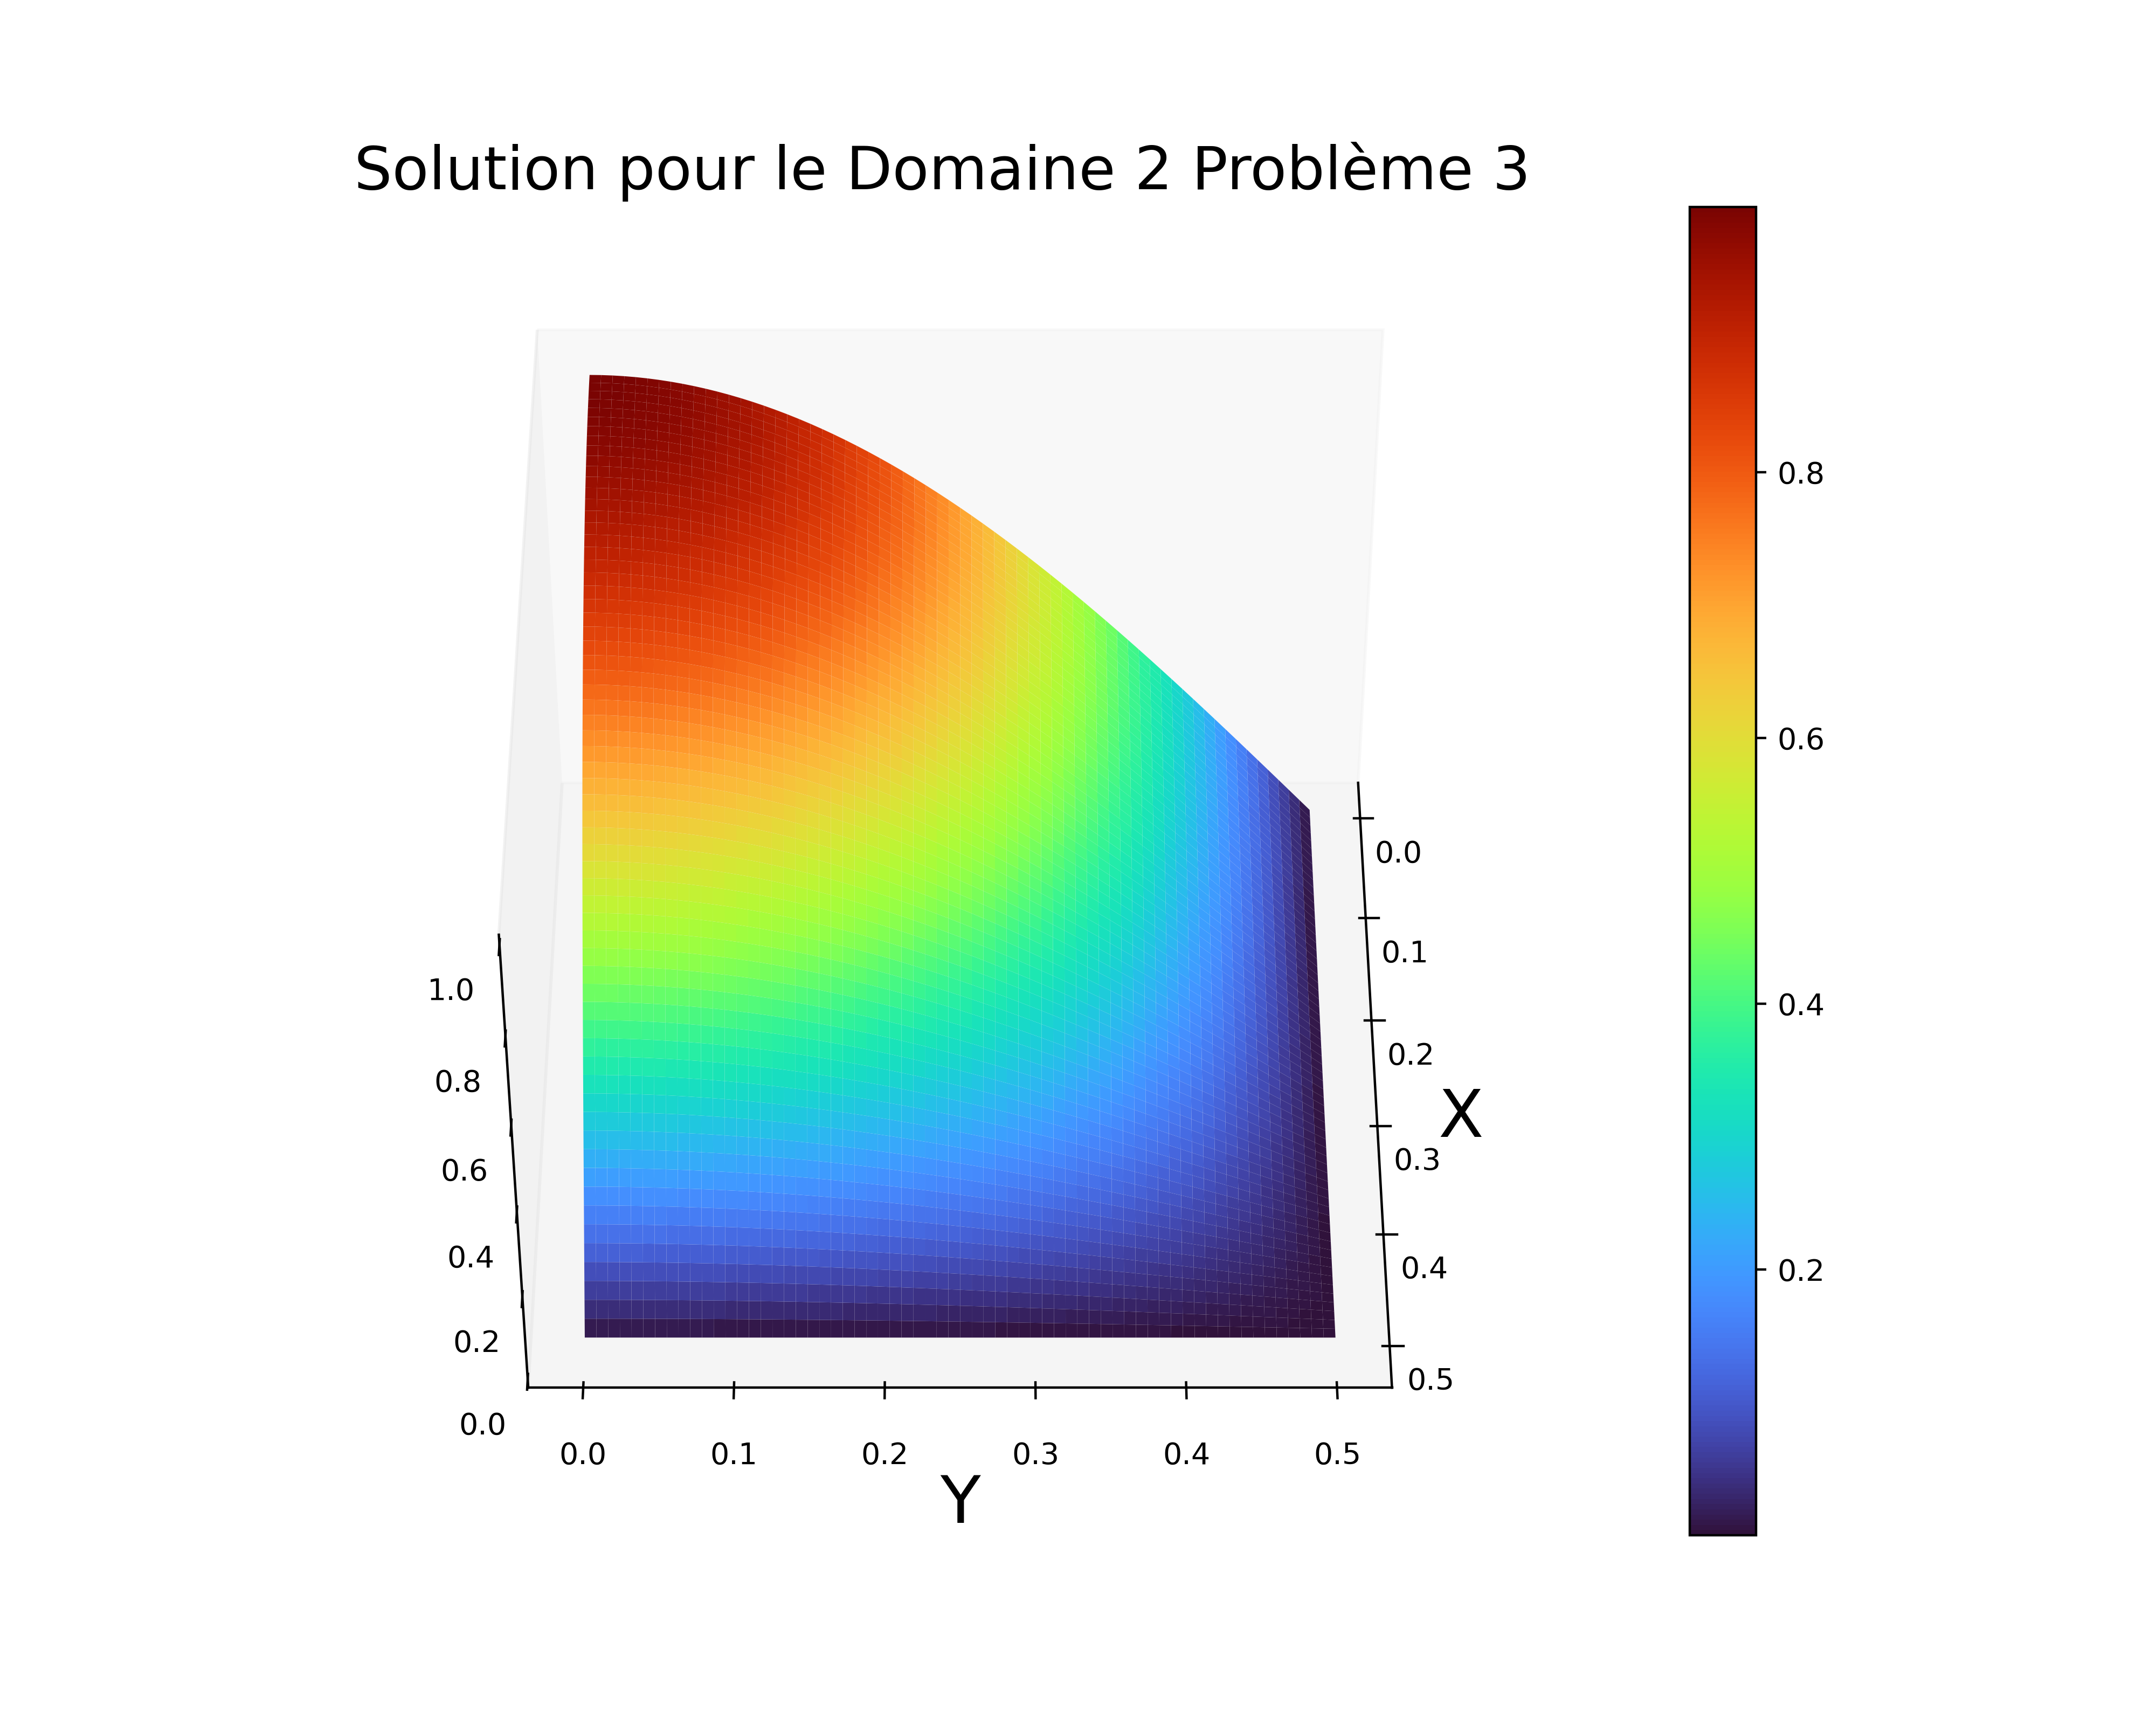
\includegraphics[height=9cm]{../Images/Figures_Calculees/sol3D23.png}
    \end{subfigure}
    \begin{subfigure}{0.48\textwidth}
    \centering
        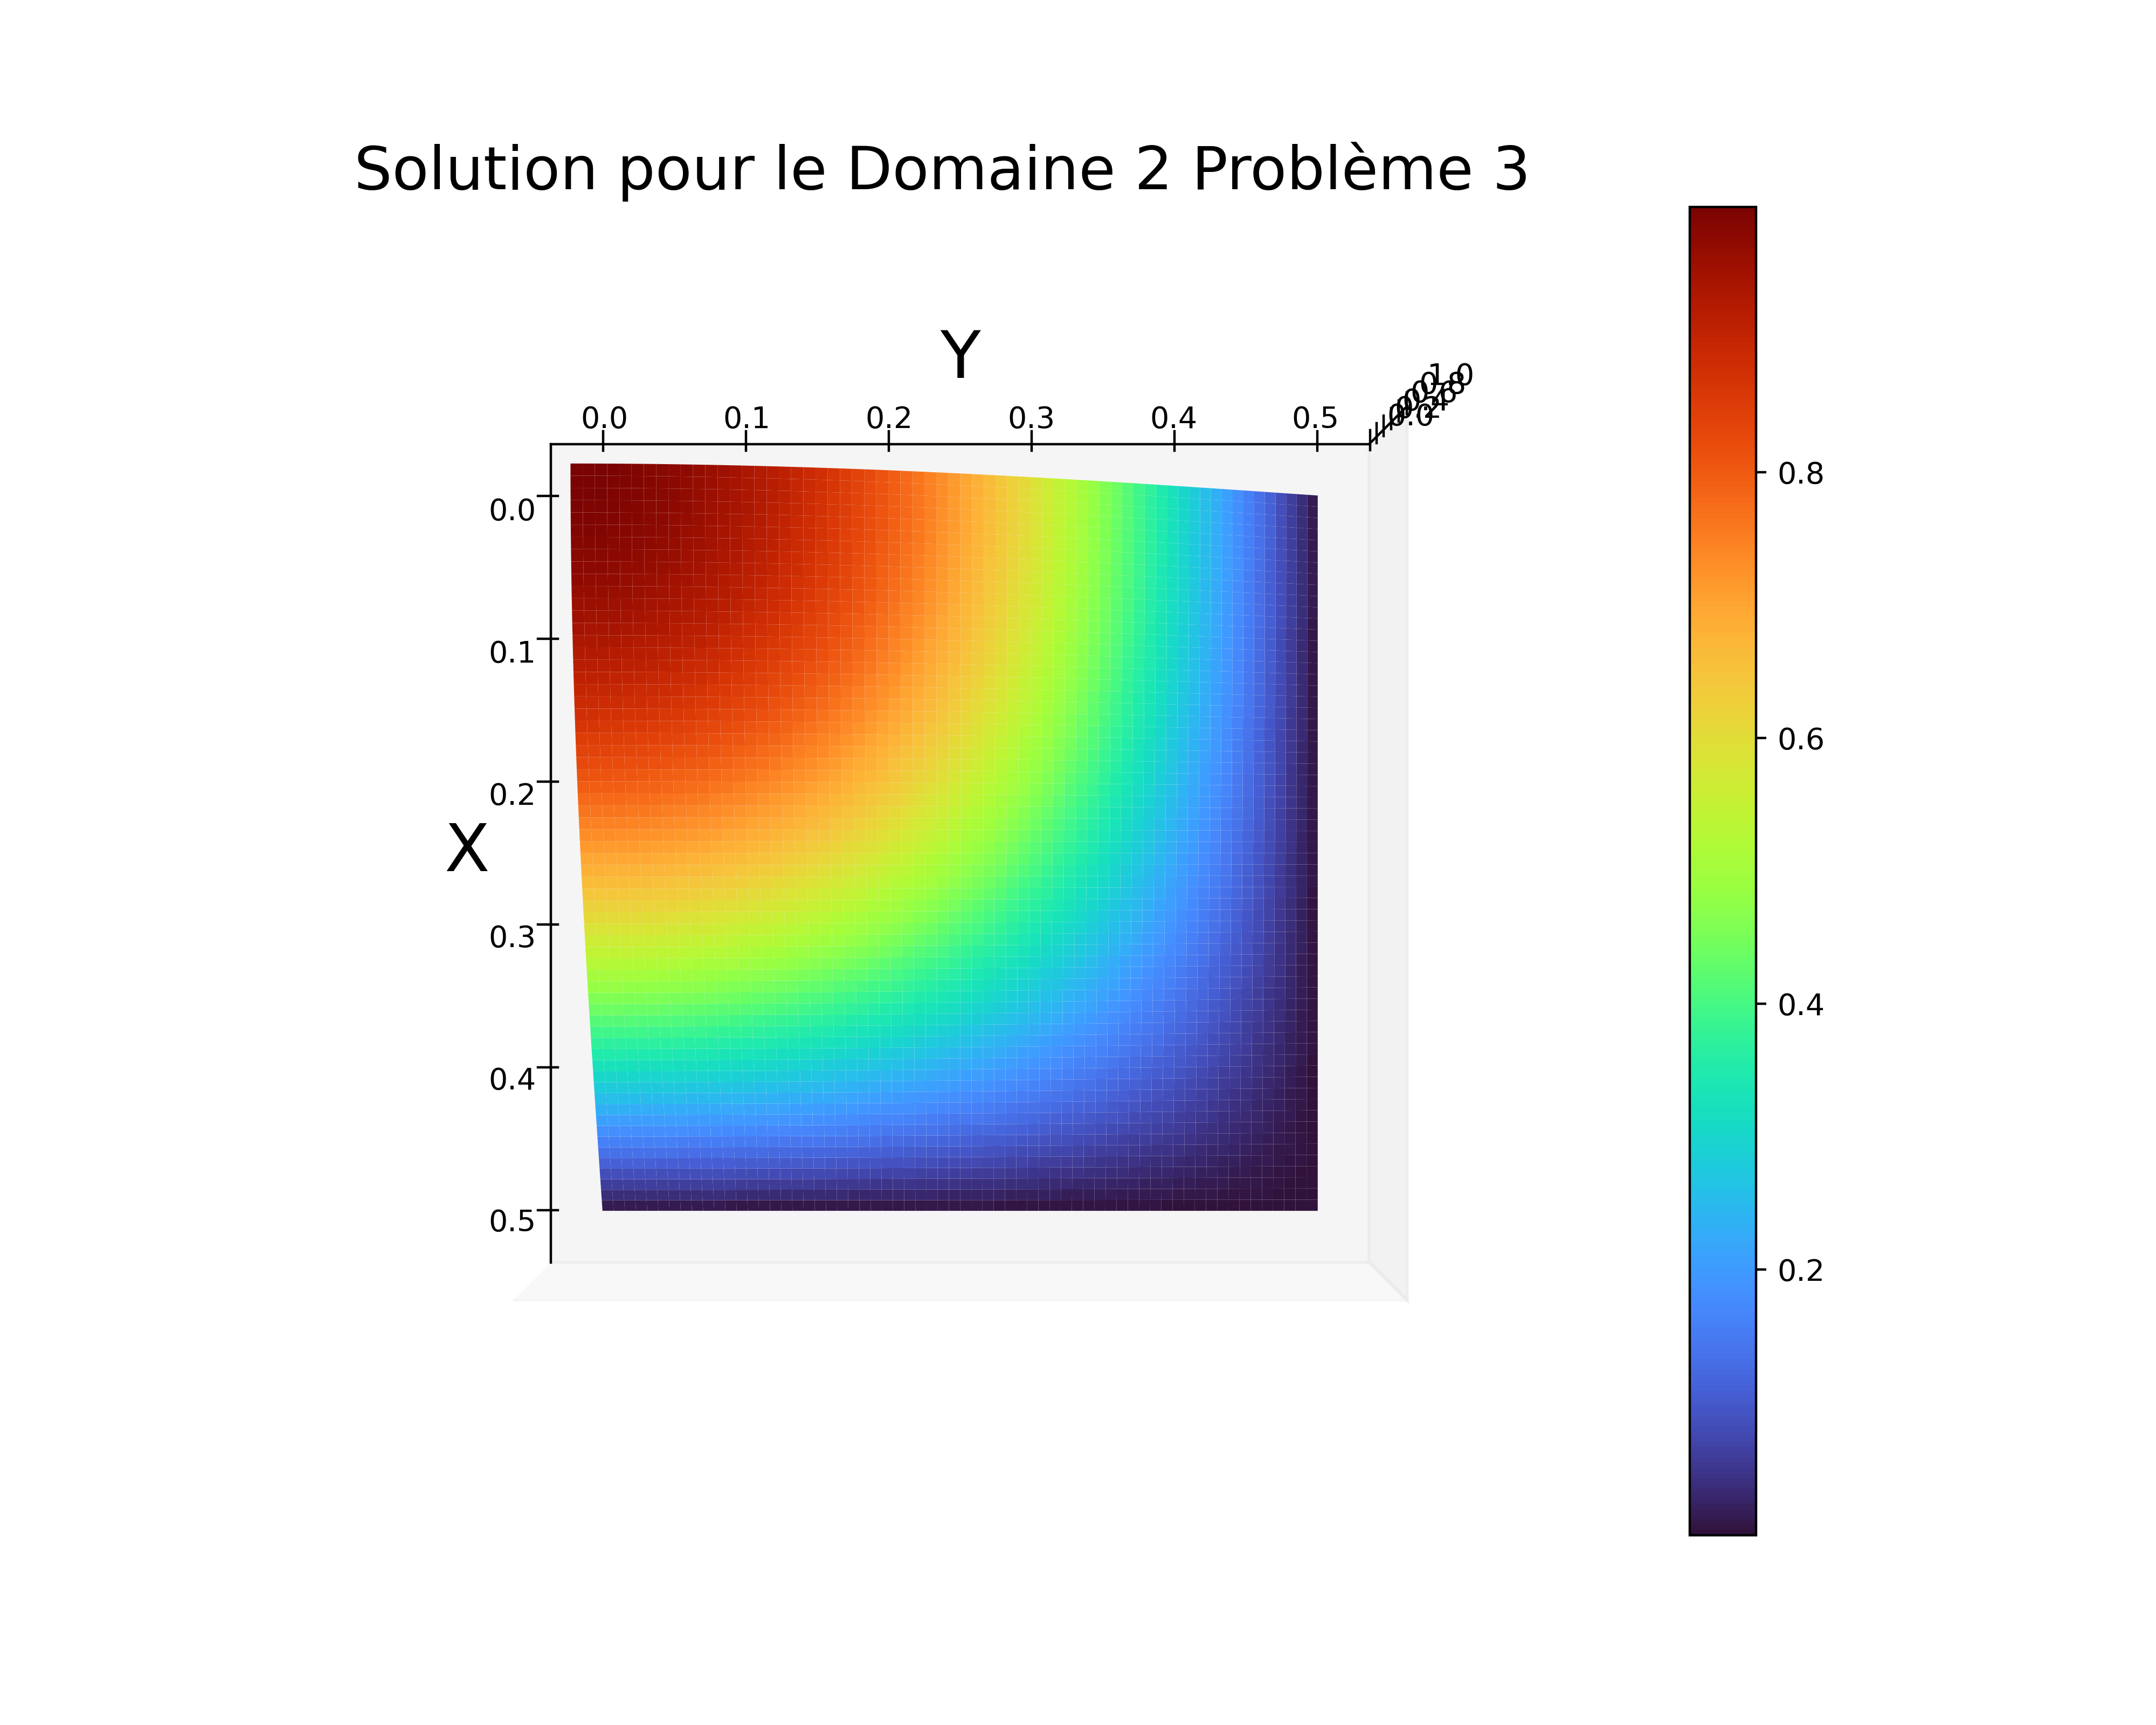
\includegraphics[height=9cm]{../Images/Figures_Calculees/sol3DVH23.png}
    \end{subfigure}
    \caption{Solution calculée vue sous différents angles Domaine 2 Problème 3 }
\end{figure}
\newpage 

\section{Quelques commentaires et analyses}

On peut déjà constater que d'une manière générale, le code pour un maillage de type quadrangle est plus précis que pour un maillage de type triangle. En effet cela peut être expliqué par le fait que le schéma de quadrature est d'ordre 3 pour le quadrangle et d'ordre 2 pour le triangle (ordre 3 aussi pour le segment).\\
Globalement on observe un ordre 2 que ce soit pour un maillage de type triangle ou quadrangle. Dans certain cas, on est quand même assez en dessous de 2 (Problème 1 et 2 du Domaine 2 \ref{D2P1} \ref{D2P2}).\\\\
Par ailleurs, on peut aussi remarquer que sur le domaine 2, on voit qu'un point remonte lorsque le maillage devient de plus en plus petit, on interpole donc que sur les points précédents et on ne prend pas encore compte ce dernier afin d'avoir une interpolation correct.\\
Cela peut être expliqué par le fait que le maillage devient tellement précis que l'erreur d'arrondi devient plus grande que l'erreur du à l'approximation du modèle. Afin d'affiner le calcul il conviendrait de passer à des nombres en double précision, on travaille ici en simple précision. La rigueur et la justesse des calculs pourrait être également revu.\\
On pourrait également utiliser des éléments de référence d'ordre supérieur comme les triangles ou quadrangle d'ordre 2.\\\\
Le code peut être encore amélioré dans sa rapidité sa justesse et optimisation mais également par la prise en compte de maillage 3D, à voir peut-être l'année prochaine.\\\\\\\\\\\\\\\\\\\\\\\\
\textbf{Fin de compte rendu.\\Matthieu Petit / Alexandre Prampart}


\end{document}
